%%%%%%%%%%%%%%%%%%%%%%%%%%%%%%%%

\documentclass[11pt,a4paper]{article}
\usepackage{times}
\usepackage[utf8]{inputenc}
\usepackage[croatian]{babel}
\usepackage[T1]{fontenc} % Latin Modern

%%%%%%%%%%%%%%%%%%%%%%%%%%%%%%%%


%%%%%%%%%%%%%%%%%%%%%%%%%%%%%%%%
%%%%%%%%  MATEMATICKI PAKETI %%%%%%%%%%%
%%%%%%%%%%%%%%%%%%%%%%%%%%%%%%%%

\usepackage{amsmath}
\usepackage{amsfonts}
\usepackage{amssymb}
\usepackage{esvect}
\usepackage{bm}

%%%%%%%%%%%%%%%%%%%%%%%%%%%%%%%%

%%%%%%%%%%%%%%%%%%%%%%%%%%%%%%%%
%%%%%%%%%% PAKETI ZA SLIKE  %%%%%%%%%%%%
%%%%%%%%%%%%%%%%%%%%%%%%%%%%%%%%

\usepackage{graphicx}
\usepackage{float}
\usepackage[hidelinks]{hyperref}
\usepackage{caption}
\usepackage{subcaption}
\usepackage{booktabs}

%%%%%%%%%%%%%%%%%%%%%%%%%%%%%%%%

%%%%%%%%%%%%%%%%%%%%%%%%%%%%%%%%
%%%%%%%%%    PRORED 1.5   %%%%%%%%%%%%%%
%%%%%%%%%%%%%%%%%%%%%%%%%%%%%%%%

\renewcommand{\baselinestretch}{1.5}

%%%%%%%%%%%%%%%%%%%%%%%%%%%%%%%%


%%%%%%%%%%%%%%%%%%%%%%%%%%%%%%%%
%%%%%%%%%% TABLICA - ANTUN %%%%%%%%%%%%
%%%%%%%%%%%%%%%%%%%%%%%%%%%%%%%%

\usepackage{array}
\usepackage{multirow}
\newcolumntype{C}[1]{>{\centering\let\newline\\\arraybackslash\hspace{0pt}}m{#1}}
\newcolumntype{L}[1]{>{\raggedright\let\newline\\\arraybackslash\hspace{0pt}}m{#1}}
\newcolumntype{R}[1]{>{\raggedleft\let\newline\\\arraybackslash\hspace{0pt}}m{#1}}
\usepackage{ctable}

%%%%%%%%%%%%%%%%%%%%%%%%%%%%%%%%

%%%%%%%%%%%%%%%%%%%%%%%%%%%%%%%%
%%%%%%%%%% TABLICA - MARTINA %%%%%%%%%%%
%%%%%%%%%%%%%%%%%%%%%%%%%%%%%%%%

\makeatletter
\renewcommand*\env@matrix[1][\arraystretch]{%
  \edef\arraystretch{#1}%
  \hskip -\arraycolsep
  \let\@ifnextchar\new@ifnextchar
  \array{*\c@MaxMatrixCols c}}
\makeatother



%%%% LATEX KOD ZA KORISTENJE TABLICE %%%%
%%% PRIMJER %%%

%\setlength\extrarowheight{1pt}
%\begin{table}[h]
%\centering
%\caption{Tablica s prikazom }
%\label{prva}
%\begin{tabular}{|l|c|}
%\hline
%\textbf{txt} &  \\ \hline 
%txt & txt    \\ 
%txt & txt   \\ \hline
%txt & txt    \\ \hline
%\end{tabular}
%\end{table}

%%%%%%%%%%%%%%%%%%%%%%%%%%%%%%%%


%%%%%%%%%%%%%%%%%%%%%%%%%%%%%%%%
%%%%%%% DIO ZA UNOS ISJECAKA KODA %%%%%%%%
%%%%%%%%%%%%%%%%%%%%%%%%%%%%%%%%

\usepackage{listings}
\usepackage{color}
 
\definecolor{codegreen}{rgb}{0,0.6,0}
\definecolor{codegray}{rgb}{0.5,0.5,0.5}
\definecolor{codepurple}{rgb}{0.58,0,0.82}
 
\lstdefinestyle{mystyle}{   
    commentstyle=\color{codegreen},
    keywordstyle=\color{blue},
    numberstyle=\tiny\color{codegray},
    stringstyle=\color{codepurple},
    basicstyle=\footnotesize,
    breakatwhitespace=false,         
    breaklines=true,                 
    captionpos=b,                    
    keepspaces=true,                 
    numbers=left,                    
    numbersep=5pt,                  
    showspaces=false,                
    showstringspaces=false,
    showtabs=false,                  
    tabsize=1
}
 
\lstset{style=mystyle}

%\lstinputlisting[language=Matlab, firstline=1, lastline=4, numbers=left, frame=single, label={lst:prvi}, caption={Diskretizacija sustava korištenjem Matlaba}, captionpos=b]{peti.m} 

%%%%%%%%%%%%%%%%%%%%%%%%%%%%%%%%


%----------------------------
% za uredjenje stranice
\usepackage[left=2.5cm,right=2.5cm,top=2.5cm,bottom=2.5cm]{geometry}
\usepackage{fancyhdr}
\pagestyle{fancy} 
\lhead{\leftmark}
\rhead{\rightmark}
\usepackage{titlesec} %za točku iza broja sectiona
\titleformat{\section}{\huge\bfseries}{\thetitle.\quad}{0em}{}
\titleformat{\subsection}{\LARGE\bfseries}{\thetitle.\quad}{0em}{}
\titleformat{\subsubsection}{\Large\bfseries}{\thetitle.\quad}{0em}{}
\titleformat{\paragraph}
{\normalfont\large\bfseries}{\thetitle.\quad}{1em}{}
\titlespacing*{\paragraph}
{0pt}{3.25ex plus 1ex minus .2ex}{1.5ex plus .2ex}
\setcounter{secnumdepth}{5}

\usepackage{indentfirst} %uvlacenje prvog paragrafa
% primjer pozivanja sectiona
% \section*{UVOD} \pdfbookmark{UVOD}{section:UVOD}

\usepackage{tocloft}
\usepackage{import}
\usepackage{standalone}

\graphicspath{{Uvod/figures/}, {CAD/}, {Exp/}, {Hardware/}, {Software/}, {Identifikacija/figures/}, {Koncept/figures/}, {Model/figures/}, {Software/Slike/}, {Hardware/figures/},{CAD/figures/}, {Uvod/figures/},{Exp/figures/}, {Kontrola/figures/}}

\hypersetup{
  colorlinks   = true, %Colours links instead of ugly boxes
  urlcolor     = black, %Colour for external hyperlinks
  linkcolor    = black, %Colour of internal links
  citecolor   = blue %Colour of citations
}

\usepackage{subcaption}
\usepackage{lscape}
\begin{document}

\begin{titlepage}

%%%%%%%%%%%%%%%%%%%%%%%%%%%%%%%%
%%%%%%% NASLOVNA STRANICA %%%%%%%%%%%%
%%%%%%%%%%%%%%%%%%%%%%%%%%%%%%%%

\center

\textsc{\huge Sveučilište u Zagrebu} \\
\textsc{\huge Fakultet Elektrotehnike i Računarstva}

\vspace*{\fill}
\emph{\large Matija Bedeković, Bruno Marić, Martina Tomić}\\
\vspace{0.5cm}
\begin{Huge}
	Dizajn i razvoj male multirotorske letjelice s upravljanjem zasnovanim na pomičnim masama
\end{Huge}
\vspace*{\fill}

Zagreb, \the\year

%%%%%%%%%%%%%%%%%%%%%%%%%%%%%%%%

%%%%%%%%%%%%%%%%%%%%%%%%%%%%%%%%
%%%%%% DRUGA STRANICA - TRAZENI OPIS %%%%%%%
%%%%%%%%%%%%%%%%%%%%%%%%%%%%%%%%

\newpage
\thispagestyle{empty}
\vspace*{\fill}
\begin{large}
	Ovaj rad izrađen je u Laboratoriju za Robotiku i Inteligentne Sustave Upravljanja, na Zavodu za Automatiku i Računalno Inženjerstvo pod vodstvom prof. dr. sc. Stjepana Bogdana i predan je za natječaj za dodjelu Rektorove nagrade u akademskoj godini 2016./2017.
	\end{large}
\vspace*{\fill}
\end{titlepage}

%%%%%%%%%%%%%%%%%%%%%%%%%%%%%%%%

%%%%%%%%%%%%%%%%%%%%%%%%%%%%%%%
%% UBACIVANJE SADRZAJA, POPISA SLIKA I TABLICA %%
%%%%%%%%%%%%%%%%%%%%%%%%%%%%%%%

\renewcommand{\cftsecleader}{\cftdotfill{\cftdotsep}}
\newpage
\tableofcontents
\thispagestyle{empty}
\newpage
\listoffigures
\thispagestyle{empty}
\newpage
\listoftables
\thispagestyle{empty}

%%%%%%%%%%%%%%%%%%%%%%%%%%%%%%%

%%%%%%%%%%%%%%%%%%%%%%%%%%%%%%%
%%%%%%%%TAKSTUALNI DIO RADA %%%%%%%%%%
%%%%%%%%%%%%%%%%%%%%%%%%%%%%%%%


\newpage
%%%%% ODKOMENTIRATI DA UVOD BUDE STRANICA 1 %%%%%%
\setcounter{page}{1}
\section{Uvod}
%%%%%%%%%%%%%%%%%%%%%%%%%%%%%%%%

\documentclass[11pt,a4paper]{article}
\usepackage{times}
\usepackage[utf8]{inputenc}
\usepackage[croatian]{babel}
\usepackage[T1]{fontenc} % Latin Modern

%%%%%%%%%%%%%%%%%%%%%%%%%%%%%%%%


%%%%%%%%%%%%%%%%%%%%%%%%%%%%%%%%
%%%%%%%%  MATEMATICKI PAKETI %%%%%%%%%%%
%%%%%%%%%%%%%%%%%%%%%%%%%%%%%%%%

\usepackage{amsmath}
\usepackage{amsfonts}
\usepackage{amssymb}
\usepackage{esvect}

%%%%%%%%%%%%%%%%%%%%%%%%%%%%%%%%

%%%%%%%%%%%%%%%%%%%%%%%%%%%%%%%%
%%%%%%%%%% PAKETI ZA SLIKE  %%%%%%%%%%%%
%%%%%%%%%%%%%%%%%%%%%%%%%%%%%%%%

\usepackage{graphicx}
\usepackage{float}
\usepackage[hidelinks]{hyperref}
\usepackage{caption}
\usepackage{subcaption}
\usepackage{booktabs}

%%%%%%%%%%%%%%%%%%%%%%%%%%%%%%%%

%%%%%%%%%%%%%%%%%%%%%%%%%%%%%%%%
%%%%%%%%%    PRORED 1.5   %%%%%%%%%%%%%%
%%%%%%%%%%%%%%%%%%%%%%%%%%%%%%%%

\renewcommand{\baselinestretch}{1.5}

%%%%%%%%%%%%%%%%%%%%%%%%%%%%%%%%


%%%%%%%%%%%%%%%%%%%%%%%%%%%%%%%%
%%%%%%%%%% TABLICA - ANTUN %%%%%%%%%%%%
%%%%%%%%%%%%%%%%%%%%%%%%%%%%%%%%

\usepackage{array}
\usepackage{multirow}
\newcolumntype{C}[1]{>{\centering\let\newline\\\arraybackslash\hspace{0pt}}m{#1}}
\newcolumntype{L}[1]{>{\raggedright\let\newline\\\arraybackslash\hspace{0pt}}m{#1}}
\newcolumntype{R}[1]{>{\raggedleft\let\newline\\\arraybackslash\hspace{0pt}}m{#1}}
\usepackage{ctable}

%%%%%%%%%%%%%%%%%%%%%%%%%%%%%%%%

%%%%%%%%%%%%%%%%%%%%%%%%%%%%%%%%
%%%%%%%%%% TABLICA - MARTINA %%%%%%%%%%%
%%%%%%%%%%%%%%%%%%%%%%%%%%%%%%%%

\makeatletter
\renewcommand*\env@matrix[1][\arraystretch]{%
  \edef\arraystretch{#1}%
  \hskip -\arraycolsep
  \let\@ifnextchar\new@ifnextchar
  \array{*\c@MaxMatrixCols c}}
\makeatother



%%%% LATEX KOD ZA KORISTENJE TABLICE %%%%
%%% PRIMJER %%%

%\setlength\extrarowheight{1pt}
%\begin{table}[h]
%\centering
%\caption{Tablica s prikazom }
%\label{prva}
%\begin{tabular}{|l|c|}
%\hline
%\textbf{txt} &  \\ \hline 
%txt & txt    \\ 
%txt & txt   \\ \hline
%txt & txt    \\ \hline
%\end{tabular}
%\end{table}

%%%%%%%%%%%%%%%%%%%%%%%%%%%%%%%%


%%%%%%%%%%%%%%%%%%%%%%%%%%%%%%%%
%%%%%%% DIO ZA UNOS ISJECAKA KODA %%%%%%%%
%%%%%%%%%%%%%%%%%%%%%%%%%%%%%%%%

\usepackage{listings}
\usepackage{color}
 
\definecolor{codegreen}{rgb}{0,0.6,0}
\definecolor{codegray}{rgb}{0.5,0.5,0.5}
\definecolor{codepurple}{rgb}{0.58,0,0.82}
 
\lstdefinestyle{mystyle}{   
    commentstyle=\color{codegreen},
    keywordstyle=\color{blue},
    numberstyle=\tiny\color{codegray},
    stringstyle=\color{codepurple},
    basicstyle=\footnotesize,
    breakatwhitespace=false,         
    breaklines=true,                 
    captionpos=b,                    
    keepspaces=true,                 
    numbers=left,                    
    numbersep=5pt,                  
    showspaces=false,                
    showstringspaces=false,
    showtabs=false,                  
    tabsize=1
}
 
\lstset{style=mystyle}

%\lstinputlisting[language=Matlab, firstline=1, lastline=4, numbers=left, frame=single, label={lst:prvi}, caption={Diskretizacija sustava korištenjem Matlaba}, captionpos=b]{peti.m} 

%%%%%%%%%%%%%%%%%%%%%%%%%%%%%%%%


%----------------------------
% za uredjenje stranice
\usepackage[left=2.5cm,right=2.5cm,top=2.5cm,bottom=2.5cm]{geometry}
\usepackage{fancyhdr}
\pagestyle{fancy} 
\lhead{\leftmark}
\rhead{\rightmark}
\usepackage{titlesec} %za točku iza broja sectiona
\titleformat{\section}{\huge\bfseries}{\thetitle.\quad}{0em}{}
\titleformat{\subsection}{\LARGE\bfseries}{\thetitle.\quad}{0em}{}
\titleformat{\subsubsection}{\Large\bfseries}{\thetitle.\quad}{0em}{}
\titleformat{\paragraph}
{\normalfont\large\bfseries}{\thetitle.\quad}{1em}{}
\titlespacing*{\paragraph}
{0pt}{3.25ex plus 1ex minus .2ex}{1.5ex plus .2ex}
\setcounter{secnumdepth}{5}

\usepackage{indentfirst} %uvlacenje prvog paragrafa
% primjer pozivanja sectiona
% \section*{UVOD} \pdfbookmark{UVOD}{section:UVOD}

\usepackage{tocloft}
\usepackage{import}
\usepackage{standalone}
\graphicspath{{Uvod/}, {Ciljevi/}, {Materijal/}, {Rasprava/}, {Rezultati/}} 

\hypersetup{
  colorlinks   = true, %Colours links instead of ugly boxes
  urlcolor     = black, %Colour for external hyperlinks
  linkcolor    = black, %Colour of internal links
  citecolor   = blue %Colour of citations
}

\usepackage{subcaption}
\usepackage{lscape}
\begin{document}


UVOD

whriwurhwiehrw

\end{document}

\newpage
\section{Opis koncepta} 
%%%%%%%%%%%%%%%%%%%%%%%%%%%%%%%%

\documentclass[11pt,a4paper]{article}
\usepackage{times}
\usepackage[utf8]{inputenc}
\usepackage[croatian]{babel}
\usepackage[T1]{fontenc} % Latin Modern

%%%%%%%%%%%%%%%%%%%%%%%%%%%%%%%%


%%%%%%%%%%%%%%%%%%%%%%%%%%%%%%%%
%%%%%%%%  MATEMATICKI PAKETI %%%%%%%%%%%
%%%%%%%%%%%%%%%%%%%%%%%%%%%%%%%%

\usepackage{amsmath}
\usepackage{amsfonts}
\usepackage{amssymb}
\usepackage{esvect}

%%%%%%%%%%%%%%%%%%%%%%%%%%%%%%%%

%%%%%%%%%%%%%%%%%%%%%%%%%%%%%%%%
%%%%%%%%%% PAKETI ZA SLIKE  %%%%%%%%%%%%
%%%%%%%%%%%%%%%%%%%%%%%%%%%%%%%%

\usepackage{graphicx}
\usepackage{float}
\usepackage[hidelinks]{hyperref}
\usepackage{caption}
\usepackage{subcaption}
\usepackage{booktabs}

%%%%%%%%%%%%%%%%%%%%%%%%%%%%%%%%

%%%%%%%%%%%%%%%%%%%%%%%%%%%%%%%%
%%%%%%%%%    PRORED 1.5   %%%%%%%%%%%%%%
%%%%%%%%%%%%%%%%%%%%%%%%%%%%%%%%

\renewcommand{\baselinestretch}{1.5}

%%%%%%%%%%%%%%%%%%%%%%%%%%%%%%%%


%%%%%%%%%%%%%%%%%%%%%%%%%%%%%%%%
%%%%%%%%%% TABLICA - ANTUN %%%%%%%%%%%%
%%%%%%%%%%%%%%%%%%%%%%%%%%%%%%%%

\usepackage{array}
\usepackage{multirow}
\newcolumntype{C}[1]{>{\centering\let\newline\\\arraybackslash\hspace{0pt}}m{#1}}
\newcolumntype{L}[1]{>{\raggedright\let\newline\\\arraybackslash\hspace{0pt}}m{#1}}
\newcolumntype{R}[1]{>{\raggedleft\let\newline\\\arraybackslash\hspace{0pt}}m{#1}}
\usepackage{ctable}

%%%%%%%%%%%%%%%%%%%%%%%%%%%%%%%%

%%%%%%%%%%%%%%%%%%%%%%%%%%%%%%%%
%%%%%%%%%% TABLICA - MARTINA %%%%%%%%%%%
%%%%%%%%%%%%%%%%%%%%%%%%%%%%%%%%

\makeatletter
\renewcommand*\env@matrix[1][\arraystretch]{%
  \edef\arraystretch{#1}%
  \hskip -\arraycolsep
  \let\@ifnextchar\new@ifnextchar
  \array{*\c@MaxMatrixCols c}}
\makeatother



%%%% LATEX KOD ZA KORISTENJE TABLICE %%%%
%%% PRIMJER %%%

%\setlength\extrarowheight{1pt}
%\begin{table}[h]
%\centering
%\caption{Tablica s prikazom }
%\label{prva}
%\begin{tabular}{|l|c|}
%\hline
%\textbf{txt} &  \\ \hline 
%txt & txt    \\ 
%txt & txt   \\ \hline
%txt & txt    \\ \hline
%\end{tabular}
%\end{table}

%%%%%%%%%%%%%%%%%%%%%%%%%%%%%%%%


%%%%%%%%%%%%%%%%%%%%%%%%%%%%%%%%
%%%%%%% DIO ZA UNOS ISJECAKA KODA %%%%%%%%
%%%%%%%%%%%%%%%%%%%%%%%%%%%%%%%%

\usepackage{listings}
\usepackage{color}
 
\definecolor{codegreen}{rgb}{0,0.6,0}
\definecolor{codegray}{rgb}{0.5,0.5,0.5}
\definecolor{codepurple}{rgb}{0.58,0,0.82}
 
\lstdefinestyle{mystyle}{   
    commentstyle=\color{codegreen},
    keywordstyle=\color{blue},
    numberstyle=\tiny\color{codegray},
    stringstyle=\color{codepurple},
    basicstyle=\footnotesize,
    breakatwhitespace=false,         
    breaklines=true,                 
    captionpos=b,                    
    keepspaces=true,                 
    numbers=left,                    
    numbersep=5pt,                  
    showspaces=false,                
    showstringspaces=false,
    showtabs=false,                  
    tabsize=1
}
 
\lstset{style=mystyle}

%\lstinputlisting[language=Matlab, firstline=1, lastline=4, numbers=left, frame=single, label={lst:prvi}, caption={Diskretizacija sustava korištenjem Matlaba}, captionpos=b]{peti.m} 

%%%%%%%%%%%%%%%%%%%%%%%%%%%%%%%%


%----------------------------
% za uredjenje stranice
\usepackage[left=2.5cm,right=2.5cm,top=2.5cm,bottom=2.5cm]{geometry}
\usepackage{fancyhdr}
\pagestyle{fancy} 
\lhead{\leftmark}
\rhead{\rightmark}
\usepackage{titlesec} %za točku iza broja sectiona
\titleformat{\section}{\huge\bfseries}{\thetitle.\quad}{0em}{}
\titleformat{\subsection}{\LARGE\bfseries}{\thetitle.\quad}{0em}{}
\titleformat{\subsubsection}{\Large\bfseries}{\thetitle.\quad}{0em}{}
\titleformat{\paragraph}
{\normalfont\large\bfseries}{\thetitle.\quad}{1em}{}
\titlespacing*{\paragraph}
{0pt}{3.25ex plus 1ex minus .2ex}{1.5ex plus .2ex}
\setcounter{secnumdepth}{5}

\usepackage{indentfirst} %uvlacenje prvog paragrafa
% primjer pozivanja sectiona
% \section*{UVOD} \pdfbookmark{UVOD}{section:UVOD}

\usepackage{tocloft}
\usepackage{import}
\usepackage{standalone}
\graphicspath{{Koncept/figures/}} 

\hypersetup{
  colorlinks   = true, %Colours links instead of ugly boxes
  urlcolor     = black, %Colour for external hyperlinks
  linkcolor    = black, %Colour of internal links
  citecolor   = blue %Colour of citations
}

\usepackage{subcaption}
\usepackage{lscape}
\begin{document}

Promjena centra mase letjelice postiže se promjenom pozicije pomičnih masa smještenih na krakove letjelice. Ta promjena uzrokuje nastanak momenata kuteva  valjanja (\textit{roll}) i poniranja (\textit{pitch}), što zauzvrat služi za kontrolu pozicije letjelice. Grafički prikaz uzroka i posljedice ovog koncepta upravljanja prikazan je Slikom \ref{fig:kontrol}. Kako bi upravljanje kutevima valjanja i poniranja bilo raspregnuto, multirotorska letjelica mora biti konstruirana u standardnoj \textit{plus konfiguraciji} \cite{haus1}.

\bigskip

\begin{figure}[H]
	\centering
	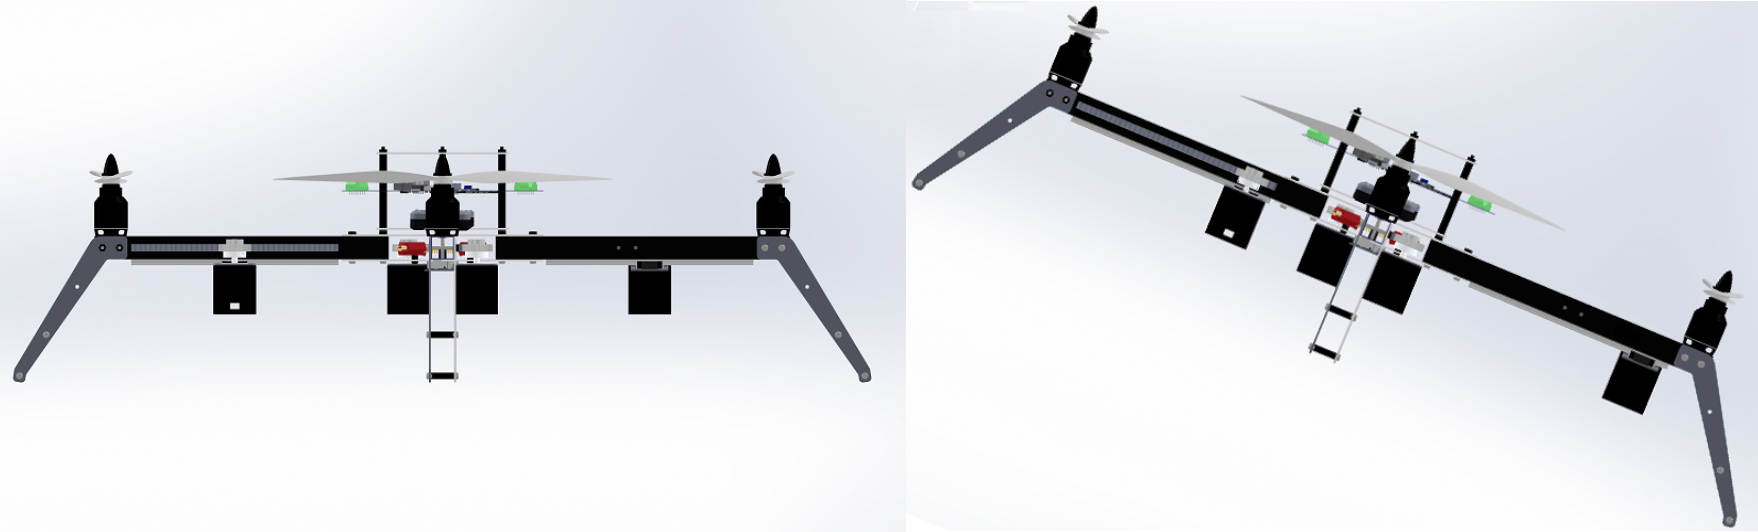
\includegraphics[width=\textwidth]{roll_koncept}
	\caption{Utjecaj pomaka pokretne mase na položaj letjelice}
	\label{fig:kontrol}
\end{figure}


Bitno je naglasiti kako se za upravljanje visine letjelice te kuta njezinog zakreta i dalje koristi klasična metoda upravljanja, ona zasnovana na promjeni brzine vrtnje propelera. Dinamika letjelice po visini i zakretanju je sporija od dinamike valjanja i poniranja te se očekuje kako će benzinski motori moći upravljati s tim stupnjevima slobode. U nastavku ovog rada glavni će fokus biti na novom konceptu upravljanja kutevima poniranja i valjanja multirotorske letjelice. 


\end{document}






\newpage
\section{Matematički model}
%%%%%%%%%%%%%%%%%%%%%%%%%%%%%%%%

\documentclass[11pt,a4paper]{article}
\usepackage{times}
\usepackage[utf8]{inputenc}
\usepackage[croatian]{babel}
\usepackage[T1]{fontenc} % Latin Modern

%%%%%%%%%%%%%%%%%%%%%%%%%%%%%%%%


%%%%%%%%%%%%%%%%%%%%%%%%%%%%%%%%
%%%%%%%%  MATEMATICKI PAKETI %%%%%%%%%%%
%%%%%%%%%%%%%%%%%%%%%%%%%%%%%%%%

\usepackage{amsmath}
\usepackage{amsfonts}
\usepackage{amssymb}
\usepackage{esvect}
\usepackage{bm}

%%%%%%%%%%%%%%%%%%%%%%%%%%%%%%%%

%%%%%%%%%%%%%%%%%%%%%%%%%%%%%%%%
%%%%%%%%%% PAKETI ZA SLIKE  %%%%%%%%%%%%
%%%%%%%%%%%%%%%%%%%%%%%%%%%%%%%%

\usepackage{graphicx}
\usepackage{float}
\usepackage[hidelinks]{hyperref}
\usepackage{caption}
\usepackage{subcaption}
\usepackage{booktabs}

%%%%%%%%%%%%%%%%%%%%%%%%%%%%%%%%

%%%%%%%%%%%%%%%%%%%%%%%%%%%%%%%%
%%%%%%%%%    PRORED 1.5   %%%%%%%%%%%%%%
%%%%%%%%%%%%%%%%%%%%%%%%%%%%%%%%

\renewcommand{\baselinestretch}{1.5}

%%%%%%%%%%%%%%%%%%%%%%%%%%%%%%%%


%%%%%%%%%%%%%%%%%%%%%%%%%%%%%%%%
%%%%%%%%%% TABLICA - ANTUN %%%%%%%%%%%%
%%%%%%%%%%%%%%%%%%%%%%%%%%%%%%%%

\usepackage{array}
\usepackage{multirow}
\newcolumntype{C}[1]{>{\centering\let\newline\\\arraybackslash\hspace{0pt}}m{#1}}
\newcolumntype{L}[1]{>{\raggedright\let\newline\\\arraybackslash\hspace{0pt}}m{#1}}
\newcolumntype{R}[1]{>{\raggedleft\let\newline\\\arraybackslash\hspace{0pt}}m{#1}}
\usepackage{ctable}

%%%%%%%%%%%%%%%%%%%%%%%%%%%%%%%%

%%%%%%%%%%%%%%%%%%%%%%%%%%%%%%%%
%%%%%%%%%% TABLICA - MARTINA %%%%%%%%%%%
%%%%%%%%%%%%%%%%%%%%%%%%%%%%%%%%

\makeatletter
\renewcommand*\env@matrix[1][\arraystretch]{%
  \edef\arraystretch{#1}%
  \hskip -\arraycolsep
  \let\@ifnextchar\new@ifnextchar
  \array{*\c@MaxMatrixCols c}}
\makeatother



%%%% LATEX KOD ZA KORISTENJE TABLICE %%%%
%%% PRIMJER %%%

%\setlength\extrarowheight{1pt}
%\begin{table}[h]
%\centering
%\caption{Tablica s prikazom }
%\label{prva}
%\begin{tabular}{|l|c|}
%\hline
%\textbf{txt} &  \\ \hline 
%txt & txt    \\ 
%txt & txt   \\ \hline
%txt & txt    \\ \hline
%\end{tabular}
%\end{table}

%%%%%%%%%%%%%%%%%%%%%%%%%%%%%%%%


%%%%%%%%%%%%%%%%%%%%%%%%%%%%%%%%
%%%%%%% DIO ZA UNOS ISJECAKA KODA %%%%%%%%
%%%%%%%%%%%%%%%%%%%%%%%%%%%%%%%%

\usepackage{listings}
\usepackage{color}
 
\definecolor{codegreen}{rgb}{0,0.6,0}
\definecolor{codegray}{rgb}{0.5,0.5,0.5}
\definecolor{codepurple}{rgb}{0.58,0,0.82}
 
\lstdefinestyle{mystyle}{   
    commentstyle=\color{codegreen},
    keywordstyle=\color{blue},
    numberstyle=\tiny\color{codegray},
    stringstyle=\color{codepurple},
    basicstyle=\footnotesize,
    breakatwhitespace=false,         
    breaklines=true,                 
    captionpos=b,                    
    keepspaces=true,                 
    numbers=left,                    
    numbersep=5pt,                  
    showspaces=false,                
    showstringspaces=false,
    showtabs=false,                  
    tabsize=1
}
 
\lstset{style=mystyle}

%\lstinputlisting[language=Matlab, firstline=1, lastline=4, numbers=left, frame=single, label={lst:prvi}, caption={Diskretizacija sustava korištenjem Matlaba}, captionpos=b]{peti.m} 

%%%%%%%%%%%%%%%%%%%%%%%%%%%%%%%%


%----------------------------
% za uredjenje stranice
\usepackage[left=2.5cm,right=2.5cm,top=2.5cm,bottom=2.5cm]{geometry}
\usepackage{fancyhdr}
\pagestyle{fancy} 
\lhead{\leftmark}
\rhead{\rightmark}
\usepackage{titlesec} %za točku iza broja sectiona
\titleformat{\section}{\huge\bfseries}{\thetitle.\quad}{0em}{}
\titleformat{\subsection}{\LARGE\bfseries}{\thetitle.\quad}{0em}{}
\titleformat{\subsubsection}{\Large\bfseries}{\thetitle.\quad}{0em}{}
\titleformat{\paragraph}
{\normalfont\large\bfseries}{\thetitle.\quad}{1em}{}
\titlespacing*{\paragraph}
{0pt}{3.25ex plus 1ex minus .2ex}{1.5ex plus .2ex}
\setcounter{secnumdepth}{5}

\usepackage{indentfirst} %uvlacenje prvog paragrafa
% primjer pozivanja sectiona
% \section*{UVOD} \pdfbookmark{UVOD}{section:UVOD}

\usepackage{tocloft}
\usepackage{import}
\usepackage{standalone}
\graphicspath{{figures/}} 

\hypersetup{
  colorlinks   = true, %Colours links instead of ugly boxes
  urlcolor     = black, %Colour for external hyperlinks
  linkcolor    = black, %Colour of internal links
  citecolor   = blue %Colour of citations
}

\usepackage{subcaption}
\usepackage{lscape}
\begin{document}

U sklopu ovog poglavlja izveden je nelinearni matematički model letjelice koji opisuje njezinu rotaciju i translaciju. Na temelju tog modela obavlja se njegova linearizacija u svrhu dobivanja prijenosne funkcije sustava koja se potom koristi za upravljanje. 

\medskip

\subsection{Nelinearni dinamički model letjelice s pokretnim masama}

Koordinatni sustav letjelice prikazan je slikom \ref{fig:mod}. Svi vektori korišteni za opis ovog sustava, uz iznimku sile gravitacije, izraženi su u lokalnom mobilnom koordinatnom sustavu letjelice označenom s $L_{0}$. Vektor sile gravitacije prikladno je izražen u globalnom nepomičnom koordinatnom sustavu $L_{I}$. $L_{CoG}$ označava koordinatni sustav vezan za centar mase letjelice te je on usklađen s $L_{0}$ koordinatnim sustavom.


\begin{figure}[H]
	\centering
	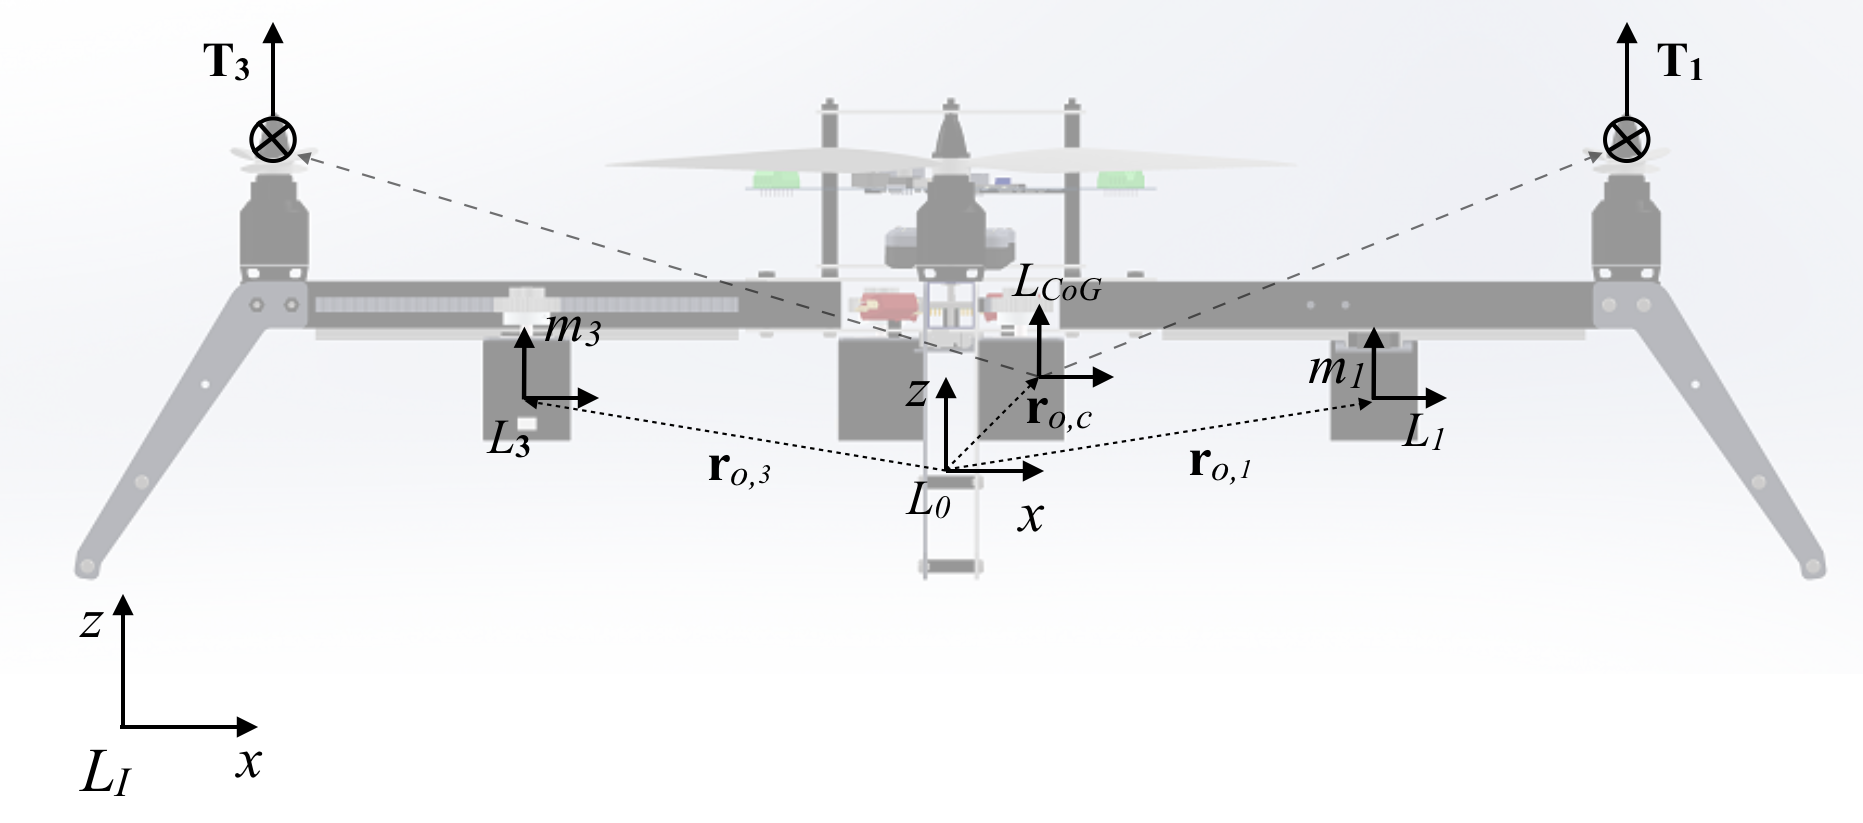
\includegraphics[scale=0.23]{model}
	\caption{Koordinatni sustav letjelice \cite{haus1}}
	\label{fig:mod}
\end{figure}

Matematičko modeliranje započinje se standardnim zapisom formule za proizvoljni vektor promjenjive duljine izražen u lokalnom mobilnom koordinatnom susavu letjelice ($L_{0}$).

\begin{equation}
\frac{d^{\omega}}{dt}(\boldsymbol{r}_{0}) =  \boldsymbol{\dot{r}}_{0} + \boldsymbol{\omega} \times \boldsymbol{r}_{0} 
\label{eq:r0}
\end{equation}

\end{document}

\newpage
\section{Identifikacija parametara sustava}
%%%%%%%%%%%%%%%%%%%%%%%%%%%%%%%%

\documentclass[11pt,a4paper]{article}
\usepackage{times}
\usepackage[utf8]{inputenc}
\usepackage[croatian]{babel}
\usepackage[T1]{fontenc} % Latin Modern

%%%%%%%%%%%%%%%%%%%%%%%%%%%%%%%%


%%%%%%%%%%%%%%%%%%%%%%%%%%%%%%%%
%%%%%%%%  MATEMATICKI PAKETI %%%%%%%%%%%
%%%%%%%%%%%%%%%%%%%%%%%%%%%%%%%%

\usepackage{amsmath}
\usepackage{amsfonts}
\usepackage{amssymb}
\usepackage{esvect}


%%%%%%%%%%%%%%%%%%%%%%%%%%%%%%%%

%%%%%%%%%%%%%%%%%%%%%%%%%%%%%%%%
%%%%%%%%%% PAKETI ZA SLIKE  %%%%%%%%%%%%
%%%%%%%%%%%%%%%%%%%%%%%%%%%%%%%%

\usepackage{graphicx}
\usepackage{float}
\usepackage[hidelinks]{hyperref}
\usepackage{caption}
\usepackage{subcaption}
\usepackage{booktabs}
\usepackage{mwe}

%%%%%%%%%%%%%%%%%%%%%%%%%%%%%%%%

%%%%%%%%%%%%%%%%%%%%%%%%%%%%%%%%
%%%%%%%%%    PRORED 1.5   %%%%%%%%%%%%%%
%%%%%%%%%%%%%%%%%%%%%%%%%%%%%%%%

\renewcommand{\baselinestretch}{1.5}

%%%%%%%%%%%%%%%%%%%%%%%%%%%%%%%%


%%%%%%%%%%%%%%%%%%%%%%%%%%%%%%%%
%%%%%%%%%% TABLICA - ANTUN %%%%%%%%%%%%
%%%%%%%%%%%%%%%%%%%%%%%%%%%%%%%%

\usepackage{array}
\usepackage{multirow}
\newcolumntype{C}[1]{>{\centering\let\newline\\\arraybackslash\hspace{0pt}}m{#1}}
\newcolumntype{L}[1]{>{\raggedright\let\newline\\\arraybackslash\hspace{0pt}}m{#1}}
\newcolumntype{R}[1]{>{\raggedleft\let\newline\\\arraybackslash\hspace{0pt}}m{#1}}
\usepackage{ctable}

%%%%%%%%%%%%%%%%%%%%%%%%%%%%%%%%

%%%%%%%%%%%%%%%%%%%%%%%%%%%%%%%%
%%%%%%%%%% TABLICA - MARTINA %%%%%%%%%%%
%%%%%%%%%%%%%%%%%%%%%%%%%%%%%%%%

\makeatletter
\renewcommand*\env@matrix[1][\arraystretch]{%
  \edef\arraystretch{#1}%
  \hskip -\arraycolsep
  \let\@ifnextchar\new@ifnextchar
  \array{*\c@MaxMatrixCols c}}
\makeatother



%%%% LATEX KOD ZA KORISTENJE TABLICE %%%%
%%% PRIMJER %%%

%\setlength\extrarowheight{1pt}
%\begin{table}[h]
%\centering
%\caption{Tablica s prikazom }
%\label{prva}
%\begin{tabular}{|l|c|}
%\hline
%\textbf{txt} &  \\ \hline 
%txt & txt    \\ 
%txt & txt   \\ \hline
%txt & txt    \\ \hline
%\end{tabular}
%\end{table}

%%%%%%%%%%%%%%%%%%%%%%%%%%%%%%%%


%%%%%%%%%%%%%%%%%%%%%%%%%%%%%%%%
%%%%%%% DIO ZA UNOS ISJECAKA KODA %%%%%%%%
%%%%%%%%%%%%%%%%%%%%%%%%%%%%%%%%

\usepackage{listings}
\usepackage{color}
 
\definecolor{codegreen}{rgb}{0,0.6,0}
\definecolor{codegray}{rgb}{0.5,0.5,0.5}
\definecolor{codepurple}{rgb}{0.58,0,0.82}
 
\lstdefinestyle{mystyle}{   
    commentstyle=\color{codegreen},
    keywordstyle=\color{blue},
    numberstyle=\tiny\color{codegray},
    stringstyle=\color{codepurple},
    basicstyle=\footnotesize,
    breakatwhitespace=false,         
    breaklines=true,                 
    captionpos=b,                    
    keepspaces=true,                 
    numbers=left,                    
    numbersep=5pt,                  
    showspaces=false,                
    showstringspaces=false,
    showtabs=false,                  
    tabsize=1
}
 
\lstset{style=mystyle}

%\lstinputlisting[language=Matlab, firstline=1, lastline=4, numbers=left, frame=single, label={lst:prvi}, caption={Diskretizacija sustava korištenjem Matlaba}, captionpos=b]{peti.m} 

%%%%%%%%%%%%%%%%%%%%%%%%%%%%%%%%


%----------------------------
% za uredjenje stranice
\usepackage[left=2.5cm,right=2.5cm,top=2.5cm,bottom=2.5cm]{geometry}
\usepackage{fancyhdr}
\pagestyle{fancy} 
\lhead{\leftmark}
\rhead{\rightmark}
\usepackage{titlesec} %za točku iza broja sectiona
\titleformat{\section}{\huge\bfseries}{\thetitle.\quad}{0em}{}
\titleformat{\subsection}{\LARGE\bfseries}{\thetitle.\quad}{0em}{}
\titleformat{\subsubsection}{\Large\bfseries}{\thetitle.\quad}{0em}{}
\titleformat{\paragraph}
{\normalfont\large\bfseries}{\thetitle.\quad}{1em}{}
\titlespacing*{\paragraph}
{0pt}{3.25ex plus 1ex minus .2ex}{1.5ex plus .2ex}
\setcounter{secnumdepth}{5}

\usepackage{indentfirst} %uvlacenje prvog paragrafa
% primjer pozivanja sectiona
% \section*{UVOD} \pdfbookmark{UVOD}{section:UVOD}

\usepackage{tocloft}
\usepackage{import}
\usepackage{standalone}
\graphicspath{{Identifikacija/figures/}} 

\hypersetup{
  colorlinks   = true, %Colours links instead of ugly boxes
  urlcolor     = black, %Colour for external hyperlinks
  linkcolor    = black, %Colour of internal links
  citecolor   = blue %Colour of citations
}

\usepackage{subcaption}
\usepackage{lscape}
\begin{document}

Određivanje parametara neizostavan je dio postupka modeliranja svakog sustava. Većinu parametara, kao što su masa i duljina, određuje se izravnim metodama, kao što su vaganje i mjerenje. Ostale parametre potrebno je odrediti eksperimentalnim putem. U prethodnom poglavlju izvedena je prijenosna funkcija modela (\ref{eq:tf}) u ovisnosti o parametrima $\zeta_{mm}$, $\omega_{mm}$ i $I_{yy}$, odnosno u ovisnosti o prigušenju sustava, nazivnoj frekvenciji i momentu tromosti (pomične mase). Ti su parametri nepoznati te ih je potrebno identificirati. 

\medskip

Identifikacija sustava je postupak određivanja matematičkog modela sustava, kao i njegovih parametara, na temelju mjerenja ulazno/izlaznih signala sustava. Odnosno to je eksperimentalna analiza sustava \cite{te}. Iako je matematički model izveden za sustav u letu, identifikacija parametara napravljena je na temelju eksperimenata provedenih na stalku s jednom osi rotacije. Unatoč provedbi eksperimenata na jednoj osi, dinamika je kvalitativno slična sustavu u letu \cite{haus3}.

\subsection{Identifikacija dinamike pokretnih masa}

Identifikaciju parametara započinjemo odabirom modela. Pretpostavlja se kako dinamika koračnog sustava masa prati $PT_{2}S$ ponašanje (\ref{eq:pt2s}). $PT_{2}S$ član je sustav drugog reda s konjugirano-kompleksnim parom polova i bez nula \cite{aupr}. Za potrebe identifikacije izrađena je \textit{Matlab Simulink shema} koja ostvaruje ponašanje algoritma upravljanja pozicijom motora pokretanog na \textit{STM} kontroleru. U shemi su postavljeni generatori pulsa koji simuliraju takt vremenskog brojača (\textit{timer-a}) na \textit{STM} kontroleru. Na temelju toga se u određenim vremenskim trenutcima generira impuls koji simulira korak okreta motora. U slučaju da se motor mora gibati većom brzinom, pulsevi se generiraju češće. 400 pulseva jednako je \textit{8 cm} hoda motora. Odziv sustava, odnosno dinamike mase koju je potrebno identificirati, prikazan je Slikom \ref{fig:masa} u nastavku:

\begin{figure}[H]
	\centering
	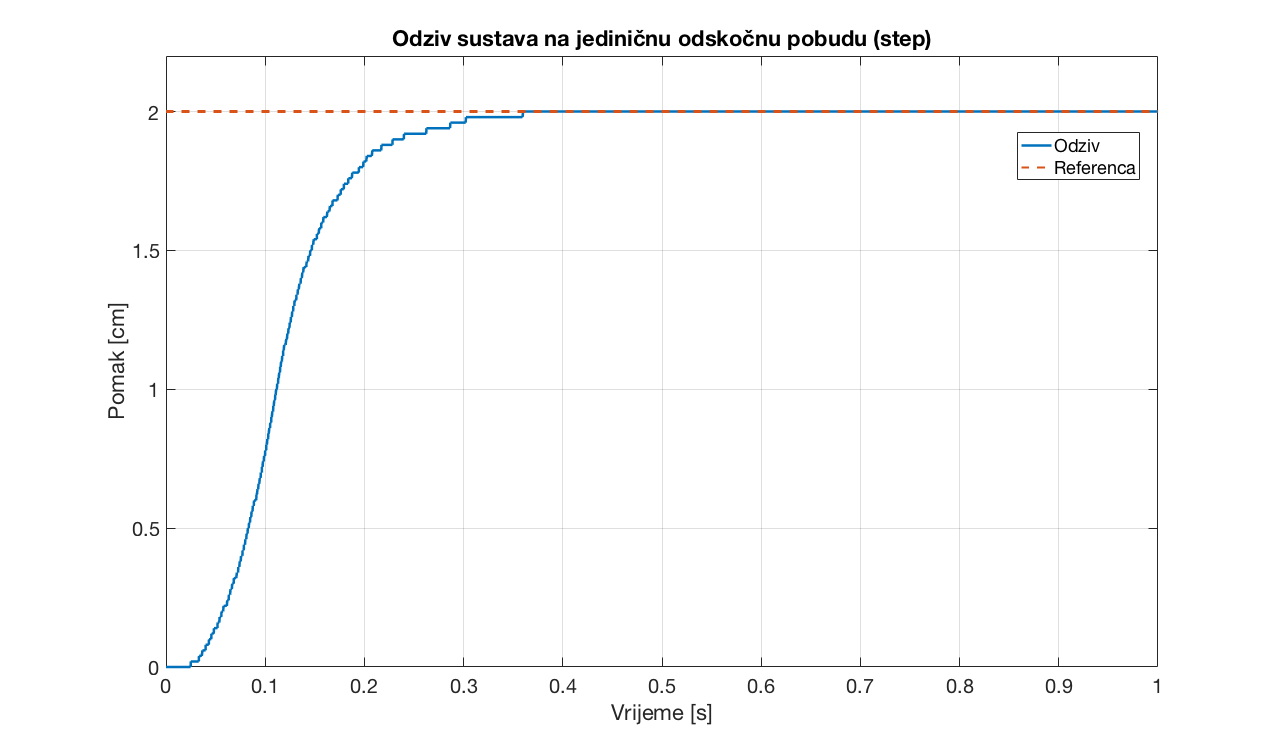
\includegraphics[width=\textwidth]{dinamika_masa}
	\caption{Dinamika pomične mase}
	\label{fig:masa}
\end{figure}


Identifikacija započinje proračunom relativnog koeficijenta prigušenja $\zeta_{mm}$. $\zeta_{mm}$ je glavni čimbenik u $PT_{2}S$ članu koji određuje oscilatornost sustava, dok prirodna frekvencija neprigušenih oscilacija $\omega_{n}$ određuje brzinu odziva sustava \cite{aupr}. Pozivom \textit{Matlab} naredbe \textit{stepinfo} na izlazni signal sustava, dobije se informacija o vremenima porasta (\ref{eq:tr}), prvog maksimuma (\ref{eq:tm}) te smirivanja (\ref{eq:te}) koji su potrebni za daljnji proračun parametara. 

\medskip

Vrijeme porasta $t_{r}$ definira se kao vrijeme za koje prijelazna funkcija \textit{y} poraste od vrijednosti $0.1y(\infty)$ na vrijednost $0.9y(\infty)$, gdje $y(\infty)$ označava vrijednost koju funkcija \textit{y} poprima u stacionarnom stanju (njezina konačna vrijednost) te se računa prema izrazu (\ref{eq:tr}):
\begin{equation}
t_{r} \approx \frac{1.8}{\omega_{mm}}
\label{eq:tr}
\end{equation}


Vrijeme prvog maksimuma $t_{m}$ je vrijeme pri kojem se pojavljuje prvo maksimalno nadvišenje:
\begin{equation}
t_{m} = \frac{\pi}{\omega_{mm}\sqrt{1 - \zeta_{mm}^{2}}}
\label{eq:tm}
\end{equation}

Vrijeme smirivanja (ustaljivanja) $t_{1\%}$ određuje trajanje prijelaznog procesa nakon kojega $y$ odstupa od zadanog iznosa za $1\%$:
\begin{equation}
t_{1\%} \approx \frac{4.6}{\zeta_{mm} \cdot \omega_{mm}}
\label{eq:te}
\end{equation}

Na temelju prethodnih jednadžbi intuitivno je jasno kako se pomnim odabirom fizikalno prihvatljivih parametara $\omega_{mm}$ i $\zeta_{mm}$ može dobiti željeno vladanje sustava. Kombinacijom jednadžbi (\ref{eq:tr}) i (\ref{eq:te}) slijedi izraz za proračun prigušenja $\zeta_{mm}$:
\begin{equation}
\zeta_{mm} = 2.556 \frac{t_{r}}{t_{1\%}}
\label{eq:zeta}
\end{equation}

$\omega_{mm}$ se računa koristeći preostalu jednadžbu (\ref{eq:tm}). Uz $t_{r} = 0.139 \ [s]$, $t_{m} = 0.638 \ [s]$ i $t_{1\%} = 0.383 \ [s]$ slijedi da su $\zeta_{mm} = 0.925$, a $\omega_{mm} = 12.992 \ [s^{-1}]$. Simulirajući odziv (\ref{eq:pt2s}) člana s ovim parametrima uočena je potreba za ubrzanjem dobivenog odziva. To je dovelo do dodatnog eksperimentalnog ugađanja parametra $\omega_{mm}$ koji direktno utječe na brzinu odziva, te je on u konačnici jedak $\omega_{mm} = 17.992 \ [s^{-1}]$. Identificirana dinamika pomičnih masa prikazana je Slikom \ref{fig:masa_din}, dok je konačna prijenosna funkcija jednaka (\ref{eq:mase_tf}):

\begin{equation}
\boxed{
\frac{x_{i}}{x_{i, ref}}(s) = \frac{1}{3.098\cdot10^{-3}s^{2} + 0.103 s + 1}
}
\label{eq:mase_tf}
\end{equation}

\begin{figure}[H]
	\centering
	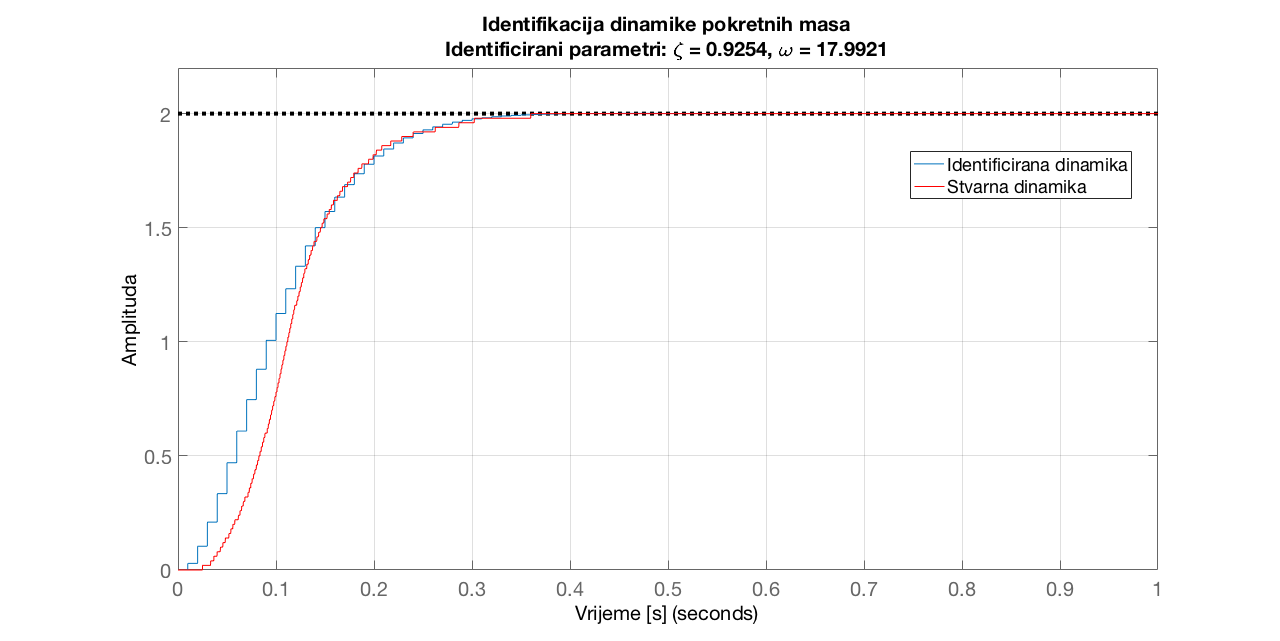
\includegraphics[width=\textwidth]{mase_dinam}
	\caption{Identificirana dinamika pokretnih masa}
	\label{fig:masa_din}
\end{figure}

\subsection{Identifikacija momenta tromosti}

Moment tromosti je mjera tromosti tijela pri rotaciji. On utječe na rotaciju kao što masa utječe na translaciju materijalne točke, stoga ga je izrazito bitno točno identificirati \cite{fiz1}. Određuje se eksperimentalnim putem. 

\medskip

Postupak započinje postavljanjem letjelice na stalak s jednom osi rotacije (\textit{single axis gimbal}). Prvo se provodi eksperiment za \textit{kut poniranja}, a potom za \textit{kut valjanja}. Letjelica se postavlja u horizontalni položaj, tako da je iznos kuta jednak nula, dok se mase postavljaju u proizvoljni krajnji položaj (lijevo ili desno). Potom se letjelica pušta iz početnog položaja te se odzivi snimaju za daljnju identifikaciju. 

\begin{figure}[H]
	\centering
	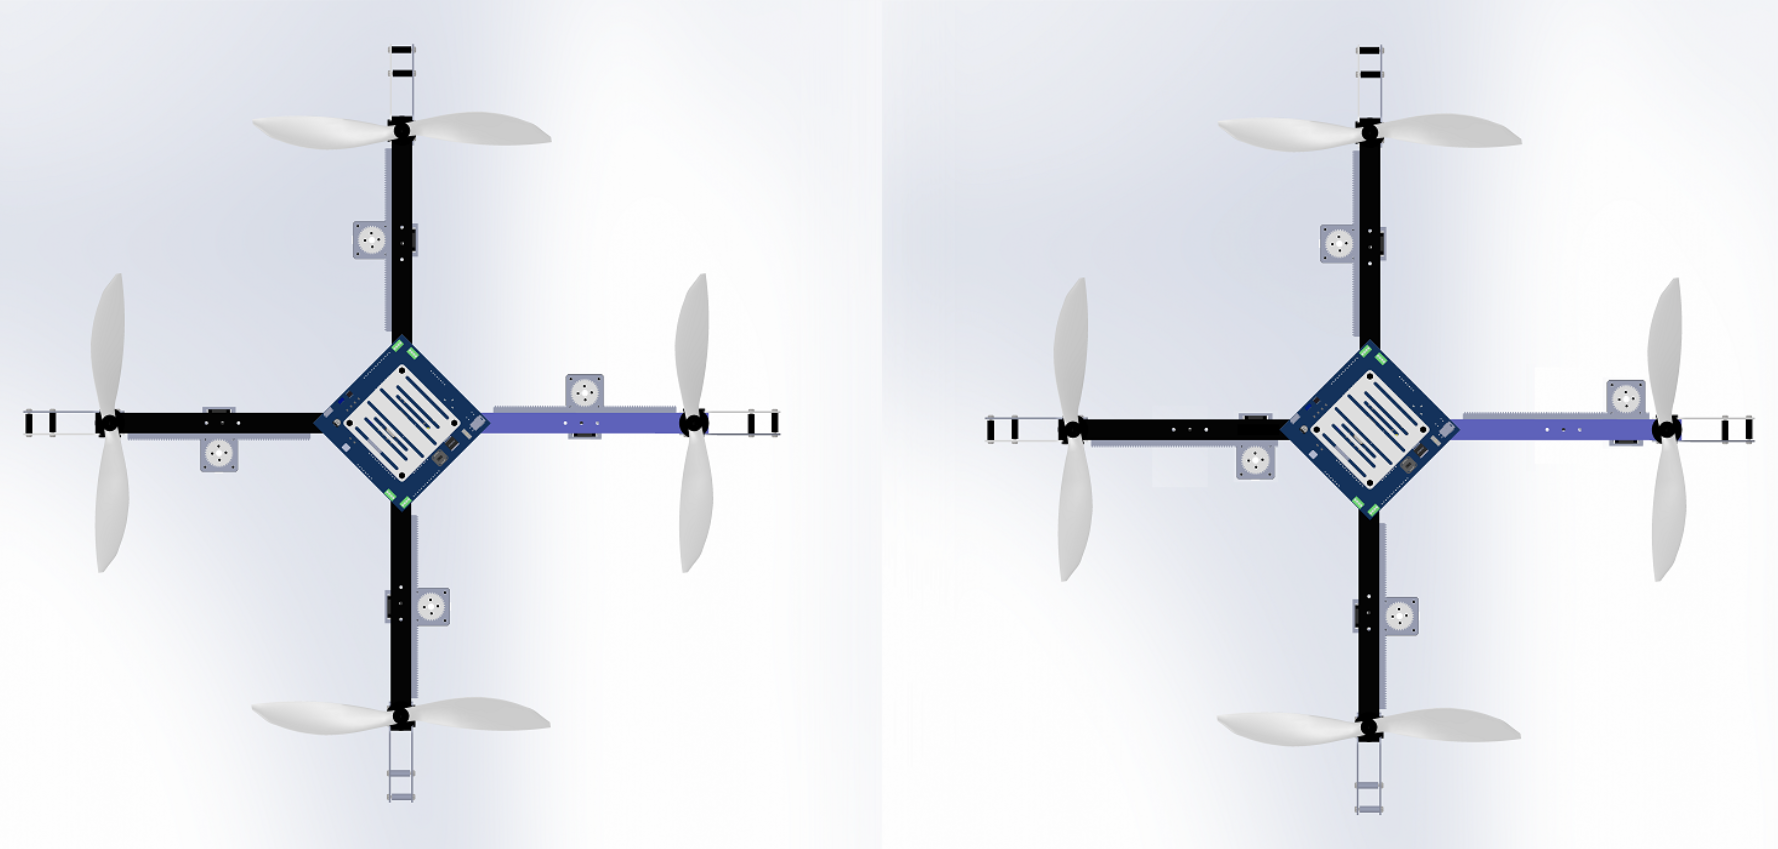
\includegraphics[scale=0.2]{pomak}
	\caption{Prikaz pomaka pomičnih masa za $\Delta x = 8 \ cm$ u svrhu identifikacije momenta tromosti}
	\label{fig:}
\end{figure}


\medskip

U tako kontroliranom okruženju, na letjelicu ne djeluju vanjski poremećaji već samo sila gravitacije. Stoga u izrazu (\ref{eq:Iyyw}) ostaje samo prvi član, dok su ostali jednaki nula:
\begin{equation}
I_{yy} \dot{\omega}_{y} = \sum_{j=1}^{4} M_{fj}  =  \sum_{j=1}^{4} r_{c,j} \times F_{r,j}
\label{eq:Iyyw2}
\end{equation}

gdje su:
\begin{equation}
F_{r,1} = F_{r,2} = F_{r,3} = F_{r,4} = \frac{F_{g}}{4} = \frac{Mg}{4}
\label{eq:F1234}
\end{equation}

\begin{equation}
r_{c1,x} = \ell + \Delta \ell \  \  , \ r_{c2,x} = \Delta \ell \  \ , \  r_{c3,x} = \ell - \Delta x \  \ , \  r_{c4,x} =  \Delta x
\label{eq:rcj}
\end{equation}

gdje je $\Delta \ell = \mu(x_{1}  + x_{3})$.

Uvrštavanjem (\ref{eq:Fg}),(\ref{eq:F1234}) i (\ref{eq:rcj}) u (\ref{eq:Iyyw2}) slijedi:
\begin{equation}
 I_{yy}\dot{\omega}_{y} = mg(x_{1} + x_{3})
 \label{eq:Iyyw3}
 \end{equation} 
 
 Ali s obzirom da se mase pomiču za jednaku vrijednost, vrijedi jednakost:
 \begin{equation}
 x_{1} = x_{3} = 2\cdot\Delta x
 \label{eq:x1xx3}
 \end{equation}
pa slijedi:
\begin{equation}
I_{yy} \dot{\omega}_{y} = 2mg\Delta x = u
\label{eq:upr}
\end{equation}

Prelaskom u Laplaceovu domenu, te izražavanjem parametra $\omega_{y}$ koji je poznat iz snimljenih odziva, slijedi sustav koji je potrebno modelirati, odnosno koji se koristi pri identifikaciji:
\begin{equation}
\omega_{y} = \frac{2mg \Delta x}{I_{yy}} \frac{1}{s} = \frac{u}{I_{yy}} \frac{1}{s} = u \cdot K_{identif.} \cdot \frac{1}{s}
\label{eq:wy}
\end{equation}
\medskip
gdje je $K_{identif.}$ nepoznati parametar koji se identificira te je jednak $\frac{1}{I_{yy}}$, dok je $u$ poznati upravljački signal koji se koristi kao pobuda sustava identifikacije.

Identifikacija se provodi u programskom okruženju \textit{Matlab} koristeći \textit{fminsearch} funkciju kojom je implementirana \textit{Simplex metoda optimiranja} \cite{fmin}. Eksperimentalna analiza ponovljena je na četiri skupa mjerenja, identificirani odzivi i parametri prikazani su Slikom \ref{fig:Iyy}:  
    



\begin{figure}[H]
	\centering
	\begin{subfigure}{.5\textwidth}
		\centering
		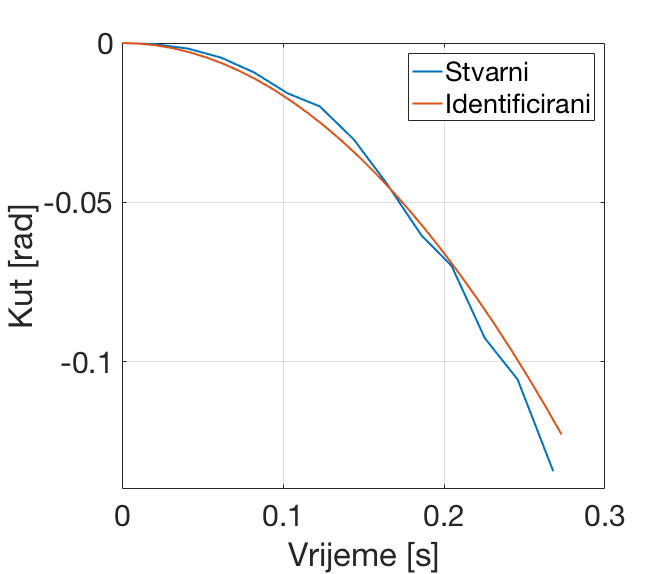
\includegraphics[width=1\linewidth]{1}
		\caption{$I_{yy} = 0.0990 \ kg \cdot m^{2}$}
		\label{fig:mj1}
	\end{subfigure}%
	\begin{subfigure}{.5\textwidth}
		\centering
		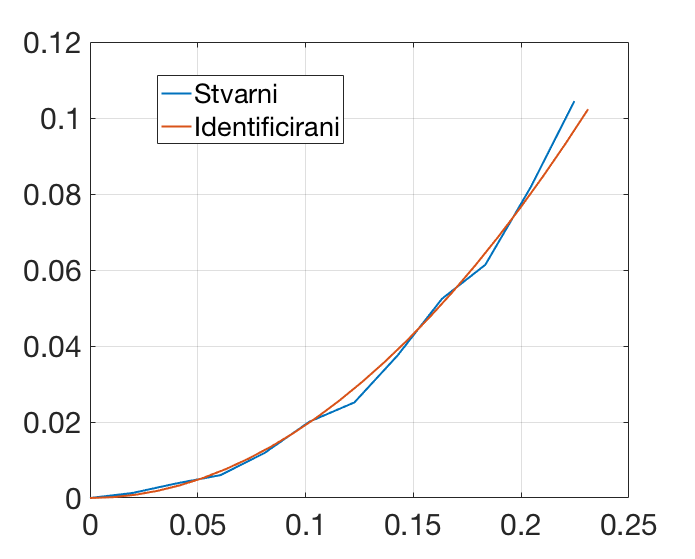
\includegraphics[width=1\linewidth]{2}
		\caption{$I_{yy} = 0.08515 \ kg \cdot m^{2}$}
		\label{fig:mj2}
	\end{subfigure}
	\begin{subfigure}{.5\textwidth}
		\centering
		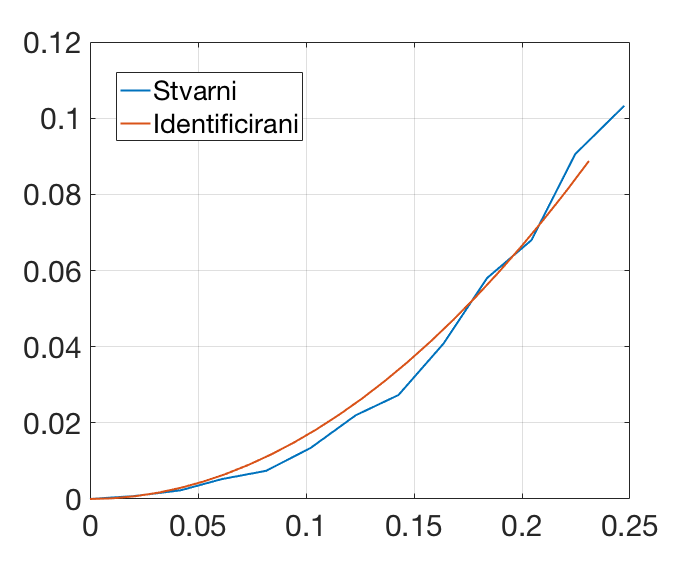
\includegraphics[width=1\linewidth]{3}
		\caption{$I_{yy} = 0.0981 \ kg \cdot m^{2}$}
		\label{fig:mj3}
	\end{subfigure}%
	\begin{subfigure}{.5\textwidth}
		\centering
		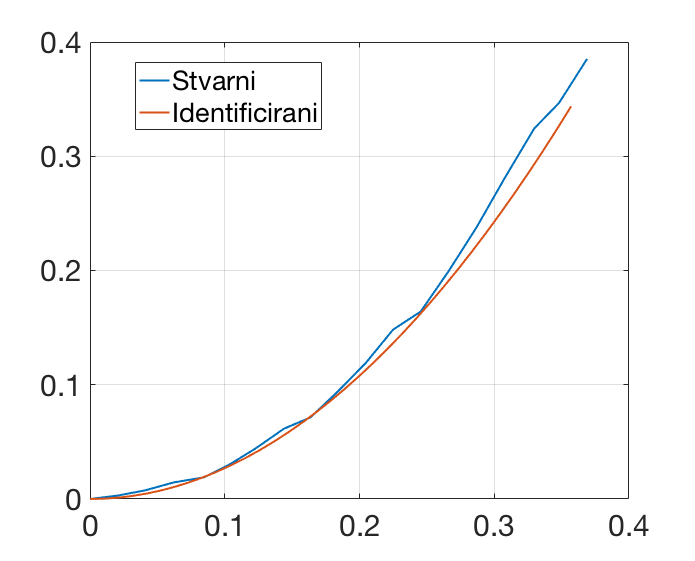
\includegraphics[width=1\linewidth]{4}
		\caption{$I_{yy} = 0.06055 \ kg \cdot m^{2}$}
		\label{fig:mj4}
	\end{subfigure}
	
	\caption{Rezultat identifikacije momenta tromosti}
	\label{fig:Iyy}
\end{figure} 



Konačan iznos momenta tromosti $I_{yy}$ odabiremo kao srednju vrijednost dobivenih rezultata:

\begin{equation}
\boxed{
I_{yy} = 0.0857 \ kg \cdot m^{2}
}
\label{eq:Iyy}
\end{equation}


\newpage

\subsection{Parametri modela letjelice}




\setlength\extrarowheight{1pt}
\begin{table}[h]
\centering
\caption{Parametri modela letjelice}
\label{params}
\begin{tabular}{lll}
\hline
\textbf{Oznaka} &  \textbf{Iznos}  &  \textbf{Opis}   \\ \hline 
$I_{xx}$ & $0.0857 \ kgm^{2}$ & Moment tromosti cijelog sustava letjelice (\textit{kut valjanja})   \\ 
$I_{yy}$ & $0.0857 \ kg m^{2}$ &  Moment tromosti cijelog sustava letjelice (\textit{kut poniranja})\\ 
$m$ & $0.208 \ kg$ &  Masa pokretne mase    \\ 
$M$ & $2.083 \ kg$ & Ukupna masa letjelice      \\ 
$b_{f}$ & $8.54858e-6 \ kgm$& Konstanta potiska motora     \\ 
$b_{m}$ & $0.01$& Momentna konstanta motora     \\ 
$ L$ & $0.2520 \ m $ &  Duljina kraka letjelice    \\ 
$\omega_{mm} $ & $ 17.9921 \ rad\/s$ & Nazivna frekvencija kliznog mehanizma pokretnih masa     \\
$\zeta_{mm} $ & $ 0.9254 \ rad\/s$ & Faktor prigušivanja kliznog mehanizma pokretnih masa      \\  
$T_{r} $ & $ 0.2 \ s$ &  Vremenska konstanta rotora    \\
$\Delta \ell $ & $\pm0.08 \ m $ &  Maksimalan hod pokretnih masa    \\  
$z_{m} $ & $ 0$ & Vertikalan pomak masa s obzirom na ishodište     \\ 
$T_{s} $ & $ 0.01 \ s$ &  Vrijeme uzorkovanja diskretnog sustava    \\ \hline
\end{tabular}
\end{table}



\end{document}

\newpage
\section{Upravljačka struktura}
%%%%%%%%%%%%%%%%%%%%%%%%%%%%%%%%

\documentclass[11pt,a4paper]{article}
\usepackage{times}
\usepackage[utf8]{inputenc}
\usepackage[croatian]{babel}
\usepackage[T1]{fontenc} % Latin Modern

%%%%%%%%%%%%%%%%%%%%%%%%%%%%%%%%


%%%%%%%%%%%%%%%%%%%%%%%%%%%%%%%%
%%%%%%%%  MATEMATICKI PAKETI %%%%%%%%%%%
%%%%%%%%%%%%%%%%%%%%%%%%%%%%%%%%

\usepackage{amsmath}
\usepackage{amsfonts}
\usepackage{amssymb}
\usepackage{esvect}

%%%%%%%%%%%%%%%%%%%%%%%%%%%%%%%%

%%%%%%%%%%%%%%%%%%%%%%%%%%%%%%%%
%%%%%%%%%% PAKETI ZA SLIKE  %%%%%%%%%%%%
%%%%%%%%%%%%%%%%%%%%%%%%%%%%%%%%

\usepackage{graphicx}
\usepackage{float}
\usepackage[hidelinks]{hyperref}
\usepackage{caption}
\usepackage{subcaption}
\usepackage{booktabs}

%%%%%%%%%%%%%%%%%%%%%%%%%%%%%%%%

%%%%%%%%%%%%%%%%%%%%%%%%%%%%%%%%
%%%%%%%%%    PRORED 1.5   %%%%%%%%%%%%%%
%%%%%%%%%%%%%%%%%%%%%%%%%%%%%%%%

\renewcommand{\baselinestretch}{1.5}

%%%%%%%%%%%%%%%%%%%%%%%%%%%%%%%%


%%%%%%%%%%%%%%%%%%%%%%%%%%%%%%%%
%%%%%%%%%% TABLICA - ANTUN %%%%%%%%%%%%
%%%%%%%%%%%%%%%%%%%%%%%%%%%%%%%%

\usepackage{array}
\usepackage{multirow}
\newcolumntype{C}[1]{>{\centering\let\newline\\\arraybackslash\hspace{0pt}}m{#1}}
\newcolumntype{L}[1]{>{\raggedright\let\newline\\\arraybackslash\hspace{0pt}}m{#1}}
\newcolumntype{R}[1]{>{\raggedleft\let\newline\\\arraybackslash\hspace{0pt}}m{#1}}
\usepackage{ctable}

%%%%%%%%%%%%%%%%%%%%%%%%%%%%%%%%

%%%%%%%%%%%%%%%%%%%%%%%%%%%%%%%%
%%%%%%%%%% TABLICA - MARTINA %%%%%%%%%%%
%%%%%%%%%%%%%%%%%%%%%%%%%%%%%%%%

\makeatletter
\renewcommand*\env@matrix[1][\arraystretch]{%
  \edef\arraystretch{#1}%
  \hskip -\arraycolsep
  \let\@ifnextchar\new@ifnextchar
  \array{*\c@MaxMatrixCols c}}
\makeatother



%%%% LATEX KOD ZA KORISTENJE TABLICE %%%%
%%% PRIMJER %%%

%\setlength\extrarowheight{1pt}
%\begin{table}[h]
%\centering
%\caption{Tablica s prikazom }
%\label{prva}
%\begin{tabular}{|l|c|}
%\hline
%\textbf{txt} &  \\ \hline 
%txt & txt    \\ 
%txt & txt   \\ \hline
%txt & txt    \\ \hline
%\end{tabular}
%\end{table}

%%%%%%%%%%%%%%%%%%%%%%%%%%%%%%%%


%%%%%%%%%%%%%%%%%%%%%%%%%%%%%%%%
%%%%%%% DIO ZA UNOS ISJECAKA KODA %%%%%%%%
%%%%%%%%%%%%%%%%%%%%%%%%%%%%%%%%

\usepackage{listings}
\usepackage{color}
 
\definecolor{codegreen}{rgb}{0,0.6,0}
\definecolor{codegray}{rgb}{0.5,0.5,0.5}
\definecolor{codepurple}{rgb}{0.58,0,0.82}
 
\lstdefinestyle{mystyle}{   
    commentstyle=\color{codegreen},
    keywordstyle=\color{blue},
    numberstyle=\tiny\color{codegray},
    stringstyle=\color{codepurple},
    basicstyle=\footnotesize,
    breakatwhitespace=false,         
    breaklines=true,                 
    captionpos=b,                    
    keepspaces=true,                 
    numbers=left,                    
    numbersep=5pt,                  
    showspaces=false,                
    showstringspaces=false,
    showtabs=false,                  
    tabsize=1
}
 
\lstset{style=mystyle}

%\lstinputlisting[language=Matlab, firstline=1, lastline=4, numbers=left, frame=single, label={lst:prvi}, caption={Diskretizacija sustava korištenjem Matlaba}, captionpos=b]{peti.m} 

%%%%%%%%%%%%%%%%%%%%%%%%%%%%%%%%


%----------------------------
% za uredjenje stranice
\usepackage[left=2.5cm,right=2.5cm,top=2.5cm,bottom=2.5cm]{geometry}
\usepackage{fancyhdr}
\pagestyle{fancy} 
\lhead{\leftmark}
\rhead{\rightmark}
\usepackage{titlesec} %za točku iza broja sectiona
\titleformat{\section}{\huge\bfseries}{\thetitle.\quad}{0em}{}
\titleformat{\subsection}{\LARGE\bfseries}{\thetitle.\quad}{0em}{}
\titleformat{\subsubsection}{\Large\bfseries}{\thetitle.\quad}{0em}{}
\titleformat{\paragraph}
{\normalfont\large\bfseries}{\thetitle.\quad}{1em}{}
\titlespacing*{\paragraph}
{0pt}{3.25ex plus 1ex minus .2ex}{1.5ex plus .2ex}
\setcounter{secnumdepth}{5}

\usepackage{indentfirst} %uvlacenje prvog paragrafa
% primjer pozivanja sectiona
% \section*{UVOD} \pdfbookmark{UVOD}{section:UVOD}

\usepackage{tocloft}
\usepackage{import}
\usepackage{standalone}
\graphicspath{{Identifikacija/figures/}} 

\hypersetup{
  colorlinks   = true, %Colours links instead of ugly boxes
  urlcolor     = black, %Colour for external hyperlinks
  linkcolor    = black, %Colour of internal links
  citecolor   = blue %Colour of citations
}

\usepackage{subcaption}
\usepackage{lscape}
\begin{document}

Cilj modeliranja ovog sustava jest biti u mogućnosti u konačnici tim sustavom upravljati. Postoje jednopetljaste i višepetljaste strukture upravljanja. Jednopetljastim strukturama upravljanja često nije moguće postići visoke performanse upravljanja složenim sustavima zato što se složenim sustavom nastoji upravljati na temelju samo jedne informacije o sustavu. Stoga, regulator na promjene u sustavu reagira tek nakon što se njihov efekt registrira na iznosu izlazne veličine. Iz tog razloga značajnu primjenu imaju višepetljaste strukture upravljanja, odnosno strukture \textit{kaskadnog} upravljanja. Osnovna ideja kaskadnog upravljanja jest uz primarnu reguliranu veličinu uvesti dodatne, pomoćne, izlazne veličine. Time bi se omogućila brža reakcija sustava upravljanja na djelovanje poremećajne veličine, prije nego li ona počne djelovati na primarnu reguliranu veličinu \cite{uemp}. Vanjska petlja je primarna petlja, dok su unutarnje pomoćne.   

\medskip

Iz navedenih razloga modelira se kaskadna upravljačka struktura za sustav letjelice s pomičnim masama. Unutarnja petlja zatvara se po kutnoj brzini, dok se vanjska petlja zatvara po poziciji, odnosno kutu. Načelna upravljačka shema prikazana je Slikom \ref{fig:upr}. 


\begin{figure}[H]
	\centering
	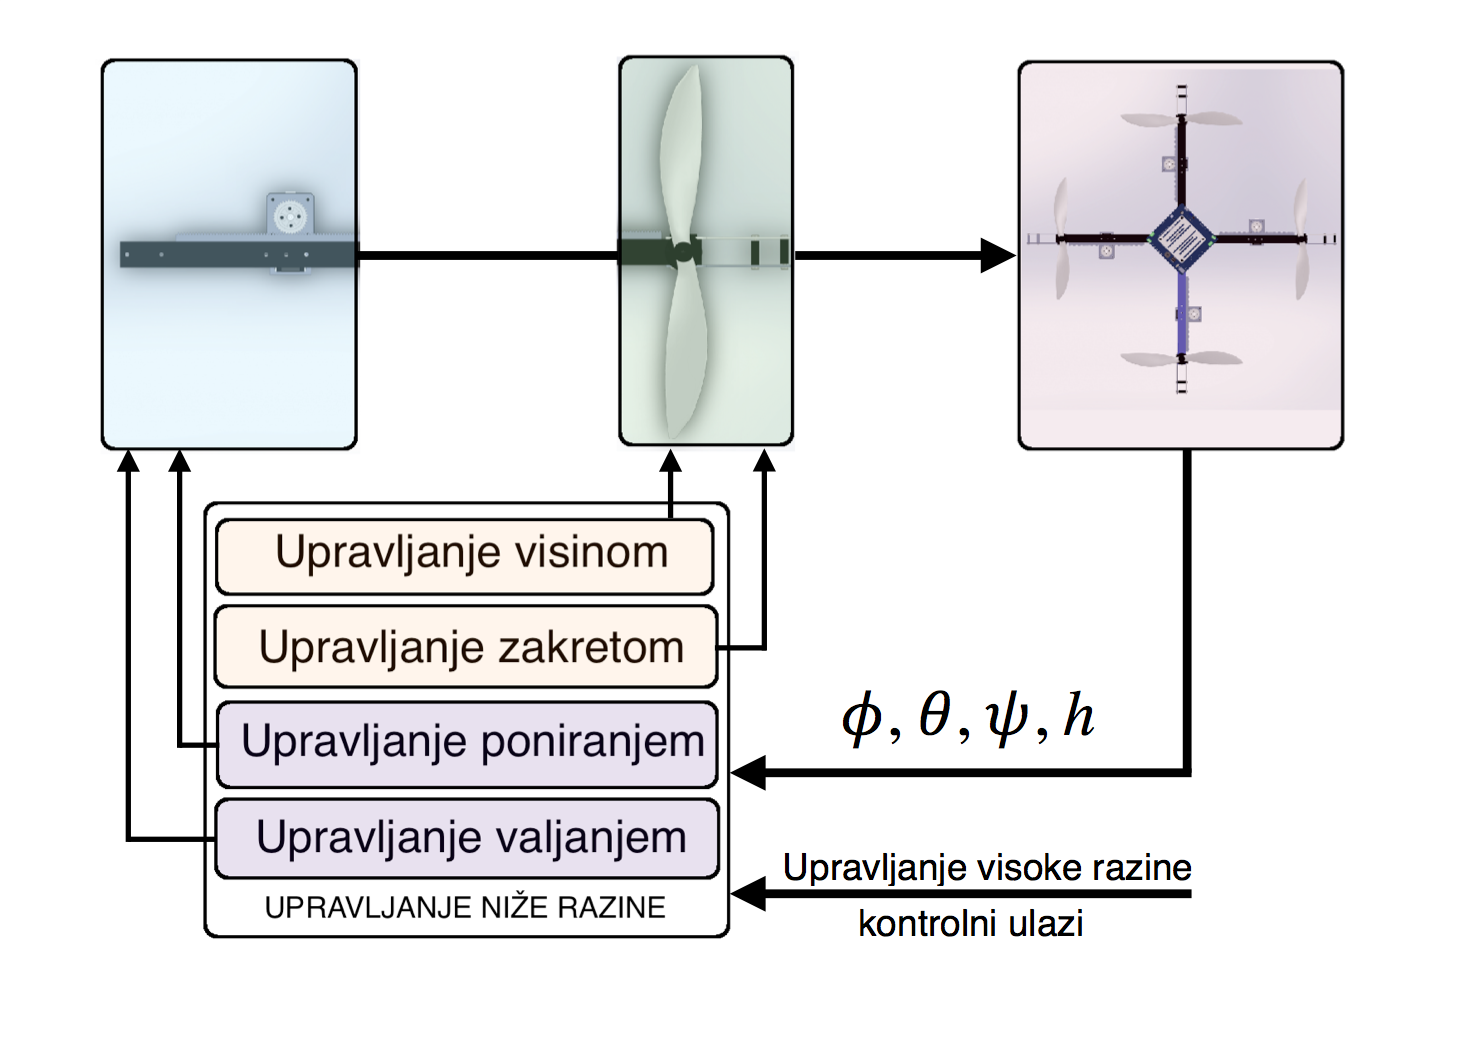
\includegraphics[width=\textwidth]{upr}
	\caption{Upravljačka struktura sustava letjelice}
	\label{fig:upr}
\end{figure}

\newpage

Modeliran je koncept i odabrana je upravljačka struktura, stoga još preostaje odabrati vrstu regulatora te proračunati njegove parametre. Odabire se \textit{P} regulator za upravljanje i unutarnjom i vanjskom petljom. Parametre regulatora, pojačanja $K_{p}$, određujemo koristeći metodu \textit{krivulje mjesta korijena}. Postupak \textit{krivulje mjesta korijena}, ili skraćeno \textit{KMK}, omogućava donošenje zaključka o vladanju zatvorenog regulacijskog kruga na temelju položaja polova i nula prijenosne funkcije otvorenog regulacijskog kruga u kompleksnoj \textit{s} ravnini. Na temelju izgleda KMK-a zaključuje se o stabilnosti zatvorenog regulacijskog kruga \cite{mato}. 

\medskip

Određivanje parametara regulatora obavlja se u dva koraka. Prvo se određuje pojačanje unutarnje petlje prema izrazu za prijenosnu funkciju otvorenog kruga sustava (\ref{eq:tf}) koristeći postupak \textit{krivulje mjesta korijena}. Zatim se određuje prijenosna funkcija zatvorenog kruga unutarnje petlje s prijenosnom funkcijom P regulatora ($K_{p}$) te s prijenosnom funkcijom procesa. Prijenosna funkcija zatvorenog kruga uz dodan integrator jednaka je prijenosnoj funkciji otvorenog kruga vanjske petlje. Za tu se prijenosnu funkciju postupak ponavlja.  

\medskip

Za određivanje \textit{krivulje mjesta korijena} unutarnje petlje koristi se prijenosna funkcija otvorenog kruga (\ref{eq:tf}) te parametri iz Tablice \ref{params}. Sustav je stabilan za sva pojačanja za koja se nule i polovi nalaze unutar jedinične kružnice.  Rezultirajući KMK prikazan je Slikom \ref{fig:unutarnja_Kp}, na kojoj je također prikazan način odabira parametra P regulatora unutarnje petlje. Na slici su prikazana dva očitanja pojačanja. Jedan se nalazi na rubu stabilnosti i jednak je $K= 0.7$. S obzirom na da je to pojačanje na rubu stabilnosti znači da ako se odabere $K_{p} > K$, sustav će postati nestabilan. Iz tog razloga odabire se pojačanje koje polove povlači unutar jedinične kružnice, prikazano drugim očitanjem. Konačan iznos pojačanja P regulatora unutarnje upravljačke petlje jednak je:

 \begin{equation}
 \boxed{
 K_{p,in} = 0.1
 } \ .
 \label{eq:Kp_in}
 \end{equation}


\begin{figure}[H]
	\centering
	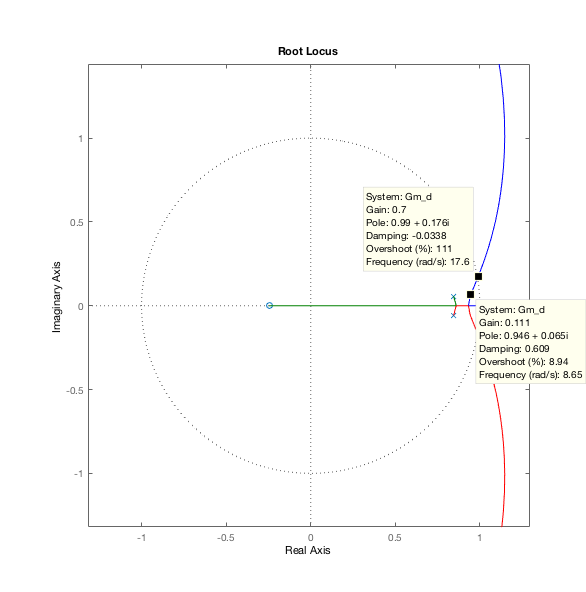
\includegraphics[scale=0.55]{unutarnja_Kp}
	\caption{Odabir pojačanja P regulatora unutarnje upravljačke petlje}
	\label{fig:unutarnja_Kp}
\end{figure}

Stabilnost zatvorenog kruga unutarnje petlje može se ispitati odzivom prijenosne funkcije tog zatvorenog kruga na jediničnu odskočnu pobudu (step) te je taj odziv prikazan Slikom \ref{fig:step1}:

\begin{figure}[H]
	\centering
	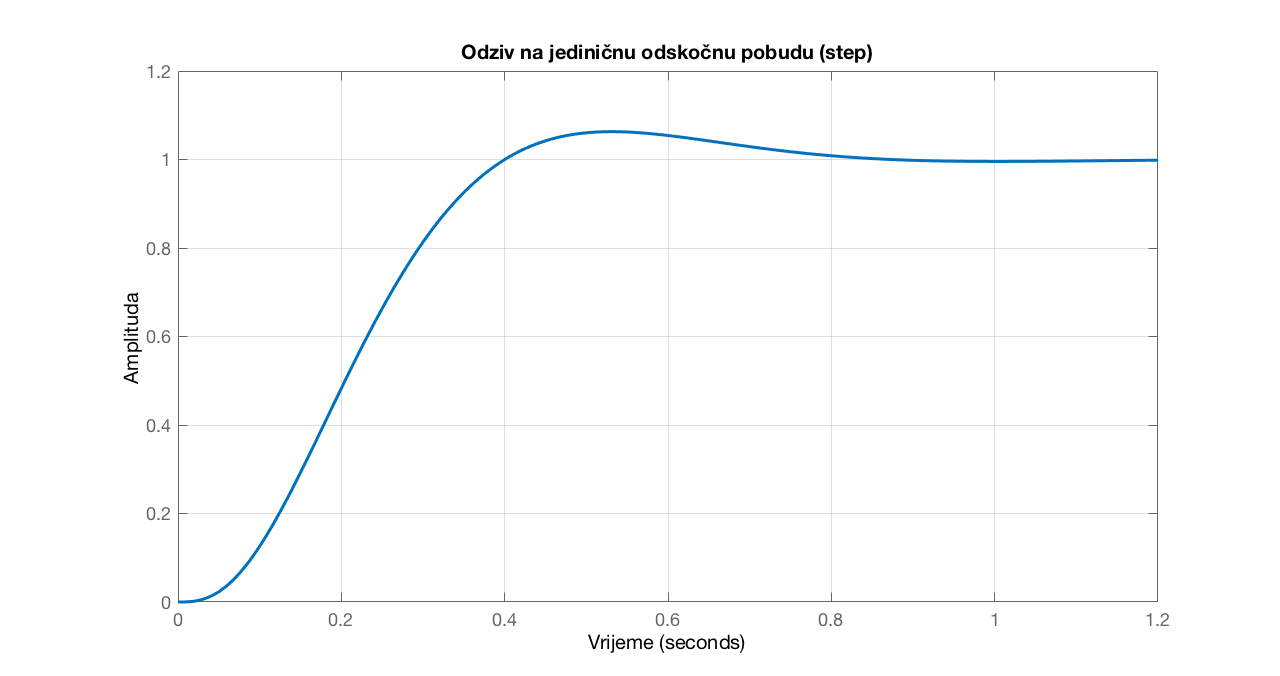
\includegraphics[width=\textwidth]{unutarnja_step}
	\caption{Odziv zatvorenog kruga unutarnje upravljačke petlje na jediničnu odskočnu pobudu}
	\label{fig:step1}
\end{figure}


Analogan postupak primjenjuje se i za vanjsku upravljačku petlju. Prijenosna funkcija otvorenog kruga vanjske petlje jednaka je prijenosnoj funkciji zatvorenog kruga unutarnje petlje uz dodatak integratora:

\begin{equation}
G_{o,out} = \frac{K_{p,in}G_{o,in}}{1 + K_{p,in}G_{o,in}} \frac{1}{s}\ ,
\label{eq:tf2}
\end{equation}

gdje je $K_{p,in} = 0.1$, a $G_{o,in}$  je jednak (\ref{eq:tf}) s uvrštenim parametrima:


\begin{equation}
G_{o,in} = \frac{1}{s(6.4875\cdot10^{-5}s^{2} + 0.0022s  + 0.0210)} \ ,
\label{eq:Goin}
\end{equation}

pa slijedi konačan izraz za $G_{o,out}$:

\begin{equation}
G_{o,out} = \frac{0.1}{6.4875\cdot10^{-5}s^{3} + 0.0022s^{2}  + 0.0210s + 0.111} \frac{1}{s} \ .
\label{eq:Ginz}
\end{equation}
\medskip
\textit{Krivulja mjesta korijena} otvorenog kruga vanjske petlje kao i odabir pojačanja P regulatora prikazano je Slikom \ref{fig:vanjska_Kp}:

\begin{figure}[H]
	\centering
	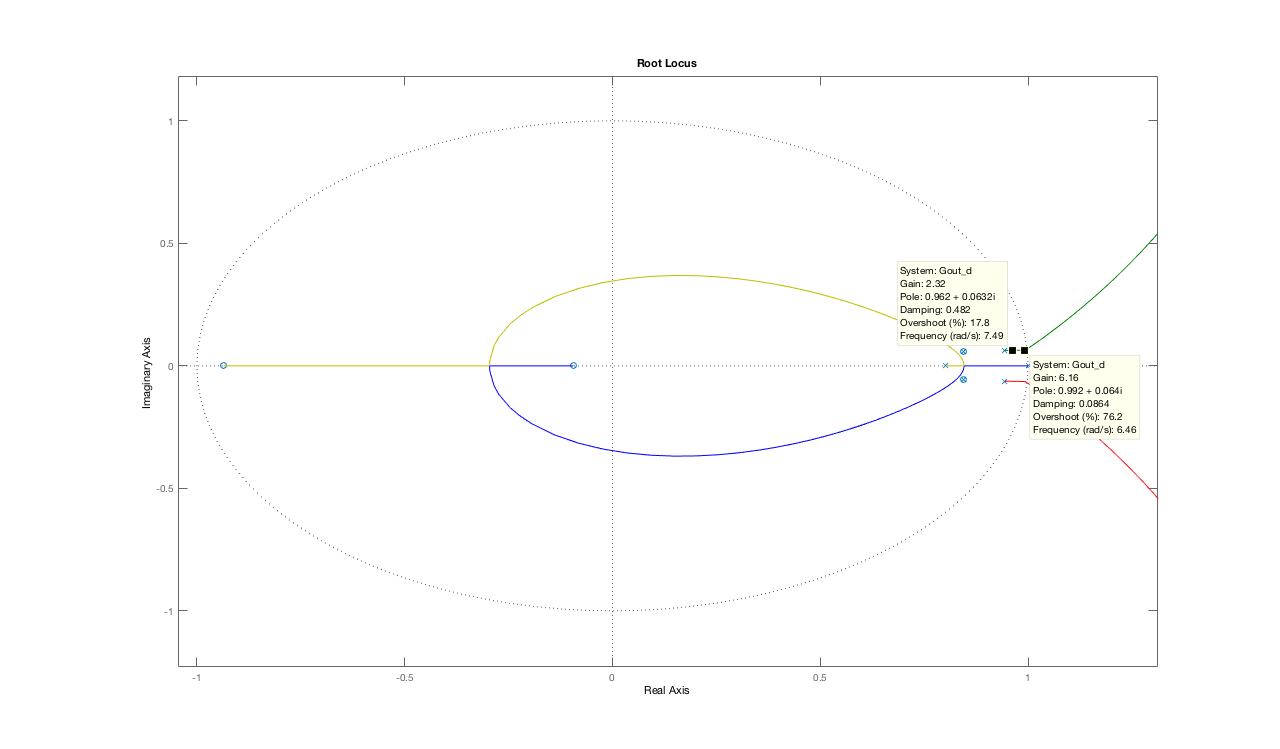
\includegraphics[width=\textwidth]{vanjska_Kp2}
	\caption{Odabir pojačanja P regulatora vanjske upravljačke petlje}
	\label{fig:vanjska_Kp}
\end{figure}

\newpage
Konačan iznos pojačanja P regulatora vanjske upravljačke petlje jednak je:
 \begin{equation}
 \boxed{
 K_{p,out} = 2.32
 } \ .
 \label{eq:Kp_out}
 \end{equation}
 
Slijedi opći zapis prijenosne funkcije zatvorenog kruga upravljanja:

\begin{equation}
G_{z,out} = \frac{K_{p,out}G_{o,out}}{1 + K_{p,out}G_{o,out}} \ .
\label{eq:Goutz}
\end{equation}
 
 Konačna prijenosna funkcija zatvorenog kruga upravljanja jednaka je:
 
 \begin{equation}
 G_{o,z} = \frac{0.232}{6.4875\cdot10^{-5}s^{4} + 0.0022s^{3}  + 0.0210s^{2} + 0.1s + 0.232} \ .
 \label{eq:Goz}
 \end{equation}

Stabilnost zatvorenog kruga vanjske petlje dokazuje se odzivom prijenosne funkcije zatvorenog kruga (\ref{eq:Goz}) na jediničnu odskočnu pobudu (step) te je taj odziv prikazan Slikom \ref{fig:step2}:

\begin{figure}[H]
	\centering
	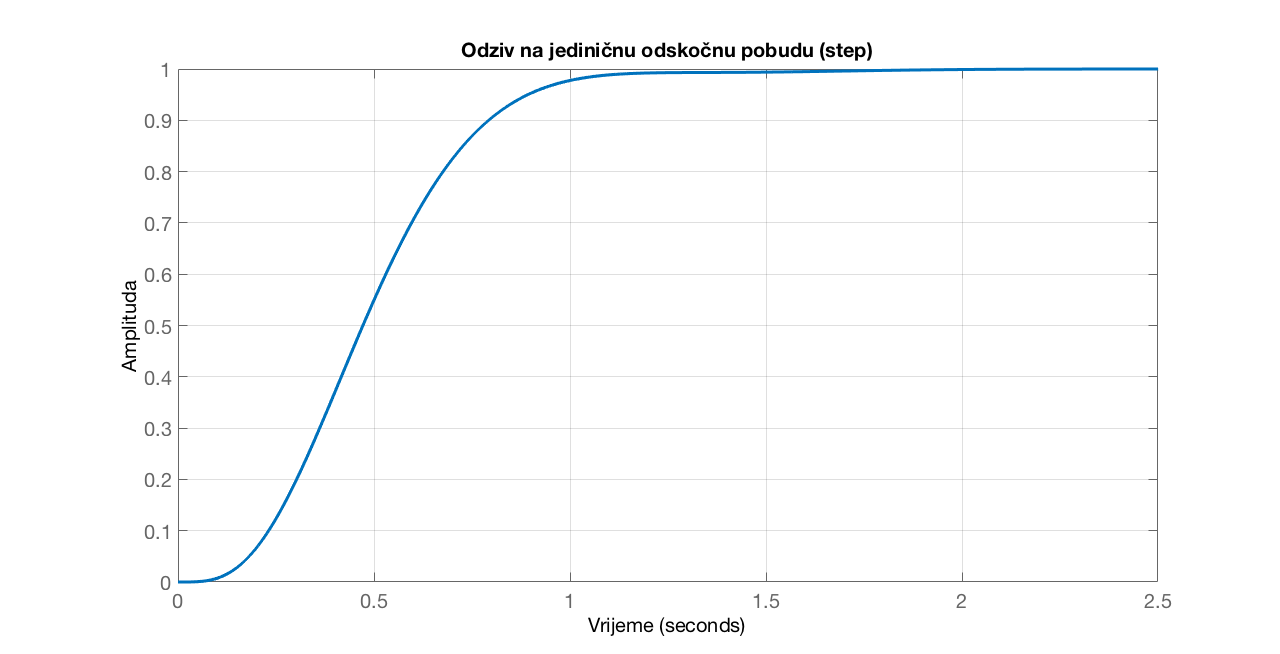
\includegraphics[width=\textwidth]{vanjska_step}
	\caption{Odziv zatvorenog kruga vanjske upravljačke petlje na jediničnu odskočnu pobudu}
	\label{fig:step2}
\end{figure}


\end{document}

\newpage
\section{Mehanička konstrukcija}
%%%%%%%%%%%%%%%%%%%%%%%%%%%%%%%%

\documentclass[11pt,a4paper]{article}
\usepackage{times}
\usepackage[utf8]{inputenc}
\usepackage[croatian]{babel}
\usepackage[T1]{fontenc} % Latin Modern

%%%%%%%%%%%%%%%%%%%%%%%%%%%%%%%%


%%%%%%%%%%%%%%%%%%%%%%%%%%%%%%%%
%%%%%%%%  MATEMATICKI PAKETI %%%%%%%%%%%
%%%%%%%%%%%%%%%%%%%%%%%%%%%%%%%%

\usepackage{amsmath}
\usepackage{amsfonts}
\usepackage{amssymb}
\usepackage{esvect}

%%%%%%%%%%%%%%%%%%%%%%%%%%%%%%%%

%%%%%%%%%%%%%%%%%%%%%%%%%%%%%%%%
%%%%%%%%%% PAKETI ZA SLIKE  %%%%%%%%%%%%
%%%%%%%%%%%%%%%%%%%%%%%%%%%%%%%%

\usepackage{graphicx}
\usepackage{float}
\usepackage[hidelinks]{hyperref}
\usepackage{caption}
\usepackage{subcaption}
\usepackage{booktabs}


%%%%%%%%%%%%%%%%%%%%%%%%%%%%%%%%

%%%%%%%%%%%%%%%%%%%%%%%%%%%%%%%%
%%%%%%%%%    PRORED 1.5   %%%%%%%%%%%%%%
%%%%%%%%%%%%%%%%%%%%%%%%%%%%%%%%

\renewcommand{\baselinestretch}{1.5}

%%%%%%%%%%%%%%%%%%%%%%%%%%%%%%%%


%%%%%%%%%%%%%%%%%%%%%%%%%%%%%%%%
%%%%%%%%%% TABLICA - ANTUN %%%%%%%%%%%%
%%%%%%%%%%%%%%%%%%%%%%%%%%%%%%%%

\usepackage{array}
\usepackage{multirow}
\newcolumntype{C}[1]{>{\centering\let\newline\\\arraybackslash\hspace{0pt}}m{#1}}
\newcolumntype{L}[1]{>{\raggedright\let\newline\\\arraybackslash\hspace{0pt}}m{#1}}
\newcolumntype{R}[1]{>{\raggedleft\let\newline\\\arraybackslash\hspace{0pt}}m{#1}}
\usepackage{ctable}

%%%%%%%%%%%%%%%%%%%%%%%%%%%%%%%%

%%%%%%%%%%%%%%%%%%%%%%%%%%%%%%%%
%%%%%%%%%% TABLICA - MARTINA %%%%%%%%%%%
%%%%%%%%%%%%%%%%%%%%%%%%%%%%%%%%

\makeatletter
\renewcommand*\env@matrix[1][\arraystretch]{%
  \edef\arraystretch{#1}%
  \hskip -\arraycolsep
  \let\@ifnextchar\new@ifnextchar
  \array{*\c@MaxMatrixCols c}}
\makeatother



%%%% LATEX KOD ZA KORISTENJE TABLICE %%%%
%%% PRIMJER %%%

%\setlength\extrarowheight{1pt}
%\begin{table}[h]
%\centering
%\caption{Tablica s prikazom }
%\label{prva}
%\begin{tabular}{|l|c|}
%\hline
%\textbf{txt} &  \\ \hline 
%txt & txt    \\ 
%txt & txt   \\ \hline
%txt & txt    \\ \hline
%\end{tabular}
%\end{table}

%%%%%%%%%%%%%%%%%%%%%%%%%%%%%%%%


%%%%%%%%%%%%%%%%%%%%%%%%%%%%%%%%
%%%%%%% DIO ZA UNOS ISJECAKA KODA %%%%%%%%
%%%%%%%%%%%%%%%%%%%%%%%%%%%%%%%%

\usepackage{listings}
\usepackage{color}
 
\definecolor{codegreen}{rgb}{0,0.6,0}
\definecolor{codegray}{rgb}{0.5,0.5,0.5}
\definecolor{codepurple}{rgb}{0.58,0,0.82}
 
\lstdefinestyle{mystyle}{   
    commentstyle=\color{codegreen},
    keywordstyle=\color{blue},
    numberstyle=\tiny\color{codegray},
    stringstyle=\color{codepurple},
    basicstyle=\footnotesize,
    breakatwhitespace=false,         
    breaklines=true,                 
    captionpos=b,                    
    keepspaces=true,                 
    numbers=left,                    
    numbersep=5pt,                  
    showspaces=false,                
    showstringspaces=false,
    showtabs=false,                  
    tabsize=1
}
 
\lstset{style=mystyle}

%\lstinputlisting[language=Matlab, firstline=1, lastline=4, numbers=left, frame=single, label={lst:prvi}, caption={Diskretizacija sustava korištenjem Matlaba}, captionpos=b]{peti.m} 

%%%%%%%%%%%%%%%%%%%%%%%%%%%%%%%%


%----------------------------
% za uredjenje stranice
\usepackage[left=2.5cm,right=2.5cm,top=2.5cm,bottom=2.5cm]{geometry}
\usepackage{fancyhdr}
\pagestyle{fancy} 
\lhead{\leftmark}
\rhead{\rightmark}
\usepackage{titlesec} %za točku iza broja sectiona
\titleformat{\section}{\huge\bfseries}{\thetitle.\quad}{0em}{}
\titleformat{\subsection}{\LARGE\bfseries}{\thetitle.\quad}{0em}{}
\titleformat{\subsubsection}{\Large\bfseries}{\thetitle.\quad}{0em}{}
\titleformat{\paragraph}
{\normalfont\large\bfseries}{\thetitle.\quad}{1em}{}
\titlespacing*{\paragraph}
{0pt}{3.25ex plus 1ex minus .2ex}{1.5ex plus .2ex}
\setcounter{secnumdepth}{5}

\usepackage{indentfirst} %uvlacenje prvog paragrafa
% primjer pozivanja sectiona
% \section*{UVOD} \pdfbookmark{UVOD}{section:UVOD}

\usepackage{tocloft}
\usepackage{import}
\usepackage{standalone}
\graphicspath{{Uvod/}, {Ciljevi/}, {Materijal/}, {Rasprava/}, {Rezultati/}} 

\hypersetup{
  colorlinks   = true, %Colours links instead of ugly boxes
  urlcolor     = black, %Colour for external hyperlinks
  linkcolor    = black, %Colour of internal links
  citecolor   = blue %Colour of citations
}

\usepackage{subcaption}
\usepackage{lscape}
\begin{document}

U ovom poglavlju opisana je mehanička konstrukcija letjelice. Osnova je postojeća laboratorijska letjelica  \textit{ArduCopter}. Letjelica  \textit{ArduCopter} standarnog je dizajna, s četiri pogonska \textit{beskolektorska DC} motora s pripadnim  elektroničkim upravljačima brzine(\textit{ESC - eng. Electronic Speed Control}). Zbog jednostavnog i modularnog dizajna, letjelica je prikladna platforma za razne promjene i proširenja raznim upravljačkim uređajima, senzorima i aktuatorima. U \textit{LARICS} laboratoriju trenutno postoji nekoliko modela letjelica ovog tipa koje se koriste za većinu eksperimenata. Dizajn i veličina letjelice prikladna je za većinu eksperimenata koji se provode u laboratoriju, uključujući planiranje i izvođenje trajektorija u prostoru, manipulaciju objekata i drugo. Upravo zato odlučeno je modificirati jednu od postojećih konstrukcija te izraditi platformu za eksperimentalno testiranje novog koncepta upravljanja višerotorskom letjelicom. Glavna modifikacija odnosi se na dizajniranje i izradu mehanizma kojim će se omogućiti pomak mase na kraku. Također, potrebno je smjestiti sve ostale komponente nužne za upravljanje letjelicom, poput kontrolera leta i upravljačkog sklopovlja pomičnih masa. Za izradu dizajna je korišten CAD alat. Konačni 3D izgled modificirane letjelice prikazan je Slikom \ref{Slika:3D_drone_final}.

\begin{figure}[H]
	\centering
	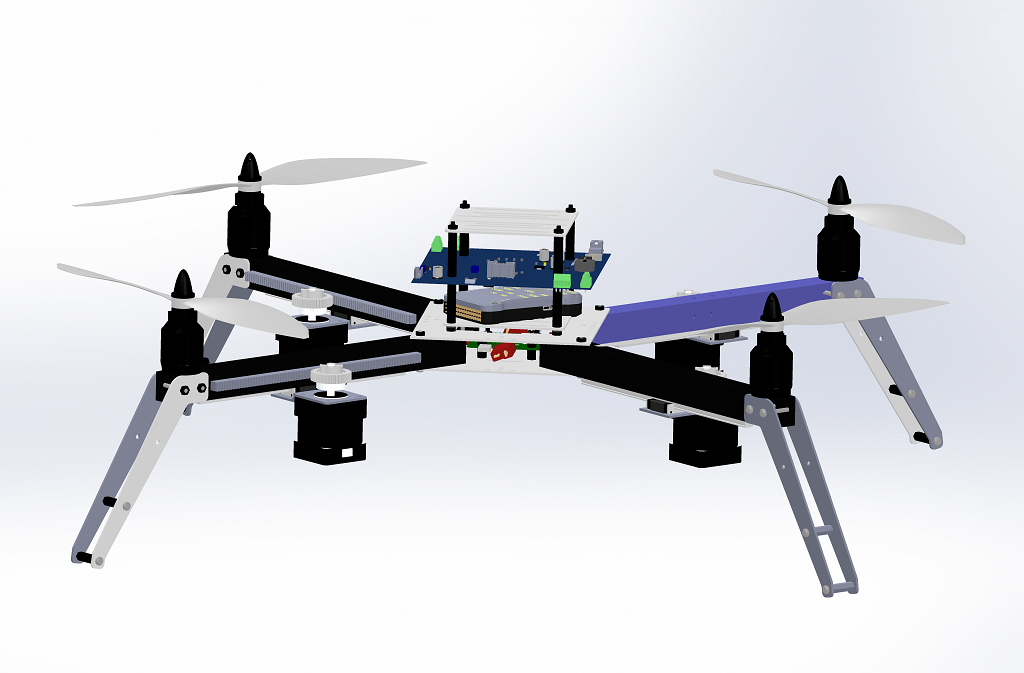
\includegraphics[width=0.9\textwidth]{figures/arducopter_with_PCB.png}
	\caption{3D model modificirane letjelice \textit{ArduCopter}}
	\label{Slika:3D_drone_final}
\end{figure}

\subsection{Letjelica  \textit{ArduCopter}}

Osnova konstrukcije letjelice s pomičnim masama je multirotorska letjelica  \textit{ArduCopter}, prikazano Slikom \ref{fig:3D_drone_original}.  \textit{ArduCopter} je laboratorijska letjelica pogonjena s 4 \textit{beskolektorska DC} motora. Klasičnim konceptom upravljanja, brzom promjenom brzina vrnje motora, ostvaruju se zadani kutevi i kutne brzine letjelice. Letjelica ima modularan dizajn, što omogućava jednostavne nadogradnje, poput različitih upravljačkih uređaja, senzora i aktuatora. Sva proširenja letjelice dodaju se jedno iznad drugoga na već predviđene položaje iznad razine krakova u centru letjelice. Zbog svega navedenog,  \textit{ArduCopter} je odabran kao osnovna platforma za izradu multirotorske letjelice s pomičnim masama.

\medskip

Postojeća mehanička konstrukcija letjelice  \textit{ArduCopter} se u potpunosti koristi, a obuhvaća: 
\begin{center}
	\begin{itemize}
		\item Tijelo letjelice uključujući razvodnu ploču za napajanje iz baterije i prihvat slojeva za proširenje
		\item 4 aluminijska kraka
		\item 4 plastična zaustavna kraka
		\item 4  \textit{beskolektorska DC} motora s pripadnim \textbf{ESC} pogonima
		\item 4 plastična propelera
	\end{itemize}
\end{center}

\subsubsection*{Modifikacija postojeće letjelice}
Predstavljenu postojeću letjelicu \textit{ARDUCOPTER} potrebno je modificirati na sljedeći način:
\begin{center}
	\begin{itemize}
		\item Dodati 4 pokretne mase, odabrati aktuatore, konstruirati i izraditi mehanizam kretanja mase po kraku letjelice.
		\item Dodati kontroler leta \textit{Pixhawk PX4}, za kompletno upravljanje letjelicom s pokretnim masama
		\item Izraditi elektroničko slopovlje potrebno za pogon masa, realizirati komunikaciju s kontrolerom leta te dodati mogućnosti za daljnja funkcionalna proširenja letjelice.
	\end{itemize}
\end{center}


\begin{figure}[H]
	\centering
	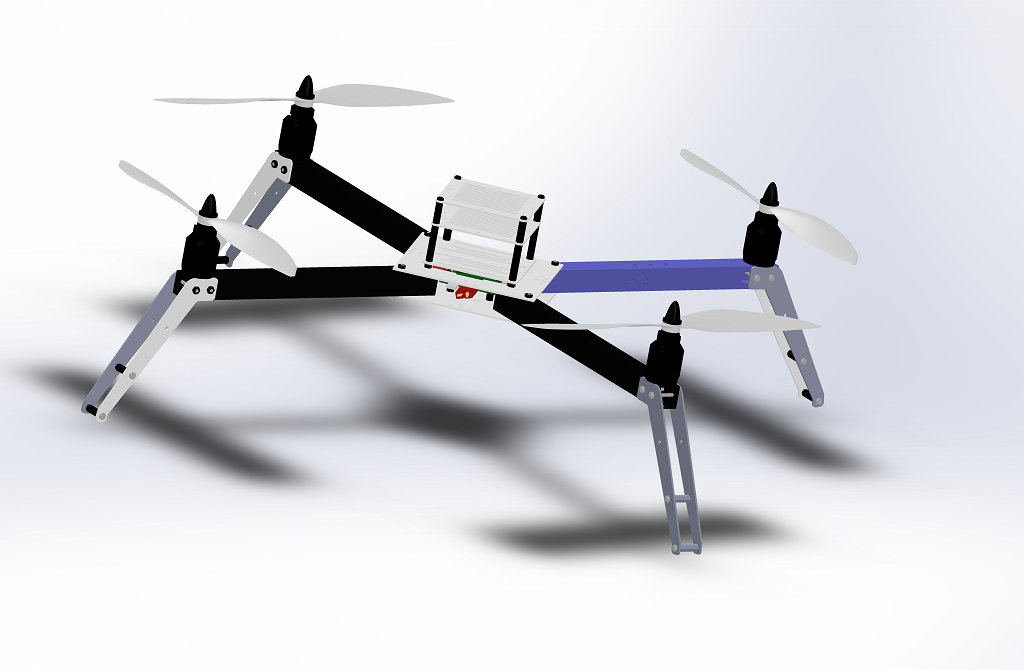
\includegraphics[width=0.9\textwidth]{figures/arducopter_original.png}
	\caption{3D model postojeće letjelice \textit{ArduCopter}}
	\label{fig:3D_drone_original}
\end{figure}

\subsection{Klizni mehanizam pokretne mase}

Budući da se novi koncept upravljanja letjelice zasniva na promjeni centra mase, koje je realizirano pomičnim masama na krakovima, potrebno je izraditi mehanizam kretanja pokretne mase po kraku letjelice. Kretanje pomične mase je linijsko, a mehanizam kretanja mora biti realiziran s minimalnim trenjem. Kretanje pokretne mase ostvareno je električnim aktuatorom.

\subsubsection{Aktuator}
Zadaća je aktuatora pokretne mase gibanje mase po kraku letjelice, čime se ostvaruje promjena centra mase letjelice. Kako bi ukupna masa letjelice bila manja, sam aktuator na svakom kraku se koristi kao pokretna masa. Za aktuator je odabran koračni motor \textit{NEMA 14}, prikazan slikom \ref{fig:stepper_motor}. Specifikacije koračnog motora su prikazane tablicom \ref{tab:specifikacija_steppera}.

\begin{figure}[H]
	\centering
	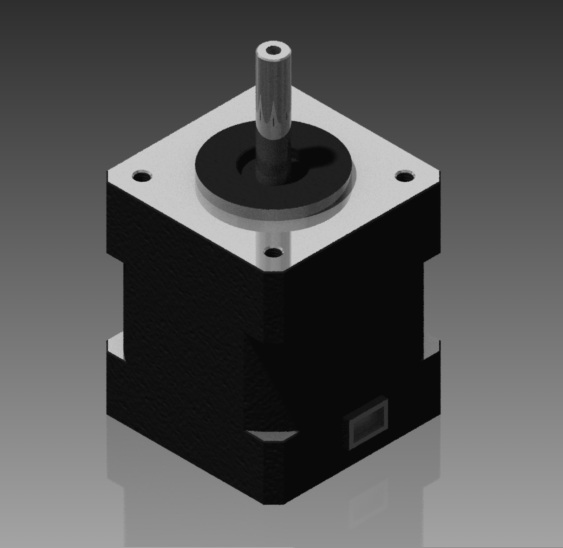
\includegraphics[width=0.3\textwidth]{figures/StepperMotor.jpg}
	\caption{Koračni motor}
	\label{fig:stepper_motor}
\end{figure}


\begin{table}[H]
	\centering
	\caption{Specifikacije koračnog motora }
	\label{tab:specifikacija_steppera}
	\begin{tabular}{|l|c|}
		\hline
		\textbf{Proizvođač} &PROIZVOĐAČ \\ \hline 
		\textbf{Model} & NEMA 14  \\ \hline 
		\textbf{Veličina} & 35mm x 35mm x 36mm, neuključujući osovinu  \\ \hline 
		\textbf{Masa} & 180 g  \\ \hline 
		\textbf{Promjer osovine} & 5 mm \\ \hline 
		\textbf{Broj koraka po okretu} & 200 \\ \hline 
		\textbf{Broj faza} & 2 \\ \hline 
		\textbf{Current rating} & 1A po fazi \\ \hline 
		\textbf{Moment zadržavanja} & 1.4 $kg/cm$ \\ \hline 
		\textbf{Moment inercije rotora} & 14 $g/cm^2$ \\ \hline 
	\end{tabular}
\end{table}

Koračni motor odabran je zato jer pruža mogućnost korištenja upravljanja pozicijom motora u otvorenoj petlji. Točnije, pravilnim upravljanjem i brojanjem koraka koje je motor napravio, moguće je u svakom trenutku znati u kojem položaju se motor nalazi te samim time i na kojoj poziciji se nalazi pokretna masa. Ako bi se koristio neki drugi tip motora, bilo bi potrebno dodati senzore poput enkodera kako bi se moglo pratiti kretanje i položaj mase na kraku.




\subsubsection{Kretanje po kraku letjelice}

Kretanje mase po kraku je linijsko. Kako bi kretanje mase imalo minimalno trenje, odabran je klizni mehanizam prikazan slikom \ref{fig:klizni_mehanizam}. Klizni mehanizam montiran je s doljnje strane kraka, a za aluminijsku kvadratnu cijev pričvršćen je s dva vijka. Klizni mehanizam se sastoji od vodilice i kolica. Na kolicima se nalazi klizni mehanizam koji se sastoji od sitnih kuglica koje omogućavaju klizno gibanje s malim trenjem. Na kolica kliznog mehanizma montirano je posebno konstruiran prihvat koračnog motora(slika \ref{fig:stepper_bracket}), kojim se koračni motor učvršćuje na klizni mehanizam.


\begin{figure}[H]
\centering
\begin{minipage}{.5\textwidth}
  \centering
  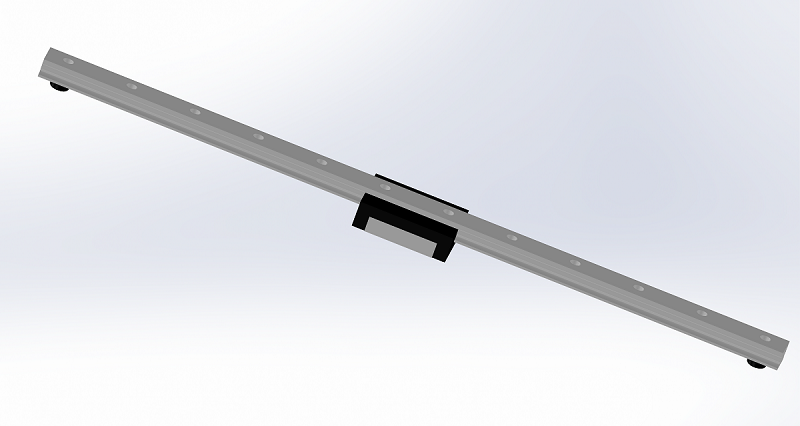
\includegraphics[width=.9\linewidth]{figures/linear_guide_7mm.png}
  \captionof{figure}{Klizni mehanizam}
  \label{fig:klizni_mehanizam}
\end{minipage}%
\begin{minipage}{.5\textwidth}
  \centering
  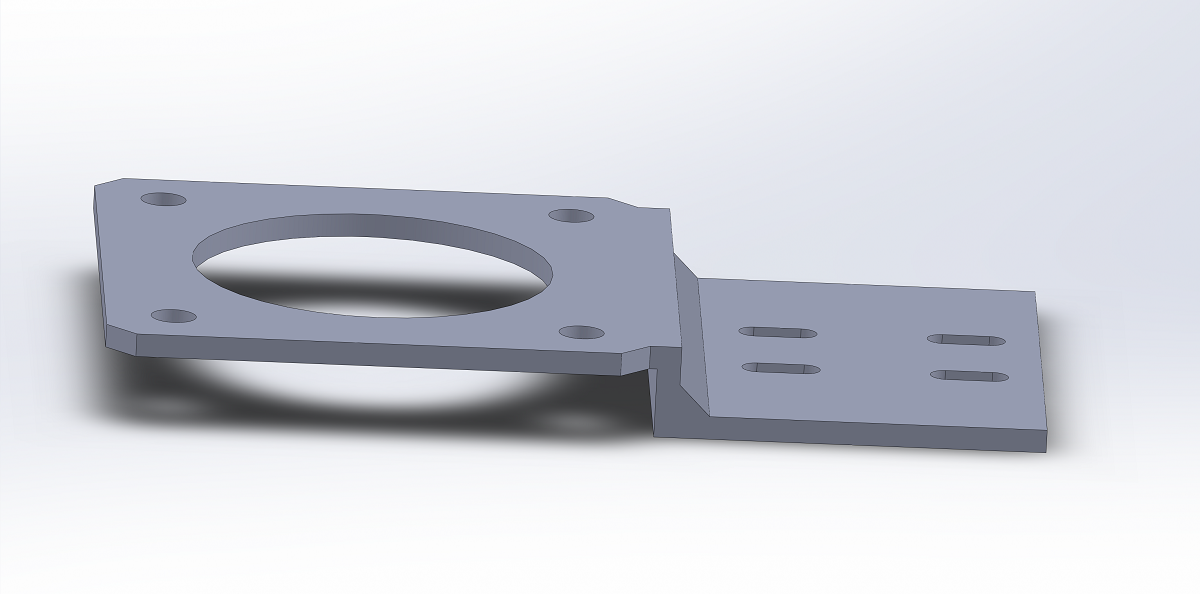
\includegraphics[width=.9\linewidth]{figures/stepper_bracket.png}
  \captionof{figure}{Prihvat koračnog motora}
  \label{fig:stepper_bracket}
\end{minipage}
\end{figure}

Rotacija koračnih motora se prenosi na linijsko gibanje po kraku pomoću zupčastog prijenosa. Zupčasti prijenos je dizajniran tako da jedan puni okret koračnog motora pokriva cijeli potrebni raspon linijskog gibanje na kraku. 
Zupčasta letva(slika \ref{fig:gear_rack}) je zaljepljena na bočnu stranu aluminijske kvadratne cijevi pomoću dvokomponentnog ljepila. Zupčanik(slika \ref{fig:gear_gear}) se montira na adapter osovine koračnog motora pomoću 4 vijka. 



\begin{figure}[H]
\centering
\begin{subfigure}{.5\textwidth}
  \centering
  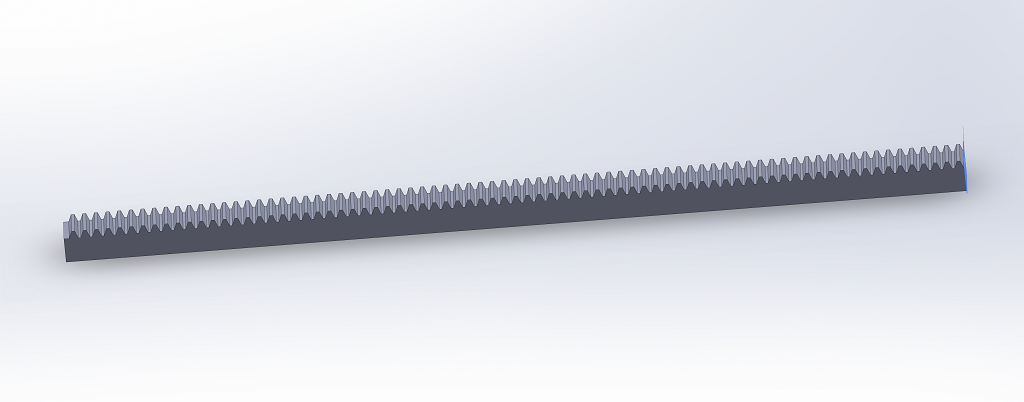
\includegraphics[width=.9\linewidth]{figures/gear_rack_6mm.png}
  \caption{Zupčasta letva}
  \label{fig:gear_rack}
\end{subfigure}%
\begin{subfigure}{.5\textwidth}
  \centering
  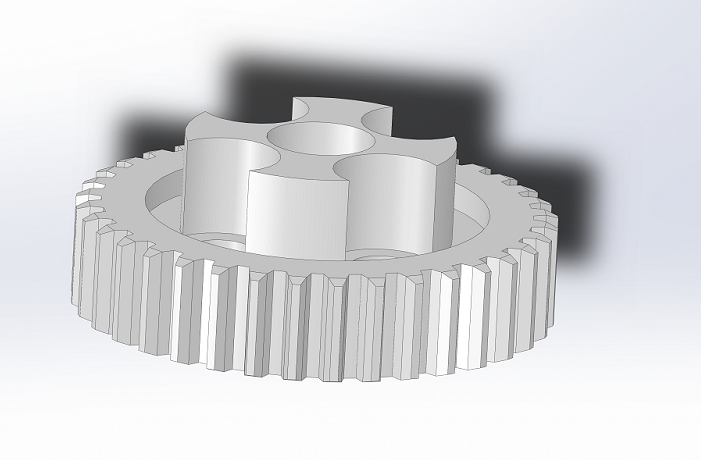
\includegraphics[width=.9\linewidth]{figures/gear_25_07.png}
  \caption{Zupčanik}
  \label{fig:gear_gear}
\end{subfigure}

\caption{Prikaz elemenata zupčastog prijenosa}
\label{fig:gear}
\end{figure}


\subsubsection{Izrada i montaža}

Za dizajniranje mehaničke konstrukcije korišten je CAD alat, koji omogućava 3D modeliranje svih dijelova od kojih je izrađena letjelica. Nakon dizajniranja svakog pojedinog dijela, prelazi se na spajanje dijelova u veće cjeline. Prednost 3D modeliranja je trenutni pregled izgleda konstrukcije, kao i mogućnost izvoza svakog pojedinog dijela u neki od standardnih formata. 

U izradi nekih dijelova konstrukcije korištena je tehnologija 3D printanja. 3D printanje jednostavno je i efikasno rješenje u izradi prototipa. Nakon izrade 3D modela u nekom od CAD alata, radi se priprema pojedinog elementa za izradu. Priprema uključuje učitavanje elementa u poseban softver proizvođača 3D printera. Nakon postavljanja svih parametara izrade poput preciznosti, ispunjenosti i dr. slijedi izvoz podataka u standardan \textit{gcode} format koji koristi 3D printer. Nakon toga slijedi izrada koja je u potpunosti automatizirana.

Dodatno, za montažu kliznih mehanizama na aluminijske kvadratne cijevi potrebno je precizno izbušiti rupe, kroz koje će se pomoću vijka pričvrstiti klizni mehanizam. Zbog toga je korišten CNC stroj.

Nakon pripreme svih dijelova, slijedi montaža. Slikom \ref{fig:arm_assembly} prikazan je konačni 3D model pokretne mase na kraku letjelice.


\begin{figure}[H]
\centering
\begin{subfigure}{.5\textwidth}
  \centering
  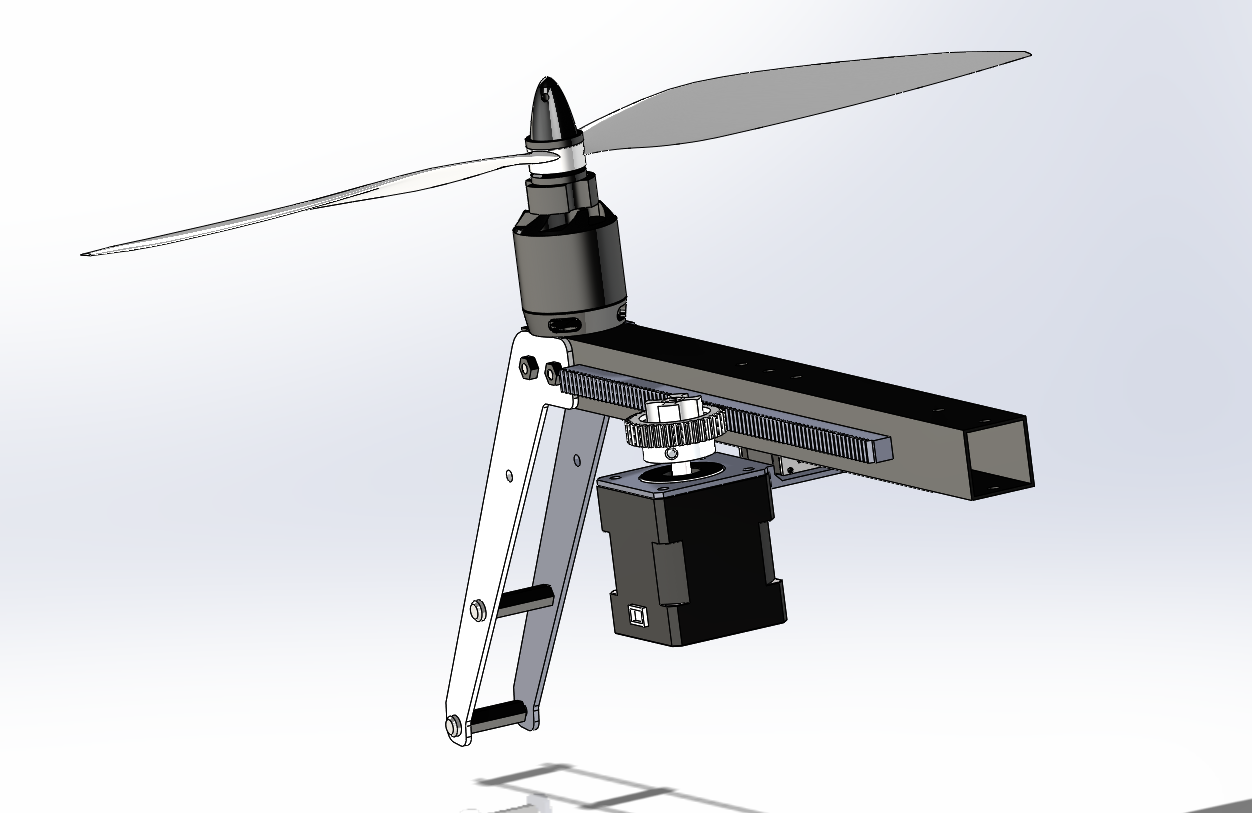
\includegraphics[width=.9\linewidth]{figures/arm_assembly1.png}
  \caption{Pogled 1}
  \label{fig:sub1}
\end{subfigure}%
\begin{subfigure}{.5\textwidth}
  \centering
  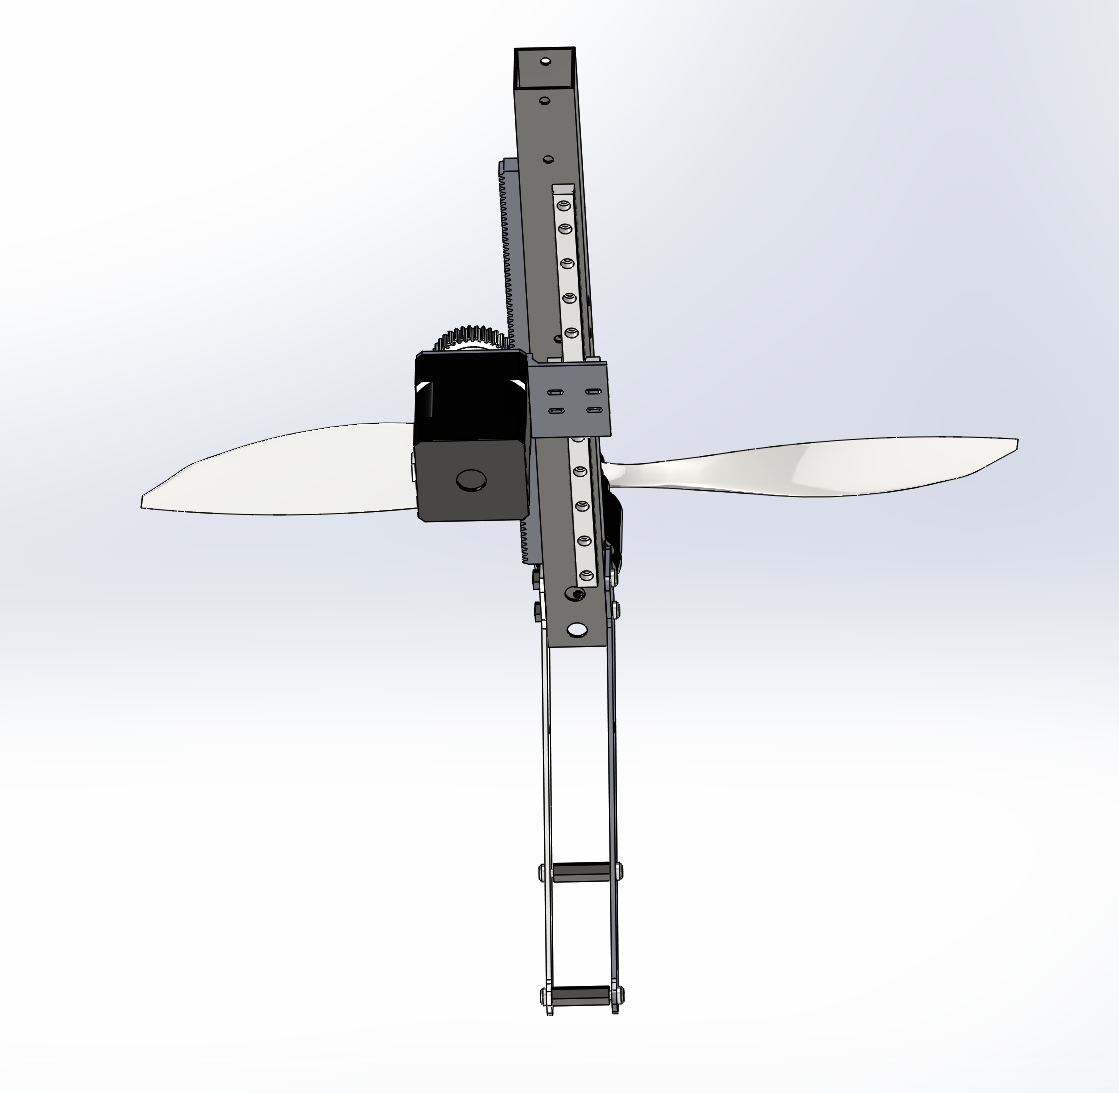
\includegraphics[width=.9\linewidth]{figures/arm_assembly2.png}
  \caption{Pogled 2}
  \label{fig:sub2}
\end{subfigure}
\caption{Prikaz 3D modela jednog kraka letjelice s pomičnom masom}
\label{fig:arm_assembly}
\end{figure}


Nakon montaže svih dijelova, modificirana letjelica \textit{ArduCopter} postavljena je na stalak, s omogućenim jednim stupnjem slobode. Konačni izgled letjelice postavljene na stalak prikazan je Slikom \ref{fig:arm_assembly_Real}.

\begin{figure}[H]
	\centering
	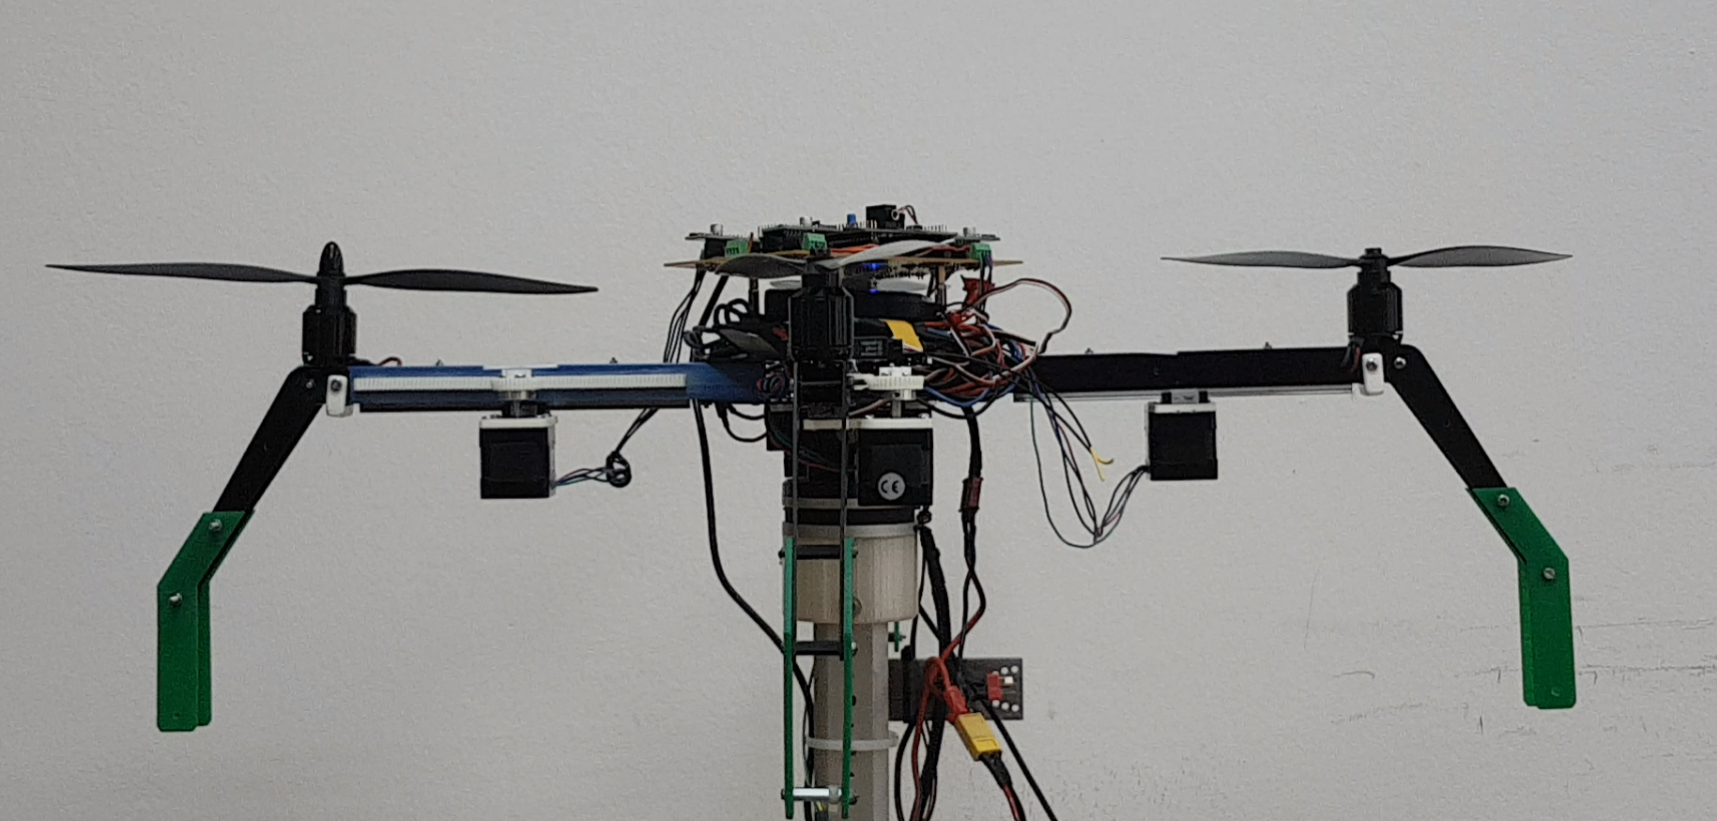
\includegraphics[width=0.9\textwidth]{figures/letjelica.png}
	\caption{Prikaz laboratorijskog modela letjelice s pomičnom masom}
	\label{fig:arm_assembly_Real}
\end{figure}



\subsection{Horizontalna montaža sastavnih dijelova letjelice}
Modularni dizajn letjelice \textit{ArduCopter} omogućava jednostavno proširenje letjelice. Iznad ravnine krakova moguće je dodavati razne slojeve. Slojevi su razmaknuti distancerima s navojem M3. 

\subsubsection{Sloj kontrolera leta}

Kontroler leta \textit{Pixhawk} se koristi za cjelokupno upravljanje letjelicom. U samom kontroleru su ugrađeni svi potrebni senzori za let, poput žiroskopa, akcelerometra i dr. Kontroler leta potrebno je postaviti što bliže osima rotacije letjelice. U ovom slučaju kontroler je postavljen neposredno iznad ravnine krakova. Položaj kontrolera leta prikazan je slikom \ref{fig:slot_pixhawk}.

\begin{figure}[H]
	\centering
	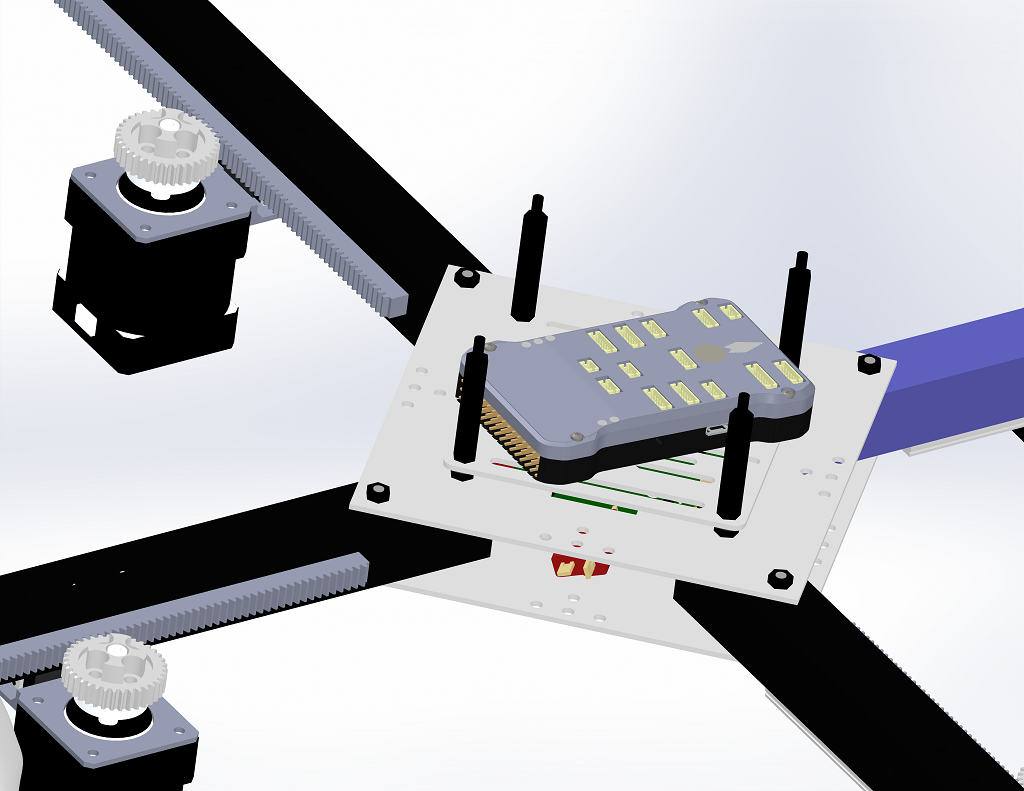
\includegraphics[width=0.7\textwidth]{figures/arducopter_slot_pixhawk.png}
	\caption{Sloj kontrolera leta}
	\label{fig:slot_pixhawk}
\end{figure}


\subsubsection{Sloj upravljačkog sklopovlja}

Iznad kontolera leta postavljeno je posebno izrađeno elektroničko slopovlje za upravljanje koračnim motorima. Dimenzija tiskane pločice jednaka je dimenziji bazne ploče koja se nalazi u ravnini krakova. Pločica je 
razmaknuta od kontrolera leta pomoću distancera. Pozicioniranje upravljačkog sklopovlja prikazano je Slikom \ref{fig:slot_pcb}.


\begin{figure}[H]
	\centering
	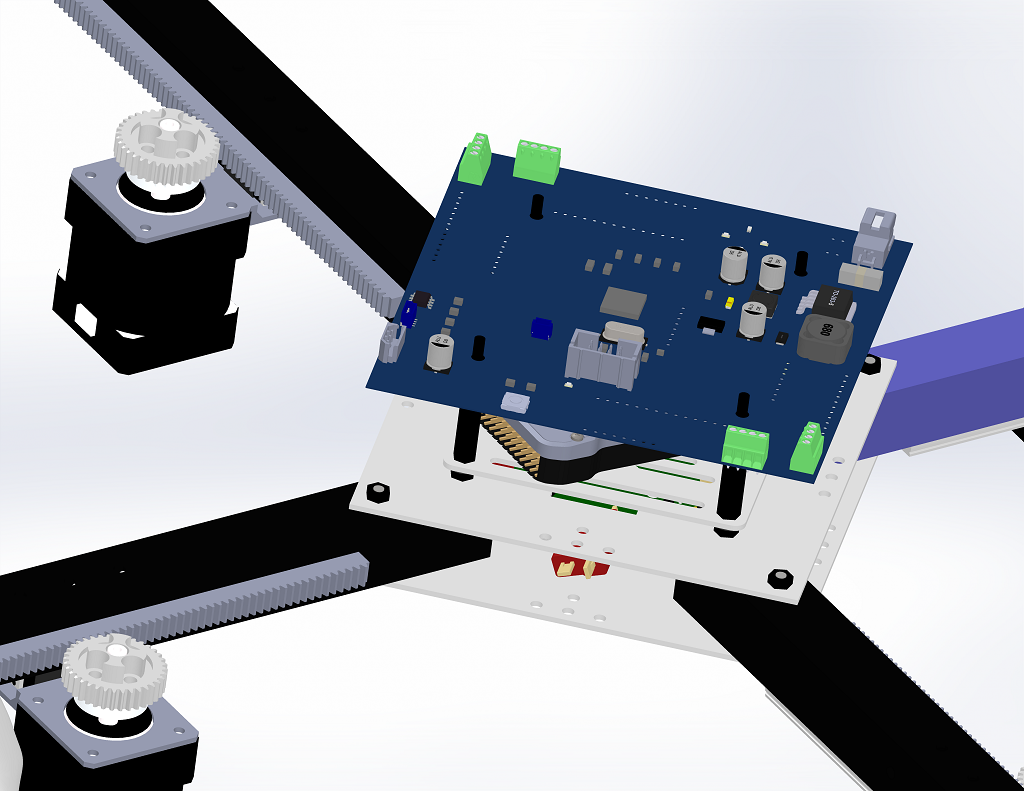
\includegraphics[width=0.7\textwidth]{figures/arducopter_slot_pcb.png}
	\caption{Sloj upravljačkog sklopovlja}
	\label{fig:slot_pcb}
\end{figure}

\subsubsection{Sloj za proširenje}
Iznad upravljačkog sklopovlja, nalazi se sloj za daljnja proširenja. Daljnja proširenja predstavlja dodavanje raznih senzora za pozicioniranje u prostoru i sl. 

\begin{figure}[H]
	\centering
	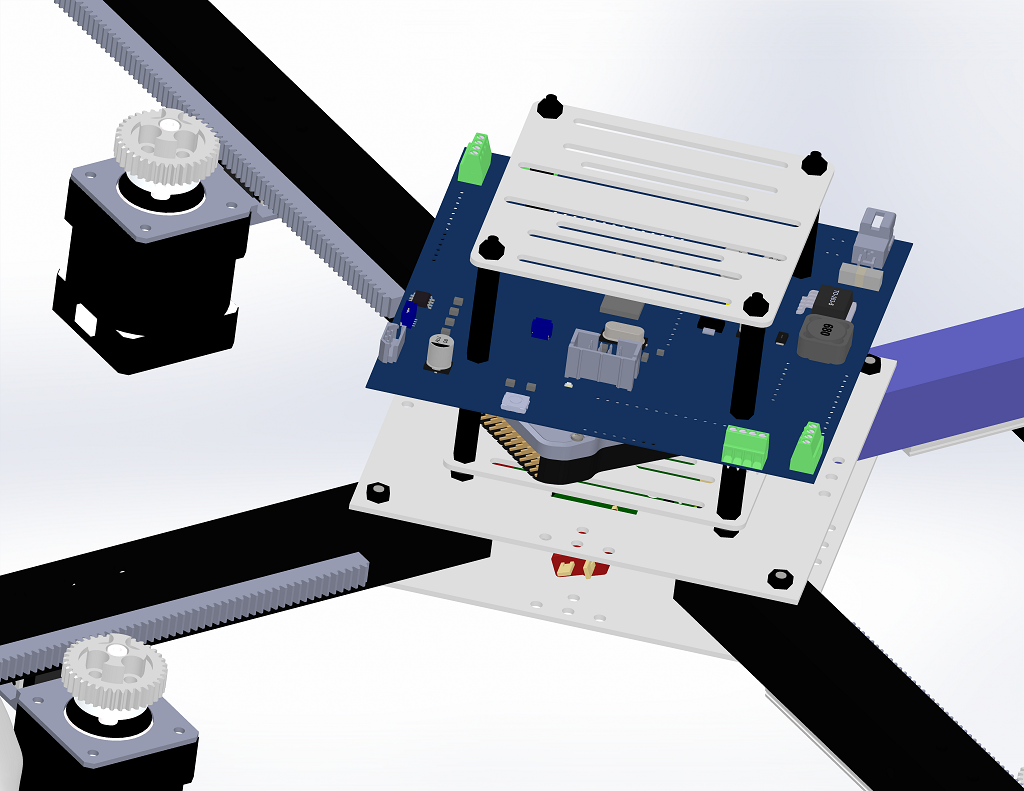
\includegraphics[width=0.7\textwidth]{figures/arducopter_slot_top.png}
	\caption{Sloj za proširenje}
	\label{fig:slot_top}
\end{figure}

\subsection{Prikaz rezalizacije mehaničke konstrukcije}
OVDJE STAVITI FOTOGRAFIJE STVARNE LETJELICE


\end{document}

\newpage
\section{Elektroničko sklopovlje}
%%%%%%%%%%%%%%%%%%%%%%%%%%%%%%%%

\documentclass[11pt,a4paper]{article}
\usepackage{times}
\usepackage[utf8]{inputenc}
\usepackage[croatian]{babel}
\usepackage[T1]{fontenc} % Latin Modern

%%%%%%%%%%%%%%%%%%%%%%%%%%%%%%%%


%%%%%%%%%%%%%%%%%%%%%%%%%%%%%%%%
%%%%%%%%  MATEMATICKI PAKETI %%%%%%%%%%%
%%%%%%%%%%%%%%%%%%%%%%%%%%%%%%%%

\usepackage{amsmath}
\usepackage{amsfonts}
\usepackage{amssymb}
\usepackage{esvect}

%%%%%%%%%%%%%%%%%%%%%%%%%%%%%%%%

%%%%%%%%%%%%%%%%%%%%%%%%%%%%%%%%
%%%%%%%%%% PAKETI ZA SLIKE  %%%%%%%%%%%%
%%%%%%%%%%%%%%%%%%%%%%%%%%%%%%%%

\usepackage{graphicx}
\usepackage{float}
\usepackage[hidelinks]{hyperref}
\usepackage{caption}
\usepackage{subcaption}
\usepackage{booktabs}

%%%%%%%%%%%%%%%%%%%%%%%%%%%%%%%%

%%%%%%%%%%%%%%%%%%%%%%%%%%%%%%%%
%%%%%%%%%    PRORED 1.5   %%%%%%%%%%%%%%
%%%%%%%%%%%%%%%%%%%%%%%%%%%%%%%%

\renewcommand{\baselinestretch}{1.5}

%%%%%%%%%%%%%%%%%%%%%%%%%%%%%%%%


%%%%%%%%%%%%%%%%%%%%%%%%%%%%%%%%
%%%%%%%%%% TABLICA - ANTUN %%%%%%%%%%%%
%%%%%%%%%%%%%%%%%%%%%%%%%%%%%%%%

\usepackage{array}
\usepackage{multirow}
\newcolumntype{C}[1]{>{\centering\let\newline\\\arraybackslash\hspace{0pt}}m{#1}}
\newcolumntype{L}[1]{>{\raggedright\let\newline\\\arraybackslash\hspace{0pt}}m{#1}}
\newcolumntype{R}[1]{>{\raggedleft\let\newline\\\arraybackslash\hspace{0pt}}m{#1}}
\usepackage{ctable}

%%%%%%%%%%%%%%%%%%%%%%%%%%%%%%%%

%%%%%%%%%%%%%%%%%%%%%%%%%%%%%%%%
%%%%%%%%%% TABLICA - MARTINA %%%%%%%%%%%
%%%%%%%%%%%%%%%%%%%%%%%%%%%%%%%%

\makeatletter
\renewcommand*\env@matrix[1][\arraystretch]{%
  \edef\arraystretch{#1}%
  \hskip -\arraycolsep
  \let\@ifnextchar\new@ifnextchar
  \array{*\c@MaxMatrixCols c}}
\makeatother



%%%% LATEX KOD ZA KORISTENJE TABLICE %%%%
%%% PRIMJER %%%

%\setlength\extrarowheight{1pt}
%\begin{table}[h]
%\centering
%\caption{Tablica s prikazom }
%\label{prva}
%\begin{tabular}{|l|c|}
%\hline
%\textbf{txt} &  \\ \hline 
%txt & txt    \\ 
%txt & txt   \\ \hline
%txt & txt    \\ \hline
%\end{tabular}
%\end{table}

%%%%%%%%%%%%%%%%%%%%%%%%%%%%%%%%


%%%%%%%%%%%%%%%%%%%%%%%%%%%%%%%%
%%%%%%% DIO ZA UNOS ISJECAKA KODA %%%%%%%%
%%%%%%%%%%%%%%%%%%%%%%%%%%%%%%%%

\usepackage{listings}
\usepackage{color}
 
\definecolor{codegreen}{rgb}{0,0.6,0}
\definecolor{codegray}{rgb}{0.5,0.5,0.5}
\definecolor{codepurple}{rgb}{0.58,0,0.82}
 
\lstdefinestyle{mystyle}{   
    commentstyle=\color{codegreen},
    keywordstyle=\color{blue},
    numberstyle=\tiny\color{codegray},
    stringstyle=\color{codepurple},
    basicstyle=\footnotesize,
    breakatwhitespace=false,         
    breaklines=true,                 
    captionpos=b,                    
    keepspaces=true,                 
    numbers=left,                    
    numbersep=5pt,                  
    showspaces=false,                
    showstringspaces=false,
    showtabs=false,                  
    tabsize=1
}
 
\lstset{style=mystyle}

%\lstinputlisting[language=Matlab, firstline=1, lastline=4, numbers=left, frame=single, label={lst:prvi}, caption={Diskretizacija sustava korištenjem Matlaba}, captionpos=b]{peti.m} 

%%%%%%%%%%%%%%%%%%%%%%%%%%%%%%%%


%----------------------------
% za uredjenje stranice
\usepackage[left=2.5cm,right=2.5cm,top=2.5cm,bottom=2.5cm]{geometry}
\usepackage{fancyhdr}
\pagestyle{fancy} 
\lhead{\leftmark}
\rhead{\rightmark}
\usepackage{titlesec} %za točku iza broja sectiona
\titleformat{\section}{\huge\bfseries}{\thetitle.\quad}{0em}{}
\titleformat{\subsection}{\LARGE\bfseries}{\thetitle.\quad}{0em}{}
\titleformat{\subsubsection}{\Large\bfseries}{\thetitle.\quad}{0em}{}
\titleformat{\paragraph}
{\normalfont\large\bfseries}{\thetitle.\quad}{1em}{}
\titlespacing*{\paragraph}
{0pt}{3.25ex plus 1ex minus .2ex}{1.5ex plus .2ex}
\setcounter{secnumdepth}{5}

\usepackage{indentfirst} %uvlacenje prvog paragrafa
% primjer pozivanja sectiona
% \section*{UVOD} \pdfbookmark{UVOD}{section:UVOD}

\usepackage{tocloft}
\usepackage{import}
\usepackage{standalone}
\graphicspath{{Uvod/}, {Ciljevi/}, {Materijal/}, {Rasprava/}, {Rezultati/}} 

\hypersetup{
  colorlinks   = true, %Colours links instead of ugly boxes
  urlcolor     = black, %Colour for external hyperlinks
  linkcolor    = black, %Colour of internal links
  citecolor   = blue %Colour of citations
}

\usepackage{subcaption}
\usepackage{lscape}
\begin{document}

POGLAVLJE NAZVATI ELEKTRONIČKO SLOPOVLJE

U ovom poglavlju je predstavljen dizajn i izrada elektroničkog sklopovlja potrebnog za upravljanje multirotorskom letjelicom s pomičnim masama. Elektroničko sklopovlje je ciljano dizajnirano za upravljanje koračnim motorima koji u ovom slučaju predstavljaju pokretne mase. Također, kao pripremu za daljnja proširenja, dodana su standarna sučelja za komunikaciju i akuatore koje u ovom trenutku očekujemo da bi se mogli primjeniti na ovoj letjelici. Elektroničko sklopovlje je zasnovano na mikrokontroleru STM32 tipa F4. Dodatno, na elektroničkom sklopovlju trebaju postojati izvodi napajanja standardnih iznosa $3.3 V$ i $5 V$. Sklopovlje se napaja iz baterije nazivnog napona $12 V$. 

Dizajn elektroničkog sklopovlja izrađen je u CAD alatu Altium. Altium predstavlja standardni CAD alat za izradu elektroničkog sklopovlja. U okviru ovog alata, definiraju se sve potrebne elektroničke komponente, s pripadnim fizičkim rasporedom veza i mogućnošću dodavanja 3D modela svake pojedine komponente. Prvo se pristupa projektiranju sklopovlja na shematskoj razini. U ovom koraku definiraju se sve sheme, određuju se komponente koje je kasnije potrebno kupiti sa svim pripadnim podacima. Nakon završetka prve faze projektiranja, slijedi fizički raspored komponenata na tiskanu pločicu i povezivanje svih električnih veza. U obije faze projekiranja, softver omogućava kontrolu prema zadanim postavkama te na taj način upozorava korisnika ukoliko je došlo do kršenja zadanih pravila, poput kratkih spojeva, prebliskih električnih vodova i slično.

Funkcionalnost elektroničkog sklopovlja i programske potpore je provjerena izradom prototipa. Prototip je realiziran perforiranom pločicom, na koju su postavljene i povezane sve bitne komponente, prvenstveno pogoni koračnih motora. Upravljanje pogonima koračnih motora omogućeno je razvojnom pločicom STM Discovery, koja je bazirana na STM32 mikrokontroleru tipa F4, koji je korišten i u konačnom posebno prilagođenom sklopovlju.

TU DODATI 3D MODEL SKLOPOVLJA

\begin{figure}[H]
	\centering
	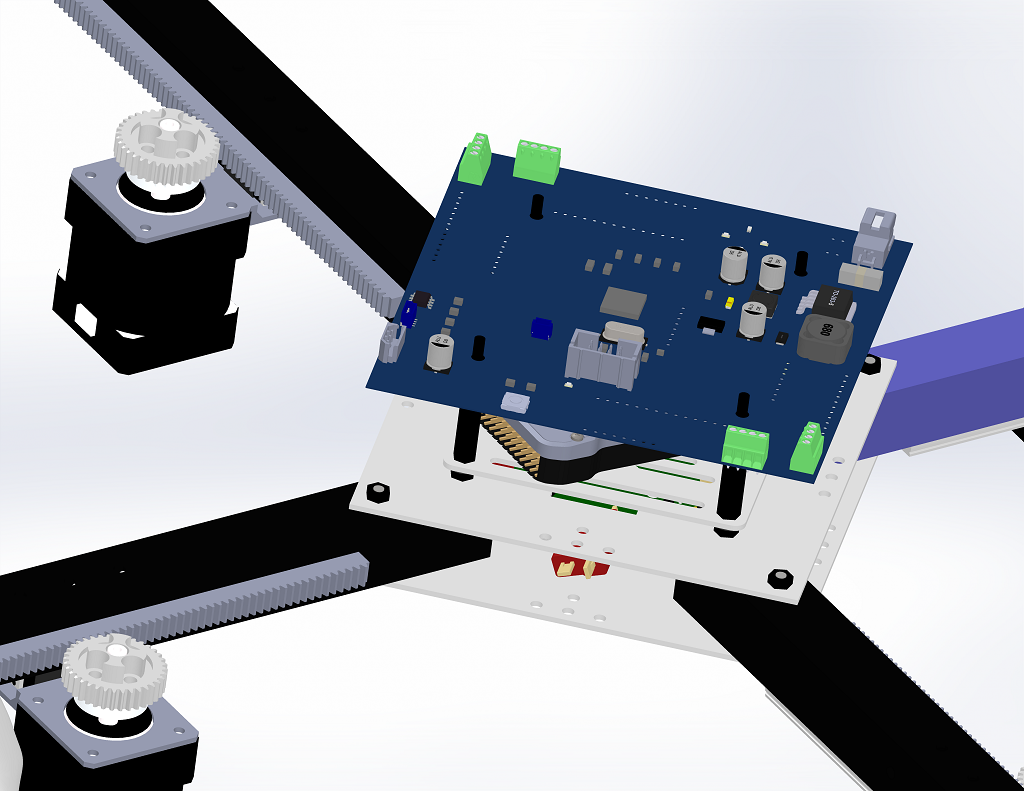
\includegraphics[width=0.9\textwidth]{figures/arducopter_slot_pcb.png}
	\caption{3D model elektroničkog sklopovlja}
	\label{Slika:3D_PCB}
\end{figure}

\subsection{Sastavni dijelovi elektroničkog slopovlja}

\subsubsection{Napajanje}
Napajanje elektroničkog sklopovlja osigurano je baterijom nazivnog napona 12 V. Na ulazu napajanja dodan je osigurač iznosa 10A. Iznos osigurača je projektiran prema maksimalnim iznosima struja koje se mogu ostvariti na koračnim motorima. Dodatno, značajniji potrošači na ovom sklopovlju su Dynamixel motori, čije je sučelje dodano za daljnja proširenja funkcionalnosti letjelice.
U sklopu modula napajanja, potrebno je osigurati stabilne iznose napona 3.3 V i 5V. Prva razina spuštanja ulaznog napona je osigurana 5V regulatorom napona, switching tipa. Specifikacije regulatora su prikazane tablicom \ref{tab:specifikacija_5V}.


\begin{table}[H]
	\centering
	\caption{Specifikacije 5V regulatora napona: }
	\label{tab:specifikacija_5V}
	\begin{tabular}{|l|c|}
		\hline
		\textbf{Proizvođač} & Texas instuments  \\ \hline 
		\textbf{Model} &  LM2592HVS-5.0  \\ \hline 
		\textbf{Tip} &  Buck(Step Down) Switching Regulator  \\ \hline 
		\textbf{Minimalni ulazni napon} & 4.5 V \\ \hline 
		\textbf{Maksimalni ulazni napon} & 60 V \\ \hline 
		\textbf{Izlazni napon} & 5 V \\ \hline 
		\textbf{Izlazna struja} & 2 A \\ \hline 
		\textbf{Frekvencija rada} & 150 kHz \\ \hline 
		\textbf{Maksimalna radna temperatura} & $125 \deg C$ \\ \hline 
	\end{tabular}
\end{table}

Nadalje, napon iznosa 3.3 V osiguran je snižavanjem 5V napona iz prethodno opisanog regulatora. U ovom slučaju korišten je linearni regulator. Korištenje ovog tipa regulatora je moguće, budući da je snaga potrošača spojenih na napajanje 3.3 V daleko manja od maksimalnog iznosa struje koju daje 5 V regulator. Specifikacije 3.3 V regulatora prikazane su tablicom \ref{tab:specifikacija_3V3}

\begin{table}[H]
	\centering
	\caption{Specifikacije 3.3V regulatora napona: }
	\label{tab:specifikacija_3V3}
	\begin{tabular}{|l|c|}
		\hline
		\textbf{Proizvođač} & ST Microelectronics \\ \hline 
		\textbf{Model} &  LD1117S33TR \\ \hline 
		\textbf{Tip} &  Fixed LDO Voltage Regulator  \\ \hline 
		\textbf{Minimalni ulazni napon} & 4.75 V \\ \hline 
		\textbf{Maksimalni ulazni napon} & 15 V \\ \hline 
		\textbf{Izlazni napon} & 3.3 V \\ \hline 
		\textbf{Izlazna struja} & 800 mA \\ \hline 
		\textbf{Maksimalna radna temperatura} & $125 \deg C$ \\ \hline 
	\end{tabular}
\end{table}

U sklopu modula napajanja, potrebno je osigurati i napajanje koračnih motora te napajanje Dynamixel motora. U ovom slučaju, koristi se ulazni napon, međutim dodani su jumperi, kako bi na jednostavan način bilo moguće odspojiti navedene potrošače u fazi programiranja elektroničkog sklopovlja.

\subsubsection{Mikrokontroler}
 Elektroničko sklopovlje je bazirano na mikrokontroleru STM32, serije F4. Jezgra mikrokontrolera je zasnovana na jezgri ARM(R) Cortex$^{TM}$-M4, 32-bit, RISC arhitekture. Na mikrokontroler su povezane sve komponente kojima je potrebno upravljati i s kojih je potrebno očitavati stanja. Specifikacije mikrokontrolera su prikazane tablicom \ref{tab:specifikacija_MCU}.

\begin{table}[H]
	\centering
	\caption{Specifikacije STM mikrokontrolera: }
	\label{tab:specifikacija_MCU}
	\begin{tabular}{|l|c|}
		\hline
		\textbf{Proizvođač} & ST Microelectronics \\ \hline 
		\textbf{Model} &  STM32F405RGT6V \\ \hline 
		\textbf{Jezgra} &  ARM(R) Cortex$^{TM}$-M4, 32-bit, RISC  \\ \hline 
		\textbf{CPU brzina} & 168 MHz \\ \hline 
		\textbf{Veličina RAM memorije} & 192 KB \\ \hline 
		\textbf{Broj pinova} & 64 \\ \hline 
		\textbf{Broj I/O jedinica} & 51 \\ \hline 
		\textbf{Ugrađena sučelja} & CAN, I2C, SPI, UART, USART, USB\\ \hline 
		\textbf{Minimalni napon napajanja} & 1.8 V\\ \hline 
		\textbf{Maksimalni napon napajanja} & 3.6 V\\ \hline 
	\end{tabular}
\end{table}

Napajanje mikrokontrolera je osigurano reguliranim naponom iznosa 3.3 V. Dodatno stabiliziranje napona je osigurano dodavanjem kondenzatora različitih iznosa. Dodatni kondenzatori su smješteni u neposrednoj blizini mikrokontrolera na tiskanoj pločici.
Za izvor takta mikrokontrolera korišten je kristalni oscilator nazivne frekvencije 8 Mhz.

\subsubsection{LED indikatori}
Prilikom izrade prototipa elektroničkog sklopovlja utvrđena je potreba postojanja LED indikatora. LED indikatori se koriste u svrhu provjere ispravnosti rada programske potpore. U ovom slučaju, dodane su 4 LED diode različitih boja. LED diode su spojene na mikorokontroler, a za izvor napajanja se koristi regulirani napon iznosa 5V. Upravljanje LED diodama je ostvareno mikrokontrolerom i bipolarnim NPN tranzistorom. Struja koja protječe LED diodom prilikom visoke razine upravljačkog signala iz mikrokontrolera je ograničena dodavanjem otpornika iznosa 500 V. 


\subsubsection{Pogon koračnih motora}

Pogon koračnih motora ostvaren je gotovim sklopom A4988. Navedeni sklop ima sadržano upravljanje naponima i strujama svake faze koračnog motora. Pogonski sklop predstavlja međusklop između koračnog motora i mikroprocesora. Mikroprocesor postavljanjem logičkih razina na predviđene pinove upravlja smjerom vrtnje i rezolucijom koraka. Kretanje motora je izvodi generiranjem impulsnog signala. Generiranje impulsnog signala je ostvareno prikladnom programskom potporom mikrokontrolera. Specifikacije sklopa A4988 prikazane su tablicom \ref{tab:specifikacija_stepper_driver}.


\begin{figure}[H]
	\centering
	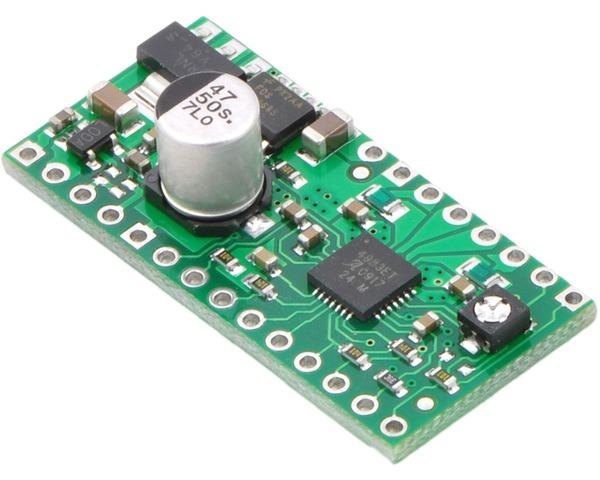
\includegraphics[width=0.4\textwidth]{figures/driver.jpg}
	\caption{Prikaz pogona koračnog motora}
	\label{Slika:stepper_driver}
\end{figure}

Sklop A4988 se napaja izravno s baterije, a napajanje logike je ostvareno korištenjem ugrađenih regulatora napona u samom sklopu. Mikrokontroler upravlja radom pogonskog sklopa pomoću 5 pinova:
\begin{center}
	\begin{itemize}
		\item STP - impulsni signal broja koraka
		\item DIR - smjer vrtnje motora
		\item MS1 - upravljanje rezolucijom koraka
		\item MS2 - upravljanje rezolucijom koraka
		\item MS3 - upravljanje rezolucijom koraka
	\end{itemize}
\end{center}


\begin{table}[H]
	\centering
	\caption{Specifikacije pogona koračnih motora: }
	\label{tab:specifikacija_stepper_driver}
	\begin{tabular}{|l|c|}
		\hline
		\textbf{Proizvođač} & Pololu \\ \hline 
		\textbf{Model} & A4988 \\ \hline 
		\textbf{Veličina} &    \\ \hline 
		\textbf{Masa} & 3.3 g \\ \hline 
		\textbf{Minimalni ulazni napon} & 8 V \\ \hline 
		\textbf{Maksimalni ulazni napon} & 35 V \\ \hline 
		\textbf{Kontinuirana stuja po fazi} & 1 A, bez hladnjaka \\ \hline 
		\textbf{Maksimalna struja po fazi} & 2 A, s hladnjakom \\ \hline 
		\textbf{Minimalni napon logike} & 3 V\\ \hline 
		\textbf{Maksimalni napon logike} & 5.5 V\\ \hline 
		\textbf{Rezolucija mikrokoraka} & puni korak, 1/2, 1/4, 1/8 i 1/16\\ \hline 
		\textbf{Zaštita obrnutog polariteta} & Da\\ \hline 
	\end{tabular}
\end{table}


\subsubsection{Konektori}



\subsubsection{Dynamixel}
\subsubsection{CAN}

\subsection{Tiskana pločica - PCB}


\end{document}

\newpage
\section{Programska struktura}
%%%%%%%%%%%%%%%%%%%%%%%%%%%%%%%%

\documentclass[11pt,a4paper]{article}
\usepackage{times}
\usepackage[utf8]{inputenc}
\usepackage[croatian]{babel}
\usepackage[T1]{fontenc} % Latin Modern

%%%%%%%%%%%%%%%%%%%%%%%%%%%%%%%%


%%%%%%%%%%%%%%%%%%%%%%%%%%%%%%%%
%%%%%%%%  MATEMATICKI PAKETI %%%%%%%%%%%
%%%%%%%%%%%%%%%%%%%%%%%%%%%%%%%%

\usepackage{amsmath}
\usepackage{amsfonts}
\usepackage{amssymb}
\usepackage{esvect}

%%%%%%%%%%%%%%%%%%%%%%%%%%%%%%%%

%%%%%%%%%%%%%%%%%%%%%%%%%%%%%%%%
%%%%%%%%%% PAKETI ZA SLIKE  %%%%%%%%%%%%
%%%%%%%%%%%%%%%%%%%%%%%%%%%%%%%%

\usepackage{graphicx}
\usepackage{float}
\usepackage[hidelinks]{hyperref}
\usepackage{caption}
\usepackage{subcaption}
\usepackage{booktabs}

%%%%%%%%%%%%%%%%%%%%%%%%%%%%%%%%

%%%%%%%%%%%%%%%%%%%%%%%%%%%%%%%%
%%%%%%%%%    PRORED 1.5   %%%%%%%%%%%%%%
%%%%%%%%%%%%%%%%%%%%%%%%%%%%%%%%

\renewcommand{\baselinestretch}{1.5}

%%%%%%%%%%%%%%%%%%%%%%%%%%%%%%%%


%%%%%%%%%%%%%%%%%%%%%%%%%%%%%%%%
%%%%%%%%%% TABLICA - ANTUN %%%%%%%%%%%%
%%%%%%%%%%%%%%%%%%%%%%%%%%%%%%%%

\usepackage{array}
\usepackage{multirow}
\newcolumntype{C}[1]{>{\centering\let\newline\\\arraybackslash\hspace{0pt}}m{#1}}
\newcolumntype{L}[1]{>{\raggedright\let\newline\\\arraybackslash\hspace{0pt}}m{#1}}
\newcolumntype{R}[1]{>{\raggedleft\let\newline\\\arraybackslash\hspace{0pt}}m{#1}}
\usepackage{ctable}

%%%%%%%%%%%%%%%%%%%%%%%%%%%%%%%%

%%%%%%%%%%%%%%%%%%%%%%%%%%%%%%%%
%%%%%%%%%% TABLICA - MARTINA %%%%%%%%%%%
%%%%%%%%%%%%%%%%%%%%%%%%%%%%%%%%

\makeatletter
\renewcommand*\env@matrix[1][\arraystretch]{%
  \edef\arraystretch{#1}%
  \hskip -\arraycolsep
  \let\@ifnextchar\new@ifnextchar
  \array{*\c@MaxMatrixCols c}}
\makeatother



%%%% LATEX KOD ZA KORISTENJE TABLICE %%%%
%%% PRIMJER %%%

%\setlength\extrarowheight{1pt}
%\begin{table}[h]
%\centering
%\caption{Tablica s prikazom }
%\label{prva}
%\begin{tabular}{|l|c|}
%\hline
%\textbf{txt} &  \\ \hline 
%txt & txt    \\ 
%txt & txt   \\ \hline
%txt & txt    \\ \hline
%\end{tabular}
%\end{table}

%%%%%%%%%%%%%%%%%%%%%%%%%%%%%%%%


%%%%%%%%%%%%%%%%%%%%%%%%%%%%%%%%
%%%%%%% DIO ZA UNOS ISJECAKA KODA %%%%%%%%
%%%%%%%%%%%%%%%%%%%%%%%%%%%%%%%%

\usepackage{listings}
\usepackage{color}
 
\definecolor{codegreen}{rgb}{0,0.6,0}
\definecolor{codegray}{rgb}{0.5,0.5,0.5}
\definecolor{codepurple}{rgb}{0.58,0,0.82}
 
\lstdefinestyle{mystyle}{   
    commentstyle=\color{codegreen},
    keywordstyle=\color{blue},
    numberstyle=\tiny\color{codegray},
    stringstyle=\color{codepurple},
    basicstyle=\footnotesize,
    breakatwhitespace=false,         
    breaklines=true,                 
    captionpos=b,                    
    keepspaces=true,                 
    numbers=left,                    
    numbersep=5pt,                  
    showspaces=false,                
    showstringspaces=false,
    showtabs=false,                  
    tabsize=1
}
 
\lstset{style=mystyle}

%\lstinputlisting[language=Matlab, firstline=1, lastline=4, numbers=left, frame=single, label={lst:prvi}, caption={Diskretizacija sustava korištenjem Matlaba}, captionpos=b]{peti.m} 

%%%%%%%%%%%%%%%%%%%%%%%%%%%%%%%%


%----------------------------
% za uredjenje stranice
\usepackage[left=2.5cm,right=2.5cm,top=2.5cm,bottom=2.5cm]{geometry}
\usepackage{fancyhdr}
\pagestyle{fancy} 
\lhead{\leftmark}
\rhead{\rightmark}
\usepackage{titlesec} %za točku iza broja sectiona
\titleformat{\section}{\huge\bfseries}{\thetitle.\quad}{0em}{}
\titleformat{\subsection}{\LARGE\bfseries}{\thetitle.\quad}{0em}{}
\titleformat{\subsubsection}{\Large\bfseries}{\thetitle.\quad}{0em}{}
\titleformat{\paragraph}
{\normalfont\large\bfseries}{\thetitle.\quad}{1em}{}
\titlespacing*{\paragraph}
{0pt}{3.25ex plus 1ex minus .2ex}{1.5ex plus .2ex}
\setcounter{secnumdepth}{5}

\usepackage{indentfirst} %uvlacenje prvog paragrafa
% primjer pozivanja sectiona
% \section*{UVOD} \pdfbookmark{UVOD}{section:UVOD}

\usepackage{tocloft}
\usepackage{import}
\usepackage{standalone}
\graphicspath{{Uvod/}, {Ciljevi/}, {Materijal/}, {Rasprava/}, {Rezultati/}} 

\hypersetup{
  colorlinks   = true, %Colours links instead of ugly boxes
  urlcolor     = black, %Colour for external hyperlinks
  linkcolor    = black, %Colour of internal links
  citecolor   = blue %Colour of citations
}

\usepackage{subcaption}
\usepackage{lscape}
\begin{document}

SOFTWARE - MATIJA

\end{document}

\newpage
\section{Eksperimentalno testiranje}
%%%%%%%%%%%%%%%%%%%%%%%%%%%%%%%%

\documentclass[11pt,a4paper]{article}
\usepackage{times}
\usepackage[utf8]{inputenc}
\usepackage[croatian]{babel}
\usepackage[T1]{fontenc} % Latin Modern

%%%%%%%%%%%%%%%%%%%%%%%%%%%%%%%%


%%%%%%%%%%%%%%%%%%%%%%%%%%%%%%%%
%%%%%%%%  MATEMATICKI PAKETI %%%%%%%%%%%
%%%%%%%%%%%%%%%%%%%%%%%%%%%%%%%%

\usepackage{amsmath}
\usepackage{amsfonts}
\usepackage{amssymb}
\usepackage{esvect}

%%%%%%%%%%%%%%%%%%%%%%%%%%%%%%%%

%%%%%%%%%%%%%%%%%%%%%%%%%%%%%%%%
%%%%%%%%%% PAKETI ZA SLIKE  %%%%%%%%%%%%
%%%%%%%%%%%%%%%%%%%%%%%%%%%%%%%%

\usepackage{graphicx}
\usepackage{float}
\usepackage[hidelinks]{hyperref}
\usepackage{caption}
\usepackage{subcaption}
\usepackage{booktabs}

%%%%%%%%%%%%%%%%%%%%%%%%%%%%%%%%

%%%%%%%%%%%%%%%%%%%%%%%%%%%%%%%%
%%%%%%%%%    PRORED 1.5   %%%%%%%%%%%%%%
%%%%%%%%%%%%%%%%%%%%%%%%%%%%%%%%

\renewcommand{\baselinestretch}{1.5}

%%%%%%%%%%%%%%%%%%%%%%%%%%%%%%%%


%%%%%%%%%%%%%%%%%%%%%%%%%%%%%%%%
%%%%%%%%%% TABLICA - ANTUN %%%%%%%%%%%%
%%%%%%%%%%%%%%%%%%%%%%%%%%%%%%%%

\usepackage{array}
\usepackage{multirow}
\newcolumntype{C}[1]{>{\centering\let\newline\\\arraybackslash\hspace{0pt}}m{#1}}
\newcolumntype{L}[1]{>{\raggedright\let\newline\\\arraybackslash\hspace{0pt}}m{#1}}
\newcolumntype{R}[1]{>{\raggedleft\let\newline\\\arraybackslash\hspace{0pt}}m{#1}}
\usepackage{ctable}

%%%%%%%%%%%%%%%%%%%%%%%%%%%%%%%%

%%%%%%%%%%%%%%%%%%%%%%%%%%%%%%%%
%%%%%%%%%% TABLICA - MARTINA %%%%%%%%%%%
%%%%%%%%%%%%%%%%%%%%%%%%%%%%%%%%

\makeatletter
\renewcommand*\env@matrix[1][\arraystretch]{%
  \edef\arraystretch{#1}%
  \hskip -\arraycolsep
  \let\@ifnextchar\new@ifnextchar
  \array{*\c@MaxMatrixCols c}}
\makeatother



%%%% LATEX KOD ZA KORISTENJE TABLICE %%%%
%%% PRIMJER %%%

%\setlength\extrarowheight{1pt}
%\begin{table}[h]
%\centering
%\caption{Tablica s prikazom }
%\label{prva}
%\begin{tabular}{|l|c|}
%\hline
%\textbf{txt} &  \\ \hline 
%txt & txt    \\ 
%txt & txt   \\ \hline
%txt & txt    \\ \hline
%\end{tabular}
%\end{table}

%%%%%%%%%%%%%%%%%%%%%%%%%%%%%%%%


%%%%%%%%%%%%%%%%%%%%%%%%%%%%%%%%
%%%%%%% DIO ZA UNOS ISJECAKA KODA %%%%%%%%
%%%%%%%%%%%%%%%%%%%%%%%%%%%%%%%%

\usepackage{listings}
\usepackage{color}
 
\definecolor{codegreen}{rgb}{0,0.6,0}
\definecolor{codegray}{rgb}{0.5,0.5,0.5}
\definecolor{codepurple}{rgb}{0.58,0,0.82}
 
\lstdefinestyle{mystyle}{   
    commentstyle=\color{codegreen},
    keywordstyle=\color{blue},
    numberstyle=\tiny\color{codegray},
    stringstyle=\color{codepurple},
    basicstyle=\footnotesize,
    breakatwhitespace=false,         
    breaklines=true,                 
    captionpos=b,                    
    keepspaces=true,                 
    numbers=left,                    
    numbersep=5pt,                  
    showspaces=false,                
    showstringspaces=false,
    showtabs=false,                  
    tabsize=1
}
 
\lstset{style=mystyle}

%\lstinputlisting[language=Matlab, firstline=1, lastline=4, numbers=left, frame=single, label={lst:prvi}, caption={Diskretizacija sustava korištenjem Matlaba}, captionpos=b]{peti.m} 

%%%%%%%%%%%%%%%%%%%%%%%%%%%%%%%%


%----------------------------
% za uredjenje stranice
\usepackage[left=2.5cm,right=2.5cm,top=2.5cm,bottom=2.5cm]{geometry}
\usepackage{fancyhdr}
\pagestyle{fancy} 
\lhead{\leftmark}
\rhead{\rightmark}
\usepackage{titlesec} %za točku iza broja sectiona
\titleformat{\section}{\huge\bfseries}{\thetitle.\quad}{0em}{}
\titleformat{\subsection}{\LARGE\bfseries}{\thetitle.\quad}{0em}{}
\titleformat{\subsubsection}{\Large\bfseries}{\thetitle.\quad}{0em}{}
\titleformat{\paragraph}
{\normalfont\large\bfseries}{\thetitle.\quad}{1em}{}
\titlespacing*{\paragraph}
{0pt}{3.25ex plus 1ex minus .2ex}{1.5ex plus .2ex}
\setcounter{secnumdepth}{5}

\usepackage{indentfirst} %uvlacenje prvog paragrafa
% primjer pozivanja sectiona
% \section*{UVOD} \pdfbookmark{UVOD}{section:UVOD}

\usepackage{tocloft}
\usepackage{import}
\usepackage{standalone}
\graphicspath{{Uvod/}, {Ciljevi/}, {Materijal/}, {Rasprava/}, {Rezultati/}} 

\hypersetup{
  colorlinks   = true, %Colours links instead of ugly boxes
  urlcolor     = black, %Colour for external hyperlinks
  linkcolor    = black, %Colour of internal links
  citecolor   = blue %Colour of citations
}

\usepackage{subcaption}
\usepackage{lscape}

\usepackage{array}
\newcolumntype{L}[1]{>{\raggedright\let\newline\\\arraybackslash\hspace{0pt}}m{#1}}
\newcolumntype{C}[1]{>{\centering\let\newline\\\arraybackslash\hspace{0pt}}m{#1}}
\newcolumntype{R}[1]{>{\raggedleft\let\newline\\\arraybackslash\hspace{0pt}}m{#1}}


\begin{document}
%TODO Ubaciti sliku letjelice na gimbalu na početak poglavlja 
U svrhu verifikacije sustava upravljanja letjelica je postavljena na stalak s jednom osi rotacije (eng. \textit{single axis gimbal}). Os rotacije stalka postavljena je što bliže centru mase letjelice kako bi se osiguralo ponašanje što sličnije letu.
Ovim pristupom omogućeno je fino podešavanje koeficijenata regulacijskih petlji pojedinačnih osi letjelice. Kao početna točka u postupku uzeti su parametri regulatora izračunati iz matematičkog modela letjelice. Mijenjanjem koeficijenata upravljačkih petlji ispitano je ponašanje sustava na promjenu reference kuta i reakcija sustava na poremećaj. Poremećaj na letjelicu ostvaren je kao impuls vanjske sile na krak letjelice pri čemu dolazi do odmaka od zadanih vrijednosti kuta poniranja ili valjanja. Cilj postupka je pronaći dobar odnos između brzine odziva na promjenu referentne vrijednosti i kvalitete kompenzacije poremećaja. U nastavku su prikazani rezultati za parametre regulacijskih petlji iz tablice \ref{tab:reg_param}. 

\setlength\extrarowheight{1pt}
\begin{table}[H]
	\centering
	\caption{Parametri regulatora}
	\label{tab:reg_param}
	\begin{tabular}{|C{1cm}|C{1cm}|C{1cm}||C{1cm}|C{1cm}|C{1cm}|}
		\hline
		\multicolumn{3}{|c||}{Vanjska petlja} & \multicolumn{3}{c|}{Unutarnja petlja} \\ \hline
		P    \hfill       & I    \hfill    & D    \hfill       & P     \hfill     & I       \hfill     & D        \\ \hline
		1.3    \hfill     & 0     \hfill   & 0.03   \hfill     & 1.3      \hfill   & 0.07     \hfill    & 0        \\ \hline
	\end{tabular}
\end{table}



\end{document}


\newpage
\section{Zaključak} 
%\addcontentsline{toc}{section}{\protect\numberline{}Zaključak}
%%%%%%%%%%%%%%%%%%%%%%%%%%%%%%%%

\documentclass[11pt,a4paper]{article}
\usepackage{times}
\usepackage[utf8]{inputenc}
\usepackage[croatian]{babel}
\usepackage[T1]{fontenc} % Latin Modern

%%%%%%%%%%%%%%%%%%%%%%%%%%%%%%%%


%%%%%%%%%%%%%%%%%%%%%%%%%%%%%%%%
%%%%%%%%  MATEMATICKI PAKETI %%%%%%%%%%%
%%%%%%%%%%%%%%%%%%%%%%%%%%%%%%%%

\usepackage{amsmath}
\usepackage{amsfonts}
\usepackage{amssymb}
\usepackage{esvect}

%%%%%%%%%%%%%%%%%%%%%%%%%%%%%%%%

%%%%%%%%%%%%%%%%%%%%%%%%%%%%%%%%
%%%%%%%%%% PAKETI ZA SLIKE  %%%%%%%%%%%%
%%%%%%%%%%%%%%%%%%%%%%%%%%%%%%%%

\usepackage{graphicx}
\usepackage{float}
\usepackage[hidelinks]{hyperref}
\usepackage{caption}
\usepackage{subcaption}
\usepackage{booktabs}

%%%%%%%%%%%%%%%%%%%%%%%%%%%%%%%%

%%%%%%%%%%%%%%%%%%%%%%%%%%%%%%%%
%%%%%%%%%    PRORED 1.5   %%%%%%%%%%%%%%
%%%%%%%%%%%%%%%%%%%%%%%%%%%%%%%%

\renewcommand{\baselinestretch}{1.5}

%%%%%%%%%%%%%%%%%%%%%%%%%%%%%%%%


%%%%%%%%%%%%%%%%%%%%%%%%%%%%%%%%
%%%%%%%%%% TABLICA - ANTUN %%%%%%%%%%%%
%%%%%%%%%%%%%%%%%%%%%%%%%%%%%%%%

\usepackage{array}
\usepackage{multirow}
\newcolumntype{C}[1]{>{\centering\let\newline\\\arraybackslash\hspace{0pt}}m{#1}}
\newcolumntype{L}[1]{>{\raggedright\let\newline\\\arraybackslash\hspace{0pt}}m{#1}}
\newcolumntype{R}[1]{>{\raggedleft\let\newline\\\arraybackslash\hspace{0pt}}m{#1}}
\usepackage{ctable}

%%%%%%%%%%%%%%%%%%%%%%%%%%%%%%%%

%%%%%%%%%%%%%%%%%%%%%%%%%%%%%%%%
%%%%%%%%%% TABLICA - MARTINA %%%%%%%%%%%
%%%%%%%%%%%%%%%%%%%%%%%%%%%%%%%%

\makeatletter
\renewcommand*\env@matrix[1][\arraystretch]{%
  \edef\arraystretch{#1}%
  \hskip -\arraycolsep
  \let\@ifnextchar\new@ifnextchar
  \array{*\c@MaxMatrixCols c}}
\makeatother



%%%% LATEX KOD ZA KORISTENJE TABLICE %%%%
%%% PRIMJER %%%

%\setlength\extrarowheight{1pt}
%\begin{table}[h]
%\centering
%\caption{Tablica s prikazom }
%\label{prva}
%\begin{tabular}{|l|c|}
%\hline
%\textbf{txt} &  \\ \hline 
%txt & txt    \\ 
%txt & txt   \\ \hline
%txt & txt    \\ \hline
%\end{tabular}
%\end{table}

%%%%%%%%%%%%%%%%%%%%%%%%%%%%%%%%


%%%%%%%%%%%%%%%%%%%%%%%%%%%%%%%%
%%%%%%% DIO ZA UNOS ISJECAKA KODA %%%%%%%%
%%%%%%%%%%%%%%%%%%%%%%%%%%%%%%%%

\usepackage{listings}
\usepackage{color}
 
\definecolor{codegreen}{rgb}{0,0.6,0}
\definecolor{codegray}{rgb}{0.5,0.5,0.5}
\definecolor{codepurple}{rgb}{0.58,0,0.82}
 
\lstdefinestyle{mystyle}{   
    commentstyle=\color{codegreen},
    keywordstyle=\color{blue},
    numberstyle=\tiny\color{codegray},
    stringstyle=\color{codepurple},
    basicstyle=\footnotesize,
    breakatwhitespace=false,         
    breaklines=true,                 
    captionpos=b,                    
    keepspaces=true,                 
    numbers=left,                    
    numbersep=5pt,                  
    showspaces=false,                
    showstringspaces=false,
    showtabs=false,                  
    tabsize=1
}
 
\lstset{style=mystyle}

%\lstinputlisting[language=Matlab, firstline=1, lastline=4, numbers=left, frame=single, label={lst:prvi}, caption={Diskretizacija sustava korištenjem Matlaba}, captionpos=b]{peti.m} 

%%%%%%%%%%%%%%%%%%%%%%%%%%%%%%%%


%----------------------------
% za uredjenje stranice
\usepackage[left=2.5cm,right=2.5cm,top=2.5cm,bottom=2.5cm]{geometry}
\usepackage{fancyhdr}
\pagestyle{fancy} 
\lhead{\leftmark}
\rhead{\rightmark}
\usepackage{titlesec} %za točku iza broja sectiona
\titleformat{\section}{\huge\bfseries}{\thetitle.\quad}{0em}{}
\titleformat{\subsection}{\LARGE\bfseries}{\thetitle.\quad}{0em}{}
\titleformat{\subsubsection}{\Large\bfseries}{\thetitle.\quad}{0em}{}
\titleformat{\paragraph}
{\normalfont\large\bfseries}{\thetitle.\quad}{1em}{}
\titlespacing*{\paragraph}
{0pt}{3.25ex plus 1ex minus .2ex}{1.5ex plus .2ex}
\setcounter{secnumdepth}{5}

\usepackage{indentfirst} %uvlacenje prvog paragrafa
% primjer pozivanja sectiona
% \section*{UVOD} \pdfbookmark{UVOD}{section:UVOD}

\usepackage{tocloft}
\usepackage{import}
\usepackage{standalone}
\graphicspath{{Uvod/}, {Ciljevi/}, {Materijal/}, {Rasprava/}, {Rezultati/}} 

\hypersetup{
  colorlinks   = true, %Colours links instead of ugly boxes
  urlcolor     = black, %Colour for external hyperlinks
  linkcolor    = black, %Colour of internal links
  citecolor   = blue %Colour of citations
}

\usepackage{subcaption}
\usepackage{lscape}
\begin{document}

U ovom radu je predstavljeno projektiranje i izrada laboratorijskog modela letjelice upravljane novim konceptom upravljanja predstavljenim člankom \cite{haus1}. Potreba za novim konceptom upravljanja proizlazi iz zahtjeva koji su postavljeni projektom MORUS. Projekt MORUS je sponzoriran od strane NATO-ovog programa \textit{Science for Peace and Security}, a osnovni cilj je izrada autonomnog sustava za maritimnu sigurnost i nadzor stanja okoliša. Navedeni sustav se sastoji od autonomnog zračnog vozila(AUV) i autonomnog podvodnog vozila(UAV). Zadatak autonomnog sustava je koordiniranim radom obaviti razne podvodne inspekcije u okruženjima opasnima za čovjeka. U fokusu ovog rada je zračna platforma velike nosivosti ($\geq$ 50kg) i velike autonomijom leta ($\geq$ 30min).  Komercijalne multirotorske letjelice trenutno dostupne na tržištu ne ispunjavaju zadane kriterije, stoga je bilo potrebno pristupiti izradi novog rješenja. Novo rješenje je bazirano na primjeni benzinskih motora, dok je upravljanje zasnovano na promjeni centra mase letjelice, pomičnim masama na krakovima letjelice.

\medskip

Uz sve prednosti koje novi koncept letjelice donosi, dimenzije same MORUS letjelice s benzinskim motorima značajno otežavaju testiranje i verificiranje novog koncepta upravljanja. Kako bi olakšali navedeni proces potrebno je bilo izraditi mali, laboratorijski model letjelice. Laboratorijski model multirotorske letjelice s pomičnim masama je izrađen modifikacijom postojeće laboratorijske letjelice \textit{Arducopter}. Modificirana letjelica \textit{Arducopter} postaje platforma za sve buduće algoritme upravljanja, uključujući planiranje i izvođenje trajektorija, manipulaciju objektima i sl. 

\medskip
U radu je predstavljen matematički model letjelice koji je osnova projektiranja sustava upravljanja. Parametri matematičkog modela su eksperimentalno utvrđeni postupkom identifikacije. Nakon identifikacije laboratorijskog modela, uslijedilo je projektiranje sustava upravlja predstavljeno člankom \cite{haus2}. Nadalje, postojeća letjelica \textit{Arducopter} je modificirana dodavanjem kliznih mehanizama za pokretne mase. Uz modifikaciju mehaničke konstrukcije, projektirano je elektroničko sklopovlje i pripadna programska potpora. 

\medskip
DODATI JOŠ JEDAN ODLOMAK O REZULTATIMA


\end{document}
%\thispagestyle{plain}

%%%%%%%%%%%%%%%%%%%%%%%%%%%%%%%%%

%%%%%%%%%%%%%%%%%%%%%%%%%%%%%%%%%
%%%%%%%%% FINALNI DETALJI RADA %%%%%%%%%%%
%%%%%%%%%%%%%%%%%%%%%%%%%%%%%%%%%

\newpage
\section*{Zahvale}
\addcontentsline{toc}{section}{\protect\numberline{}Zahvale}
%%%%%%%%%%%%%%%%%%%%%%%%%%%%%%%%

\documentclass[11pt,a4paper]{article}
\usepackage{times}
\usepackage[utf8]{inputenc}
\usepackage[croatian]{babel}
\usepackage[T1]{fontenc} % Latin Modern

%%%%%%%%%%%%%%%%%%%%%%%%%%%%%%%%


%%%%%%%%%%%%%%%%%%%%%%%%%%%%%%%%
%%%%%%%%  MATEMATICKI PAKETI %%%%%%%%%%%
%%%%%%%%%%%%%%%%%%%%%%%%%%%%%%%%

\usepackage{amsmath}
\usepackage{amsfonts}
\usepackage{amssymb}
\usepackage{esvect}

%%%%%%%%%%%%%%%%%%%%%%%%%%%%%%%%

%%%%%%%%%%%%%%%%%%%%%%%%%%%%%%%%
%%%%%%%%%% PAKETI ZA SLIKE  %%%%%%%%%%%%
%%%%%%%%%%%%%%%%%%%%%%%%%%%%%%%%

\usepackage{graphicx}
\usepackage{float}
\usepackage[hidelinks]{hyperref}
\usepackage{caption}
\usepackage{subcaption}
\usepackage{booktabs}

%%%%%%%%%%%%%%%%%%%%%%%%%%%%%%%%

%%%%%%%%%%%%%%%%%%%%%%%%%%%%%%%%
%%%%%%%%%    PRORED 1.5   %%%%%%%%%%%%%%
%%%%%%%%%%%%%%%%%%%%%%%%%%%%%%%%

\renewcommand{\baselinestretch}{1.5}

%%%%%%%%%%%%%%%%%%%%%%%%%%%%%%%%


%%%%%%%%%%%%%%%%%%%%%%%%%%%%%%%%
%%%%%%%%%% TABLICA - ANTUN %%%%%%%%%%%%
%%%%%%%%%%%%%%%%%%%%%%%%%%%%%%%%

\usepackage{array}
\usepackage{multirow}
\newcolumntype{C}[1]{>{\centering\let\newline\\\arraybackslash\hspace{0pt}}m{#1}}
\newcolumntype{L}[1]{>{\raggedright\let\newline\\\arraybackslash\hspace{0pt}}m{#1}}
\newcolumntype{R}[1]{>{\raggedleft\let\newline\\\arraybackslash\hspace{0pt}}m{#1}}
\usepackage{ctable}

%%%%%%%%%%%%%%%%%%%%%%%%%%%%%%%%

%%%%%%%%%%%%%%%%%%%%%%%%%%%%%%%%
%%%%%%%%%% TABLICA - MARTINA %%%%%%%%%%%
%%%%%%%%%%%%%%%%%%%%%%%%%%%%%%%%

\makeatletter
\renewcommand*\env@matrix[1][\arraystretch]{%
  \edef\arraystretch{#1}%
  \hskip -\arraycolsep
  \let\@ifnextchar\new@ifnextchar
  \array{*\c@MaxMatrixCols c}}
\makeatother



%%%% LATEX KOD ZA KORISTENJE TABLICE %%%%
%%% PRIMJER %%%

%\setlength\extrarowheight{1pt}
%\begin{table}[h]
%\centering
%\caption{Tablica s prikazom }
%\label{prva}
%\begin{tabular}{|l|c|}
%\hline
%\textbf{txt} &  \\ \hline 
%txt & txt    \\ 
%txt & txt   \\ \hline
%txt & txt    \\ \hline
%\end{tabular}
%\end{table}

%%%%%%%%%%%%%%%%%%%%%%%%%%%%%%%%


%%%%%%%%%%%%%%%%%%%%%%%%%%%%%%%%
%%%%%%% DIO ZA UNOS ISJECAKA KODA %%%%%%%%
%%%%%%%%%%%%%%%%%%%%%%%%%%%%%%%%

\usepackage{listings}
\usepackage{color}
 
\definecolor{codegreen}{rgb}{0,0.6,0}
\definecolor{codegray}{rgb}{0.5,0.5,0.5}
\definecolor{codepurple}{rgb}{0.58,0,0.82}
 
\lstdefinestyle{mystyle}{   
    commentstyle=\color{codegreen},
    keywordstyle=\color{blue},
    numberstyle=\tiny\color{codegray},
    stringstyle=\color{codepurple},
    basicstyle=\footnotesize,
    breakatwhitespace=false,         
    breaklines=true,                 
    captionpos=b,                    
    keepspaces=true,                 
    numbers=left,                    
    numbersep=5pt,                  
    showspaces=false,                
    showstringspaces=false,
    showtabs=false,                  
    tabsize=1
}
 
\lstset{style=mystyle}

%\lstinputlisting[language=Matlab, firstline=1, lastline=4, numbers=left, frame=single, label={lst:prvi}, caption={Diskretizacija sustava korištenjem Matlaba}, captionpos=b]{peti.m} 

%%%%%%%%%%%%%%%%%%%%%%%%%%%%%%%%


%----------------------------
% za uredjenje stranice
\usepackage[left=2.5cm,right=2.5cm,top=2.5cm,bottom=2.5cm]{geometry}
\usepackage{fancyhdr}
\pagestyle{fancy} 
\lhead{\leftmark}
\rhead{\rightmark}
\usepackage{titlesec} %za točku iza broja sectiona
\titleformat{\section}{\huge\bfseries}{\thetitle.\quad}{0em}{}
\titleformat{\subsection}{\LARGE\bfseries}{\thetitle.\quad}{0em}{}
\titleformat{\subsubsection}{\Large\bfseries}{\thetitle.\quad}{0em}{}
\titleformat{\paragraph}
{\normalfont\large\bfseries}{\thetitle.\quad}{1em}{}
\titlespacing*{\paragraph}
{0pt}{3.25ex plus 1ex minus .2ex}{1.5ex plus .2ex}
\setcounter{secnumdepth}{5}

\usepackage{indentfirst} %uvlacenje prvog paragrafa
% primjer pozivanja sectiona
% \section*{UVOD} \pdfbookmark{UVOD}{section:UVOD}

\usepackage{tocloft}
\usepackage{import}
\usepackage{standalone}
\graphicspath{{Uvod/}, {Ciljevi/}, {Materijal/}, {Rasprava/}, {Rezultati/}} 

\hypersetup{
  colorlinks   = true, %Colours links instead of ugly boxes
  urlcolor     = black, %Colour for external hyperlinks
  linkcolor    = black, %Colour of internal links
  citecolor   = blue %Colour of citations
}

\usepackage{subcaption}
\usepackage{lscape}
\begin{document}

Zahvaljujemo se mentoru prof. dr. sc. Stjepanu Bogdanu za svestranu pomoć koju  nam je pružio tijekom izrade ovog rada. Posebnu zahvalnost dugujemo doc. dr. sc. Matku Orsagu i Tomislavu Hausu, mag. ing. koji su nam svojim znanjem i susretljivošću nesebičcno pomogli u izradi ovog rada.

\end{document}
\thispagestyle{plain}

\newpage
%\section*{Literatura}
\addcontentsline{toc}{section}{\protect\numberline{}Literatura}
%%%%%%%%%%%%%%%%%%%%%%%%%%%%%%%%

\documentclass[11pt,a4paper]{article}
\usepackage{times}
\usepackage[utf8]{inputenc}
\usepackage[croatian]{babel}
\usepackage[T1]{fontenc} % Latin Modern

%%%%%%%%%%%%%%%%%%%%%%%%%%%%%%%%


%%%%%%%%%%%%%%%%%%%%%%%%%%%%%%%%
%%%%%%%%  MATEMATICKI PAKETI %%%%%%%%%%%
%%%%%%%%%%%%%%%%%%%%%%%%%%%%%%%%

\usepackage{amsmath}
\usepackage{amsfonts}
\usepackage{amssymb}
\usepackage{esvect}

%%%%%%%%%%%%%%%%%%%%%%%%%%%%%%%%

%%%%%%%%%%%%%%%%%%%%%%%%%%%%%%%%
%%%%%%%%%% PAKETI ZA SLIKE  %%%%%%%%%%%%
%%%%%%%%%%%%%%%%%%%%%%%%%%%%%%%%

\usepackage{graphicx}
\usepackage{float}
\usepackage[hidelinks]{hyperref}
\usepackage{caption}
\usepackage{subcaption}
\usepackage{booktabs}

%%%%%%%%%%%%%%%%%%%%%%%%%%%%%%%%

%%%%%%%%%%%%%%%%%%%%%%%%%%%%%%%%
%%%%%%%%%    PRORED 1.5   %%%%%%%%%%%%%%
%%%%%%%%%%%%%%%%%%%%%%%%%%%%%%%%

\renewcommand{\baselinestretch}{1.5}

%%%%%%%%%%%%%%%%%%%%%%%%%%%%%%%%


%%%%%%%%%%%%%%%%%%%%%%%%%%%%%%%%
%%%%%%%%%% TABLICA - ANTUN %%%%%%%%%%%%
%%%%%%%%%%%%%%%%%%%%%%%%%%%%%%%%

\usepackage{array}
\usepackage{multirow}
\newcolumntype{C}[1]{>{\centering\let\newline\\\arraybackslash\hspace{0pt}}m{#1}}
\newcolumntype{L}[1]{>{\raggedright\let\newline\\\arraybackslash\hspace{0pt}}m{#1}}
\newcolumntype{R}[1]{>{\raggedleft\let\newline\\\arraybackslash\hspace{0pt}}m{#1}}
\usepackage{ctable}

%%%%%%%%%%%%%%%%%%%%%%%%%%%%%%%%

%%%%%%%%%%%%%%%%%%%%%%%%%%%%%%%%
%%%%%%%%%% TABLICA - MARTINA %%%%%%%%%%%
%%%%%%%%%%%%%%%%%%%%%%%%%%%%%%%%

\makeatletter
\renewcommand*\env@matrix[1][\arraystretch]{%
  \edef\arraystretch{#1}%
  \hskip -\arraycolsep
  \let\@ifnextchar\new@ifnextchar
  \array{*\c@MaxMatrixCols c}}
\makeatother



%%%% LATEX KOD ZA KORISTENJE TABLICE %%%%
%%% PRIMJER %%%

%\setlength\extrarowheight{1pt}
%\begin{table}[h]
%\centering
%\caption{Tablica s prikazom }
%\label{prva}
%\begin{tabular}{|l|c|}
%\hline
%\textbf{txt} &  \\ \hline 
%txt & txt    \\ 
%txt & txt   \\ \hline
%txt & txt    \\ \hline
%\end{tabular}
%\end{table}

%%%%%%%%%%%%%%%%%%%%%%%%%%%%%%%%


%%%%%%%%%%%%%%%%%%%%%%%%%%%%%%%%
%%%%%%% DIO ZA UNOS ISJECAKA KODA %%%%%%%%
%%%%%%%%%%%%%%%%%%%%%%%%%%%%%%%%

\usepackage{listings}
\usepackage{color}
 
\definecolor{codegreen}{rgb}{0,0.6,0}
\definecolor{codegray}{rgb}{0.5,0.5,0.5}
\definecolor{codepurple}{rgb}{0.58,0,0.82}
 
\lstdefinestyle{mystyle}{   
    commentstyle=\color{codegreen},
    keywordstyle=\color{blue},
    numberstyle=\tiny\color{codegray},
    stringstyle=\color{codepurple},
    basicstyle=\footnotesize,
    breakatwhitespace=false,         
    breaklines=true,                 
    captionpos=b,                    
    keepspaces=true,                 
    numbers=left,                    
    numbersep=5pt,                  
    showspaces=false,                
    showstringspaces=false,
    showtabs=false,                  
    tabsize=1
}
 
\lstset{style=mystyle}

%\lstinputlisting[language=Matlab, firstline=1, lastline=4, numbers=left, frame=single, label={lst:prvi}, caption={Diskretizacija sustava korištenjem Matlaba}, captionpos=b]{peti.m} 

%%%%%%%%%%%%%%%%%%%%%%%%%%%%%%%%


%----------------------------
% za uredjenje stranice
\usepackage[left=2.5cm,right=2.5cm,top=2.5cm,bottom=2.5cm]{geometry}
\usepackage{fancyhdr}
\pagestyle{fancy} 
\lhead{\leftmark}
\rhead{\rightmark}
\usepackage{titlesec} %za točku iza broja sectiona
\titleformat{\section}{\huge\bfseries}{\thetitle.\quad}{0em}{}
\titleformat{\subsection}{\LARGE\bfseries}{\thetitle.\quad}{0em}{}
\titleformat{\subsubsection}{\Large\bfseries}{\thetitle.\quad}{0em}{}
\titleformat{\paragraph}
{\normalfont\large\bfseries}{\thetitle.\quad}{1em}{}
\titlespacing*{\paragraph}
{0pt}{3.25ex plus 1ex minus .2ex}{1.5ex plus .2ex}
\setcounter{secnumdepth}{5}

\usepackage{indentfirst} %uvlacenje prvog paragrafa
% primjer pozivanja sectiona
% \section*{UVOD} \pdfbookmark{UVOD}{section:UVOD}

\usepackage{tocloft}
\usepackage{import}
\usepackage{standalone}
\graphicspath{{Uvod/}} 

\hypersetup{
  colorlinks   = true, %Colours links instead of ugly boxes
  urlcolor     = black, %Colour for external hyperlinks
  linkcolor    = black, %Colour of internal links
  citecolor   = blue %Colour of citations
}

\usepackage{subcaption}
\usepackage{lscape}
\begin{document}

\bibliographystyle{plain}
\begin{thebibliography}{9}

\bibitem{urs}
  S. Bogdan,
  \emph{Zračna robotika: Bespilotne letjelice (UAVs)},
  Upravljanje robotskim sustavima, Fakultet Elektrotehnike i Računarstva,
  Zagreb 2009/2010.
  
\bibitem{haus1}
  T. Haus, N. Prkut, K. Borovina, B. Marić, M. Orsag, S. Bogdan,
  \emph{A novel concept of attitude control for large multirotor-UAVs based on moving mass control},
  24th Mediterranean Conference on Control and Automation (MED),
  2016.
  
\bibitem{haus2}
  T. Haus, M. Orsag, S. Bogdan,
  \emph{Design considerations for a large quadrotor with moving mass control},
  International Conference on Unmanned Aircraft Systems (ICUAS),
  2016.
 
\bibitem{haus3}
  T. Haus, M. Orsag, S. Bogdan,
  \emph{Mathematical modelling and control of an unmanned aerial vehicle with moving mass control concept},
  J Intell Robot Syst,
  March 2017. 
  
\bibitem{kova}
  Z. Kovačić, S. Bogdan, V. Krajči,
  \emph{Osnove Robotike},
  Graphis,
  Zagreb 2002.
  
  
\bibitem{vukic}
  Z. Vukić, Lj. Kuljača,
  \emph{Automatsko upravljanje - analiza linearnih sustava},
  Kigen d.o.o.,
  Zagreb 2004.
 
\end{thebibliography}


\end{document}
\thispagestyle{plain}

\newpage
\section*{Sažetak} 
\addcontentsline{toc}{section}{\protect\numberline{}Sažetak}
%%%%%%%%%%%%%%%%%%%%%%%%%%%%%%%%

\documentclass[11pt,a4paper]{article}
\usepackage{times}
\usepackage[utf8]{inputenc}
\usepackage[croatian]{babel}
\usepackage[T1]{fontenc} % Latin Modern

%%%%%%%%%%%%%%%%%%%%%%%%%%%%%%%%


%%%%%%%%%%%%%%%%%%%%%%%%%%%%%%%%
%%%%%%%%  MATEMATICKI PAKETI %%%%%%%%%%%
%%%%%%%%%%%%%%%%%%%%%%%%%%%%%%%%

\usepackage{amsmath}
\usepackage{amsfonts}
\usepackage{amssymb}
\usepackage{esvect}

%%%%%%%%%%%%%%%%%%%%%%%%%%%%%%%%

%%%%%%%%%%%%%%%%%%%%%%%%%%%%%%%%
%%%%%%%%%% PAKETI ZA SLIKE  %%%%%%%%%%%%
%%%%%%%%%%%%%%%%%%%%%%%%%%%%%%%%

\usepackage{graphicx}
\usepackage{float}
\usepackage[hidelinks]{hyperref}
\usepackage{caption}
\usepackage{subcaption}
\usepackage{booktabs}

%%%%%%%%%%%%%%%%%%%%%%%%%%%%%%%%

%%%%%%%%%%%%%%%%%%%%%%%%%%%%%%%%
%%%%%%%%%    PRORED 1.5   %%%%%%%%%%%%%%
%%%%%%%%%%%%%%%%%%%%%%%%%%%%%%%%

\renewcommand{\baselinestretch}{1.5}

%%%%%%%%%%%%%%%%%%%%%%%%%%%%%%%%


%%%%%%%%%%%%%%%%%%%%%%%%%%%%%%%%
%%%%%%%%%% TABLICA - ANTUN %%%%%%%%%%%%
%%%%%%%%%%%%%%%%%%%%%%%%%%%%%%%%

\usepackage{array}
\usepackage{multirow}
\newcolumntype{C}[1]{>{\centering\let\newline\\\arraybackslash\hspace{0pt}}m{#1}}
\newcolumntype{L}[1]{>{\raggedright\let\newline\\\arraybackslash\hspace{0pt}}m{#1}}
\newcolumntype{R}[1]{>{\raggedleft\let\newline\\\arraybackslash\hspace{0pt}}m{#1}}
\usepackage{ctable}

%%%%%%%%%%%%%%%%%%%%%%%%%%%%%%%%

%%%%%%%%%%%%%%%%%%%%%%%%%%%%%%%%
%%%%%%%%%% TABLICA - MARTINA %%%%%%%%%%%
%%%%%%%%%%%%%%%%%%%%%%%%%%%%%%%%

\makeatletter
\renewcommand*\env@matrix[1][\arraystretch]{%
  \edef\arraystretch{#1}%
  \hskip -\arraycolsep
  \let\@ifnextchar\new@ifnextchar
  \array{*\c@MaxMatrixCols c}}
\makeatother



%%%% LATEX KOD ZA KORISTENJE TABLICE %%%%
%%% PRIMJER %%%

%\setlength\extrarowheight{1pt}
%\begin{table}[h]
%\centering
%\caption{Tablica s prikazom }
%\label{prva}
%\begin{tabular}{|l|c|}
%\hline
%\textbf{txt} &  \\ \hline 
%txt & txt    \\ 
%txt & txt   \\ \hline
%txt & txt    \\ \hline
%\end{tabular}
%\end{table}

%%%%%%%%%%%%%%%%%%%%%%%%%%%%%%%%


%%%%%%%%%%%%%%%%%%%%%%%%%%%%%%%%
%%%%%%% DIO ZA UNOS ISJECAKA KODA %%%%%%%%
%%%%%%%%%%%%%%%%%%%%%%%%%%%%%%%%

\usepackage{listings}
\usepackage{color}
 
\definecolor{codegreen}{rgb}{0,0.6,0}
\definecolor{codegray}{rgb}{0.5,0.5,0.5}
\definecolor{codepurple}{rgb}{0.58,0,0.82}
 
\lstdefinestyle{mystyle}{   
    commentstyle=\color{codegreen},
    keywordstyle=\color{blue},
    numberstyle=\tiny\color{codegray},
    stringstyle=\color{codepurple},
    basicstyle=\footnotesize,
    breakatwhitespace=false,         
    breaklines=true,                 
    captionpos=b,                    
    keepspaces=true,                 
    numbers=left,                    
    numbersep=5pt,                  
    showspaces=false,                
    showstringspaces=false,
    showtabs=false,                  
    tabsize=1
}
 
\lstset{style=mystyle}

%\lstinputlisting[language=Matlab, firstline=1, lastline=4, numbers=left, frame=single, label={lst:prvi}, caption={Diskretizacija sustava korištenjem Matlaba}, captionpos=b]{peti.m} 

%%%%%%%%%%%%%%%%%%%%%%%%%%%%%%%%


%----------------------------
% za uredjenje stranice
\usepackage[left=2.5cm,right=2.5cm,top=2.5cm,bottom=2.5cm]{geometry}
\usepackage{fancyhdr}
\pagestyle{fancy} 
\lhead{\leftmark}
\rhead{\rightmark}
\usepackage{titlesec} %za točku iza broja sectiona
\titleformat{\section}{\huge\bfseries}{\thetitle.\quad}{0em}{}
\titleformat{\subsection}{\LARGE\bfseries}{\thetitle.\quad}{0em}{}
\titleformat{\subsubsection}{\Large\bfseries}{\thetitle.\quad}{0em}{}
\titleformat{\paragraph}
{\normalfont\large\bfseries}{\thetitle.\quad}{1em}{}
\titlespacing*{\paragraph}
{0pt}{3.25ex plus 1ex minus .2ex}{1.5ex plus .2ex}
\setcounter{secnumdepth}{5}

\usepackage{indentfirst} %uvlacenje prvog paragrafa
% primjer pozivanja sectiona
% \section*{UVOD} \pdfbookmark{UVOD}{section:UVOD}

\usepackage{tocloft}
\usepackage{import}
\usepackage{standalone}
\graphicspath{{Uvod/}, {Ciljevi/}, {Materijal/}, {Rasprava/}, {Rezultati/}} 

\hypersetup{
  colorlinks   = true, %Colours links instead of ugly boxes
  urlcolor     = black, %Colour for external hyperlinks
  linkcolor    = black, %Colour of internal links
  citecolor   = blue %Colour of citations
}

\usepackage{subcaption}
\usepackage{lscape}
\begin{document}
\noindent Autori: Matija Bedeković, Bruno Marić, Martina Tomić\\

\noindent Ime rada: Dizajn i razvoj male multirotorske letjelice s upravljanjem zasnovanim na pomičnim masama\\

Ovim radom predstavljeno je projektiranje i izrada laboratorijskog modela letjelice upravljanje novim konceptom upravljanja. Potreba za novim konceptom proizlazi iz zahtjeva projekta MORUS, koji obuhvaća izradu autonomnog sustava za maritimnu sigurnost i nadzor stanja okoliša. Klasična multirotorska letjelica s električnim motorima zamijenjena je novom letjelicom pogonjenom benzinskim motorima i upravljanom promjenom centra mase. Zbog testiranja i verificiranja novog koncepta letjelice, izrađen je laboratorijski model, koji predstavlja platformu za sva daljnja istraživanja. U radu je predstavljena modifikacija postojeće letjelice \textit{ArduCopter}, koja obuhvaća dodavanje mehanizama pokretnih masa, projektiranje i izradu elektroničkog sklopovlja i programske potpore. Modificirani model identificiran je matematičkim modelom, koji predstavlja osnovu za projektiranje sustava upravljanja. Izrađeni model je eksperimentalno testiran u laboratorijskim uvjetima.

\medskip

\noindent Ključne riječi: multirotorska letjelica, bespilotna letjelica, sustav upravljanja, pokretne mase 



\end{document}
\thispagestyle{plain}

\newpage
\section*{Summary} 
\addcontentsline{toc}{section}{\protect\numberline{}Summary}
%%%%%%%%%%%%%%%%%%%%%%%%%%%%%%%%

\documentclass[11pt,a4paper]{article}
\usepackage{times}
\usepackage[utf8]{inputenc}
\usepackage[croatian]{babel}
\usepackage[T1]{fontenc} % Latin Modern

%%%%%%%%%%%%%%%%%%%%%%%%%%%%%%%%


%%%%%%%%%%%%%%%%%%%%%%%%%%%%%%%%
%%%%%%%%  MATEMATICKI PAKETI %%%%%%%%%%%
%%%%%%%%%%%%%%%%%%%%%%%%%%%%%%%%

\usepackage{amsmath}
\usepackage{amsfonts}
\usepackage{amssymb}
\usepackage{esvect}

%%%%%%%%%%%%%%%%%%%%%%%%%%%%%%%%

%%%%%%%%%%%%%%%%%%%%%%%%%%%%%%%%
%%%%%%%%%% PAKETI ZA SLIKE  %%%%%%%%%%%%
%%%%%%%%%%%%%%%%%%%%%%%%%%%%%%%%

\usepackage{graphicx}
\usepackage{float}
\usepackage[hidelinks]{hyperref}
\usepackage{caption}
\usepackage{subcaption}
\usepackage{booktabs}

%%%%%%%%%%%%%%%%%%%%%%%%%%%%%%%%

%%%%%%%%%%%%%%%%%%%%%%%%%%%%%%%%
%%%%%%%%%    PRORED 1.5   %%%%%%%%%%%%%%
%%%%%%%%%%%%%%%%%%%%%%%%%%%%%%%%

\renewcommand{\baselinestretch}{1.5}

%%%%%%%%%%%%%%%%%%%%%%%%%%%%%%%%


%%%%%%%%%%%%%%%%%%%%%%%%%%%%%%%%
%%%%%%%%%% TABLICA - ANTUN %%%%%%%%%%%%
%%%%%%%%%%%%%%%%%%%%%%%%%%%%%%%%

\usepackage{array}
\usepackage{multirow}
\newcolumntype{C}[1]{>{\centering\let\newline\\\arraybackslash\hspace{0pt}}m{#1}}
\newcolumntype{L}[1]{>{\raggedright\let\newline\\\arraybackslash\hspace{0pt}}m{#1}}
\newcolumntype{R}[1]{>{\raggedleft\let\newline\\\arraybackslash\hspace{0pt}}m{#1}}
\usepackage{ctable}

%%%%%%%%%%%%%%%%%%%%%%%%%%%%%%%%

%%%%%%%%%%%%%%%%%%%%%%%%%%%%%%%%
%%%%%%%%%% TABLICA - MARTINA %%%%%%%%%%%
%%%%%%%%%%%%%%%%%%%%%%%%%%%%%%%%

\makeatletter
\renewcommand*\env@matrix[1][\arraystretch]{%
  \edef\arraystretch{#1}%
  \hskip -\arraycolsep
  \let\@ifnextchar\new@ifnextchar
  \array{*\c@MaxMatrixCols c}}
\makeatother



%%%% LATEX KOD ZA KORISTENJE TABLICE %%%%
%%% PRIMJER %%%

%\setlength\extrarowheight{1pt}
%\begin{table}[h]
%\centering
%\caption{Tablica s prikazom }
%\label{prva}
%\begin{tabular}{|l|c|}
%\hline
%\textbf{txt} &  \\ \hline 
%txt & txt    \\ 
%txt & txt   \\ \hline
%txt & txt    \\ \hline
%\end{tabular}
%\end{table}

%%%%%%%%%%%%%%%%%%%%%%%%%%%%%%%%


%%%%%%%%%%%%%%%%%%%%%%%%%%%%%%%%
%%%%%%% DIO ZA UNOS ISJECAKA KODA %%%%%%%%
%%%%%%%%%%%%%%%%%%%%%%%%%%%%%%%%

\usepackage{listings}
\usepackage{color}
 
\definecolor{codegreen}{rgb}{0,0.6,0}
\definecolor{codegray}{rgb}{0.5,0.5,0.5}
\definecolor{codepurple}{rgb}{0.58,0,0.82}
 
\lstdefinestyle{mystyle}{   
    commentstyle=\color{codegreen},
    keywordstyle=\color{blue},
    numberstyle=\tiny\color{codegray},
    stringstyle=\color{codepurple},
    basicstyle=\footnotesize,
    breakatwhitespace=false,         
    breaklines=true,                 
    captionpos=b,                    
    keepspaces=true,                 
    numbers=left,                    
    numbersep=5pt,                  
    showspaces=false,                
    showstringspaces=false,
    showtabs=false,                  
    tabsize=1
}
 
\lstset{style=mystyle}

%\lstinputlisting[language=Matlab, firstline=1, lastline=4, numbers=left, frame=single, label={lst:prvi}, caption={Diskretizacija sustava korištenjem Matlaba}, captionpos=b]{peti.m} 

%%%%%%%%%%%%%%%%%%%%%%%%%%%%%%%%


%----------------------------
% za uredjenje stranice
\usepackage[left=2.5cm,right=2.5cm,top=2.5cm,bottom=2.5cm]{geometry}
\usepackage{fancyhdr}
\pagestyle{fancy} 
\lhead{\leftmark}
\rhead{\rightmark}
\usepackage{titlesec} %za točku iza broja sectiona
\titleformat{\section}{\huge\bfseries}{\thetitle.\quad}{0em}{}
\titleformat{\subsection}{\LARGE\bfseries}{\thetitle.\quad}{0em}{}
\titleformat{\subsubsection}{\Large\bfseries}{\thetitle.\quad}{0em}{}
\titleformat{\paragraph}
{\normalfont\large\bfseries}{\thetitle.\quad}{1em}{}
\titlespacing*{\paragraph}
{0pt}{3.25ex plus 1ex minus .2ex}{1.5ex plus .2ex}
\setcounter{secnumdepth}{5}

\usepackage{indentfirst} %uvlacenje prvog paragrafa
% primjer pozivanja sectiona
% \section*{UVOD} \pdfbookmark{UVOD}{section:UVOD}

\usepackage{tocloft}
\usepackage{import}
\usepackage{standalone}
\graphicspath{{Uvod/}, {Ciljevi/}, {Materijal/}, {Rasprava/}, {Rezultati/}} 

\hypersetup{
  colorlinks   = true, %Colours links instead of ugly boxes
  urlcolor     = black, %Colour for external hyperlinks
  linkcolor    = black, %Colour of internal links
  citecolor   = blue %Colour of citations
}

\usepackage{subcaption}
\usepackage{lscape}
\begin{document}
	
\noindent Authors: Matija Bedeković, Bruno Marić, Martina Tomić \newline

\noindent Title: Design and development of a small scale multirotor aerial vehicle with moving mass control	\newline


In this paper we present design and development of a small scale multirotor aerial vehicle (MAV) with moving mass control concept. This concept is introduced in the MORUS project, the goal of which is to develop an unmanned robotic system for maritime security and environmental monitoring. MORUS project proposes a new quadrotor concept, powered by internal combustion engines and stabilized through the shift of the center of gravity. To experimentally verify this concept and test the proposed algorithms, a small scale laboratory model of the MORUS vehicle concept is built within this work. 
We present a nonlinear mathematical model of the developed vehicle and identification results of important system parameters. Mathematical model linearized around hover condition is used as a basis for the control system design.
The laboratory model is based on an existing ArduCopter aerial vehicle, for which we present mechanical modifications, hardware as well as software design which were required to build the new concept MAV.
Mechanical modifications are constructed using CAD design tools and fabricated with a 3D printer.
Moving mass control is achieved through custom built hardware and software design, based on STM32F4 microcontroller.
Finally, the experimental results are presented, which demonstrate validity of the new aerial vehicle platform.

\medskip

\noindent Key words: multirotor aerial vehicle, unmanned aerial vehicle, control system, moving mass control
\end{document}
\thispagestyle{plain}



%%%%%%%%%%%%%%%%%%%%%%%%%%%%%%%%

\end{document}
